%% LyX 2.3.3 created this file.  For more info, see http://www.lyx.org/.
%% Do not edit unless you really know what you are doing.
\documentclass[12pt,english,sort&compress]{article}
\usepackage{mathpazo}
\usepackage[T1]{fontenc}
\usepackage[utf8]{inputenc}
\usepackage{geometry}
\geometry{verbose,tmargin=2cm,bmargin=2cm,lmargin=2cm,rmargin=2cm}
\setlength{\parskip}{\medskipamount}
\setlength{\parindent}{0pt}
\synctex=-1
\usepackage{babel}
\usepackage{units}
\usepackage{textcomp}
\usepackage{mathtools}
\usepackage{enumitem}
\usepackage{amsmath}
\usepackage{amssymb}
\usepackage{graphicx}
\usepackage{xcolor} % for color
\usepackage{subfig} % for float 
\usepackage[numbers]{natbib}
\usepackage[unicode=true,pdfusetitle,
 bookmarks=true,bookmarksnumbered=false,bookmarksopen=false,
 breaklinks=false,pdfborder={0 0 0},pdfborderstyle={},backref=false,colorlinks=false]
 {hyperref}
\usepackage{xcolor} % for using color in the text
\usepackage{wasysym} % for fullmoon, newmoon symbols


\makeatletter
%%%%%%%%%%%%%%%%%%%%%%%%%%%%%% Textclass specific LaTeX commands.
\newlength{\lyxlabelwidth}      % auxiliary length 
\newcommand{\lyxaddress}[1]{
	\par {\raggedright #1
	\vspace{1.4em}
	\noindent\par}
}

\@ifundefined{date}{}{\date{}}
%%%%%%%%%%%%%%%%%%%%%%%%%%%%%% User specified LaTeX commands.
\usepackage{fouriernc}
\usepackage{textcomp} % Needed for degC
\usepackage{kbordermatrix}
\usepackage{comment}
\usepackage{graphicx}
\newcommand\wlength{2.5em}
\newcommand\w[1]{\makebox[\wlength]{$#1$}}
\newcommand\minus[1]{\mathllap{-}#1}


\usepackage{caption}
\captionsetup{labelfont=bf,font={small}}
\captionsetup{belowskip=-12pt}

\definecolor{carmine}{rgb}{0.59, 0.0, 0.09}
\newcommand{\sveta}[1]{{\color{carmine}{#1}}}

% Definition of \maketitle
\makeatletter         
\def\@maketitle{
\begin{center}
{\bf \@title }\\[2ex] 
{\footnotesize \@author}\\[2ex] 
{\scriptsize \@date}\\[4ex]

\includegraphics[height=1.2cm]{figures/logos/shell.png}\qquad 
\includegraphics[height=1cm]{figures/logos/ethz.png}\qquad
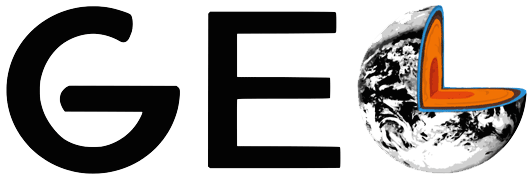
\includegraphics[height=1cm]{figures/logos/geg.png}
\end{center}}
%\makeatother

\begin{document}
\title{Annual report 2019:\\
\emph{Reaktoro as the chemical reaction solver in Shell's reservoir simulator}}
\author{Allan M. M. Leal and Svetlana Kyas \\
{\scriptsize Institute of Geophysics, Department of Earth Sciences, ETH Z\"urich, Switzerland}}
\date{02.12.2019}

\maketitle

%---------------------------------------------------------------------------------------------------%
\begin{abstract}
The report summarizes the results obtained during the first year of the project ``Reaktoro as 
the chemical reaction solver in Shell's reservoir simulator'. It is mainly focused on the first task 
of the project plan, i.e., ``Accelerating chemical kinetics in reactivate transport calculations''. 
\end{abstract}

\begin{comment}
\sveta{Below, we provide the motivation of the this task. During the reactivate transport modeling, 
the computational cost associated with chemical equilibrium and chemical kinetics speciation 
calculations can be 10–10'000 times higher than that of fluid flow and solute transport simulations. 
Such geochemical calculations must be performed in each mesh cell at every time step of the simulation, 
incurring high computing costs. To radically reduce these, we consider a new \emph{on-demand machine 
learning strategy} (ODML) (also referred as \emph{smart algorithm}) that, during reactive transport 
simulations, enables the chemical speciation to be quickly and accurately predicted using stored 
results of previously evaluated chemical equilibrium or kinetics calculations performed within 
the simulation session. 
%
We demonstrate the applicability and utility of this algorithm in a reactive transport modeling 
example, where it yields a calculation speedup of one-two orders of magnitude. The implementation 
and numerical tests are carried out in Reaktoro, a unified, open-source framework for modeling 
chemically reactive systems. Further research plans and ideas to improve considered algorithm are 
also summarized.}
\end{comment}

\section*{Report Summary}

This section provides a short summary of the results achieved this year as well as the outlook of 
main future tasks and steps of further investigation. 

{\bf Results}
%---------------------------------------------------------------------------------------------------%
\begin{enumerate}\setlength{\itemsep}{0pt} \setlength{\parskip}{0pt}
\item The on-demand learning machine algorithm (ODML) was tested on the one-dimensional reactive 
transport problem, where chemistry is controlled by local equilibrium and Pitzer activity model for 
the aqueous species. After extensive tests of such chemical system with 36~species in 4~phases, 
the following results have been obtained:
%
%---------------------------------------------------------------------------------------------------%
\begin{itemize}
\setlength{\itemsep}{0pt} \setlength{\parskip}{0pt}
\item Application of the ODML algorithm yields speedup of {\bf 200} (in the worst case) and 
{\bf 400} (in the best / zero-cost-search case) for chemical calculation in reactive transport 
simulations.
%
\item Only {\bf 258} chemical states out of {\bf 1,000,000} has been evaluated fully (by triggering 
Gibbs energy minimization (GEM) problem), the rest {\bf 99.97} \% of the cells are estimated in 
a quick and accurate way.
%
\item The relative error of the approximations provided by the smart approach (in comparison to 
the conventional approach) is less than 1\% in mineral's phase-volumes and less than 4\% 
in the aqueous species.  
%
\item Main results, obtained by testing the algorithm on the above-described benchmark, are 
summarized in the report \cite{Leal2017d} and submitted to the Journal of Transport in Porous Media 
(TIPM).
\end{itemize}
%
\item The ODML algorithm was extended the reactive transport problem with chemical kinetics. 
Extended tests on the one-dimensional benchmark example with Calcite assumed to be controlled 
kinetically has provided the following results:
%
\begin{itemize} 
\setlength{\itemsep}{0pt} \setlength{\parskip}{0pt}
\item Application of the smart chemical kinetics algorithm alone provides a speedup of {\bf 8-10x}
%
\item Application of the smart chemical kinetics algorithm together with smart equilibrium provides 
speedup of {\bf 30x} and {\bf 100x} (in the worst and best case, respectively).
%
\end{itemize}
%---------------------------------------------------------------------------------------------------%
%
\item Application of the ODML method to the systems with more than one kinetically controlled 
reactions indicates a potential for even higher speedups, i.e., {\bf 35-102x} for two and 
{\bf 92-124x} for tree kinetic species.
%
\item \texttt{Reaktoro} has been coupled with open-source partial differential equations (PDEs) 
solver \texttt{Firedrake} for modeling high-dimensional heterogeneous reactive transport problems 
as well as further testing and improvement of the ODML algorithm on more challenging scenarios.   
\end{enumerate} 

%---------------------------------------------------------------------------------------------------%
{\bf Future tasks}
%
\begin{enumerate} \setlength{\itemsep}{0pt} \setlength{\parskip}{0pt}
\item Improvement of the acceptance criterion in the ODML algorithm (providing fewer learnings 
together with high accuracy).
%
\item Improvement of the time for the reference element retrieval/search/lookup with 
%---------------------------------------------------------------------------------------------------%
\begin{itemize} 
\setlength{\itemsep}{0pt} \setlength{\parskip}{0pt}
\item combination of tree-based (kd-tree) and linear search algorithms,
\item locally sensitive hashing tables (LSH),
\item using reference points clustering/ranking.
\end{itemize}
%---------------------------------------------------------------------------------------------------%
%
\item Including smart chemical equilibrium algorithm into the right-hand (RHS) evaluation of 
the system of ODEs governing kinetically controlled species, which can cause up to hundreds of 
chemical equilibrium calculations.
%
\item Extension of the smart approach to the evaluation of the chemical properties that might 
improve performance of the reactive transport simulations, generally.
%
\item Testing the ODML algorithm on more complex benchmarks:
%---------------------------------------------------------------------------------------------------%
\begin{itemize} 
\setlength{\itemsep}{0pt} \setlength{\parskip}{0pt}
\item more advanced chemical systems, such as reactive transport for the rich chemical system, where 
cement is attacked by seawater or NaCl brine (represented by 170 species with about a dozen of 
different phases, including complex multi-mineral phases),
\item chemical systems with more then one kinetically controlled species,
\item reactive transport in two- and three-dimensional heterogeneous porous media.
\end{itemize}
%---------------------------------------------------------------------------------------------------%
%
\end{enumerate}

\section{Introduction}

%---------------------------------------------------------------------------------------------------%
In reactive transport simulations, coupled chemical and physical processes are modeled to understand 
phenomena that involve the transport of chemical species (i.e. reactants) and chemical reactions. 
Examples of chemical processes are reactions between species in an aqueous fluid leading to 
precipitation of solid minerals, or their reaction with existing rock minerals causing mineral 
dissolution (see \cite{Lichtner1985, Steefel2005, Steefel2019} and references therein). Examples of 
physical processes are the advection of chemical species in a fluid that flows with a certain 
velocity, or the diffusion of those fluid species as a result of the concentration gradient across 
the medium. Because of the various processes combined into a reactive transport model, the resulting 
computer simulations are usually time-consuming.

%---------------------------------------------------------------------------------------------------%
Often, the relatively long computing time of reactive transport simulations can be largely attributed 
to the need of performing millions to billions of chemical reaction calculations, in particular, 
\emph{chemical kinetics} and\slash or \emph{equilibrium speciation calculations} performed in every 
mesh cell during every time step of the simulation. These chemical reaction calculations are 
computationally expensive because they involve iterative algorithms to solve systems of non-linear 
algebraic and\slash or system of ordinary differential equations (ODEs) \citep{Leal2017}. As a result, 
they trigger repeated evaluations of thermodynamic properties, such as activity\slash fugacity 
coefficients (sometimes using computationally demanding models such as \citet{Pitzer1973} for aqueous 
phases and \citet{Peng1976} for gaseous/liquid phases).

%---------------------------------------------------------------------------------------------------%
Thus, speeding up reactive transport modeling by a significant factor may only be accomplished by 
first accelerating chemical reaction calculations in general. Advancing chemical equilibrium speciation 
calculations is essential when employing a \emph{partial local chemical equilibrium assumption} 
\citep{Ramshaw1980,Ramshaw1981,Ramshaw1985,Ramshaw1995,Lichtner1985,Steefel1994,Steefel1996}.
This assumes that the species that are reacting at relatively high rates (typically aqueous or gaseous 
species) are in a state of continual chemical equilibrium in each mesh cell. In contrast, the species 
reacting at slow to moderate rates (typically minerals) do so according to kinetic rate laws and, 
hence, are not in equilibrium with the rest of the system. Thus, accelerating those millions to 
billions of chemical calculations over the course of a massive numerical reactive transport simulation 
is essential when using fine-resolution meshes, large three-dimensional domains, and\slash or long 
simulation times at fine temporal resolution.

%---------------------------------------------------------------------------------------------------%
Major advances in developing fast, accurate, and robust methods for chemical equilibrium calculations, 
in particular, have been achieved over the past decades. These are either based on 
\emph{Gibbs energy minimization} (GEM) or \emph{law of mass action} (LMA) formulations 
\citep{White1958,Smith1980,Smith1982,Alberty1992b,Crerar1975,DeCapitani1987,Eriksson1989,Ghiorso1994,
Gordon1971,Gordon1994a,Gordon1996,Harvey2013,Harvie1987,Karpov1997,Karpov2001,Karpov2002,Koukkari2011a,
Kulik2013,Leal2013,Leal2014,Leal2016a,Leal2016c,Leal2017,Morel1972,Neron2012,Nordstrom1979,
Trangenstein1986,VanZeggeren1970,Vonka1995,Wolery1975,Zeleznik1960}.
%
However, even if one could devise a hypothetical algorithm that would always converge in a single 
iteration, instead of the typical few to dozens of iterations, the computational cost of chemical 
equilibrium calculations could still be dominant in a reactive transport simulation. This is the case, 
as during this single iteration expensive thermodynamic models would still have to be evaluated and 
matrix equations have to be solved (using a Newton-based GEM or LMA algorithm). In view of this, 
a substantial acceleration of these calculations can be achieved if those costly operations
can be bypassed whenever possible. 
\sveta{
Similarly, advanced methods for solving a system of differential equations has been 
developed during a couple of last decades \cite{Ascher1998,HairerNorsettWanner1993,HairerWanner1996}. 
Due to rapid variations in some of the species' reaction rates, the behaviour of kinetically-controlled 
species are often represented by the stiff system of ODEs, which adds additional difficulty. 
However, we aim to apply such an approach that sidesteps costly numerical integration of the system 
that governs the evolution of kinetics species within considered transport step.
}
\begin{figure}[!t]
	\centering
	\subfloat[]{
	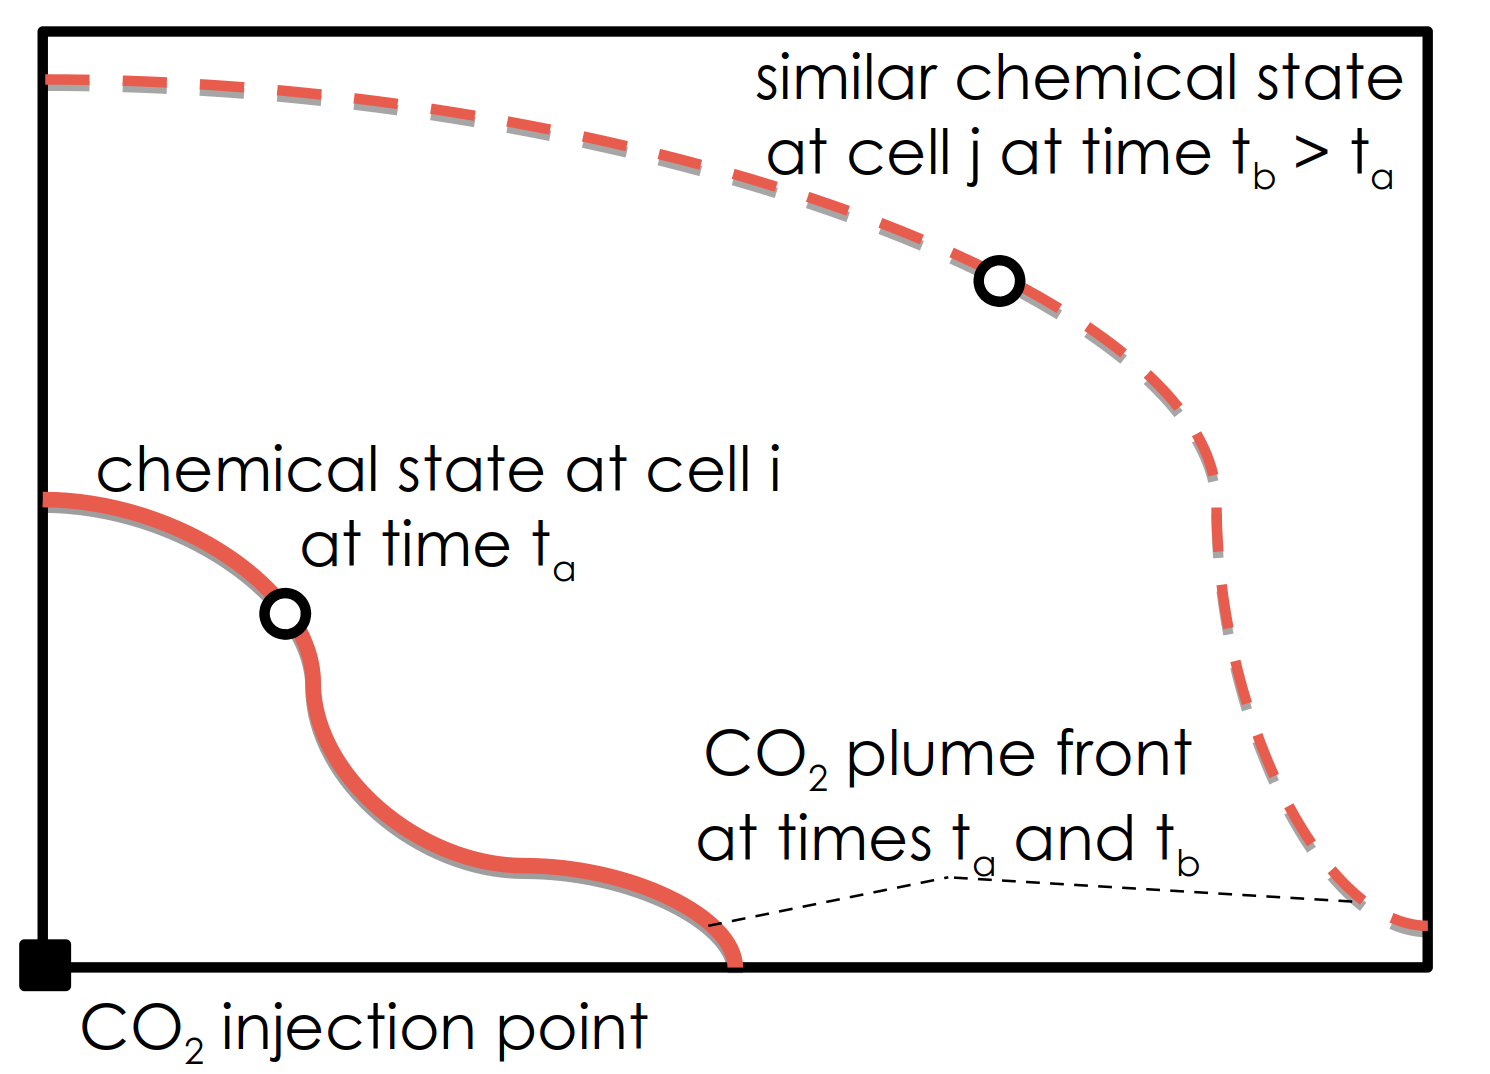
\includegraphics[height=6cm]{figures/intro/similar-equilibirum}
	\label{fig:similar-equilibrium}}
	\quad
	\subfloat[]{
	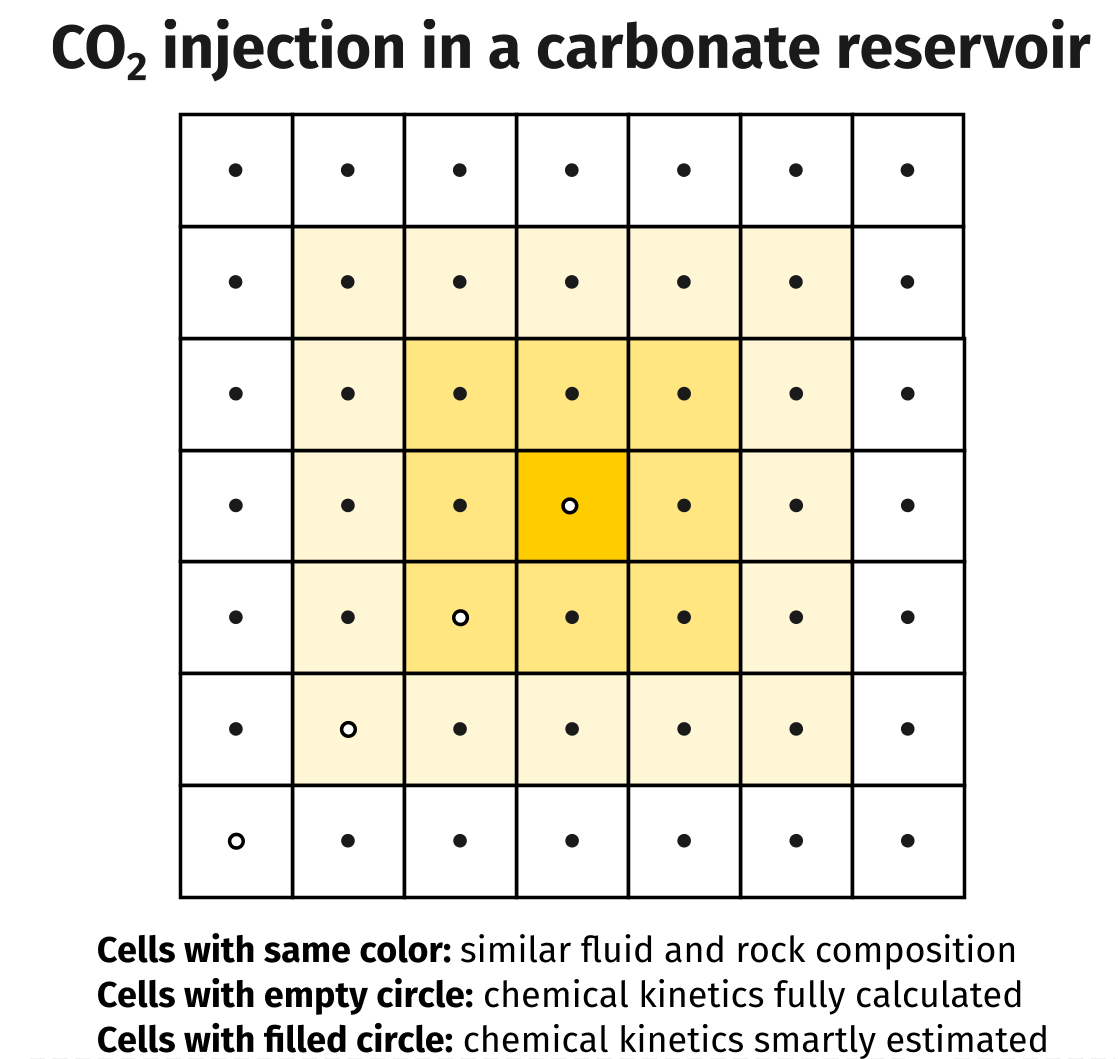
\includegraphics[height=6cm]{figures/intro/similar-kinetics}
	\label{fig:similar-kinetics}}
	\caption{Example of similar chemical speciations encountered in chemical equilibrium and kinetics.}
	\label{fig:similar-equilibrium-kinetics}
\end{figure}

%---------------------------------------------------------------------------------------------------%
During a single time step of a reactive transport simulation, chemical kinetics and equilibrium
calculations are needed in all mesh cells. Often, many of these calculations are similar to previously 
performed ones, either within the same time-step and\slash or mesh cell or at different points in 
space and\slash or time (see Figure \ref{fig:similar-equilibrium-kinetics}). We assume two chemical 
equilibrium problems to be similar when their input conditions are sufficiently close (i.e., similar 
temperature, pressure, amounts of chemical elements, and the electric charge of each phase, containing 
electrically charged species \citep{Smith1982}). At the same time, these chemical equilibrium 
calculations are hardly identical so that we cannot simply assume a previously computed chemical 
speciation as the exact result of the new calculation. Interpolating is also not an appropriate
approach, as it can violate the \emph{mass conservation} of elements (i.e., there is a deviation 
between the input element amounts and the amounts of elements calculated from the interpolated species 
amounts). 

%---------------------------------------------------------------------------------------------------%
The main principle of the \emph{ODML algorithm} suggested here is precisely to \emph{avoid} as much as 
possible full and expensive chemical speciation calculations during the reactive transport simulation. 
That is why it is often referred to as \emph{smart chemical equilibrium algorithm}. By using 
\emph{sensitivity derivatives} of previously computed chemical equilibrium states, we can quickly 
and accurately estimate the new equilibrium state (chemical speciation) under similar input conditions
(see Figure \ref{fig:similar-equilibrium}). These derivatives provide an insight into how sensitive
the computed species amounts at a certain equilibrium state are with respect to infinitesimally small 
changes in temperature, pressure, and amounts of chemical elements. Thus, multiplying these sensitivity 
derivatives by the respective differences in input conditions (e.g., differences in temperature
or the amount of a particular element), we can predict the variation in the output. For example, we 
can estimate how much the species amounts would change by increasing temperature by 1~°C, by adding 
1~mmol of HCl into the system (which is equivalent to adding 1~mmol of elements H and Cl), or by 
combining these with other input changes. We remark that the use of sensitivity derivatives to estimate 
the solution of an equilibrium problem is inherently \emph{mass conservative}, since they are being 
computed along with he derivation of chemical equilibrium equations (with equations of element mass 
conservation included).

%---------------------------------------------------------------------------------------------------%
\sveta{
For kinetically controlled species, one can find similarities in their initial 
states at each transport step. Figure \ref{fig:similar-kinetics} illustrates possible perturbations 
of fluid/rock compositions in mesh cells discretising two-dimensional reservoir. \emph{Smart chemical 
kinetics algorithm} will perform numerical integration of the system of kinetic species only for 
some uniquely distinguishable initial states (marked with empty circles in Figure 
\ref{fig:similar-kinetics}). Simultaneously, we also recover additional information about their 
sensitivities with respect to infinitesimal changes in the initial condition. In the rest of the 
subsequently encountered cells, we attempt to make \emph{smart prediction} of the possible kinetic 
speciation at the end of the transport step, exploiting information collected in the previous 
mesh-cells.
}

\subsubsection*{Related Work}

Increasing the speed of chemical speciation calculations, whether it is equilibrium and\slash or 
kinetics, is an active research topic. The majority of the existing methodologies are based on the use 
of \emph{surrogate models} and\slash or \emph{statistically based machine learning} schemes, which use 
a computationally cheaper model (e.g., linearization, parameterization, convolutional neural network) 
to approximate a complex nonlinear behavior.

%---------------------------------------------------------------------------------------------------%
In combustion chemistry, the pioneering work of \citet{Pope1997} in accelerating \emph{chemical 
kinetics calculations} considered approximations of chemical kinetics paths using multiple linear 
regressions, employing \emph{unstructured adaptive} \emph{storage/extraction techniques} along 
the simulation process. This approach is referred to in the literature as the \emph{in-situ adaptive 
tabulation} (ISAT) algorithm. The ISAT approximation idea was later extended to \emph{nonlinear
model predictive control} (NMPC) in \citep{HedengrenEdgar2008}. ISAT can be regarded as an alternative 
to artificial neural networks, as it does not require any preliminary training to simulate the 
behavior of the model. Instead, it rearranges the model by the training on new data \emph{on the 
fly}, as simulations proceed. The ISAT algorithm scales quadratically with increased dimension, 
approximates functions with discontinuities, and provides explicit bounds on approximation errors. 
Recent improvements of the ISAT algorithm and\slash or its demonstration for the simulation of 
unsteady, compressible, reactive flows can be found in 
\cite{Singer2004,Singer2006,Lu2007,Pope2009,Lu2009}.
%
A series of parallel chemistry acceleration algorithms using different distribution strategies for
simulation of unsteady, compressible, reactive flows, based on the ISAT technique, was implemented in 
the software \texttt{\href{https://tcg.mae.cornell.edu/x2f\_mpi/}{${\rm x2f_mpi}$}} \cite{x2fmpi2006} 
and studied for the numerical simulations of a two-dimensional gaseous detonation wave propagation 
process in \citet{Dong2007,Dong2009,WuDongLi2018}. 

%---------------------------------------------------------------------------------------------------%
In addition to the ISAT approach, several alternative storage-based approaches have been suggested in 
the past for accelerating chemical kinetics calculations, including polynomial fits \citet{Turanyi1994}, 
artificial neural networks (see, e.g., \citet{ChristoMasriNebot1996,Blascoetall1998}), and piece-wise 
reusable implementation of solution mapping (PRISM) by \citet{TonseMoriartyBrownFrenklach2013}. The 
common property of these approaches is the a priori creation of the approximation model (whether it 
is a skeleton model or a neural network), which usually requires extra effort to then evaluate a 
simplified model that accelerates subsequent calculations. The PRISM method is similar to the in-situ 
approach, except that the stored data entries are not output values and corresponding sensitivity 
derivatives, but rather the set of polynomials, covering a region of chemical composition space. 
The observed acceleration for these methods is about a factor of 10-60.

%---------------------------------------------------------------------------------------------------%
The work of \citet{Jatnieks2016}, on the use of a surrogate model for fast speciation calculations, 
is another initiative to accelerate chemical equilibrium calculations during reactive transport 
modeling. The construction of this surrogate model required a training stage in advance of the 
simulation of interest, during which many random input conditions are used in PHREEQC 
\citep{Parkhurst2013}, and the resultant outputs collected for statistics-based 
learning. During their numerical experiment,~32~different statistical and machine learning methods
were tried to identify the potentially best one. For a specific reactive transport modeling problem, 
\citet{Jatnieks2016} collected all possible input-output combinations in speciation calculations, and 
from these, 7880 input-output samples, representing 80\% of the total known input-output relationships, 
were used for training the statistical model. The various constructed surrogate models were subsequently 
used in the reactive transport simulation. Because these surrogate models relied on statistical methods, 
mass conservation was often not accurate during their machine learning computations (i.e., the amounts 
of chemical elements in the estimated-output species amounts did not correspond accurately to the 
values given in the input). 

The work \cite{Laloy2019} presents a comparison of several approaches 
(Gaussian processes (GP), polynomial chaos expansion (PCE) and deep neural networks (DNNs)), which are 
used to emulate CPU-intensive reactive transport models. However, considered methods are subjected 
to uncertainties propagation and, as the result, deteriorating accuracy. For relatively simple problems 
DNNs performed the best (even having relatively small training sets), providing the most accurate 
representation of results. However, the DNN approach leads to the worst solution of the considered 
synthetic inverse problem due to the small but rather complicated deterministic noise that affects 
the DNN-based predictions. Also, for more complicated problems DNN produces quite disperse outputs, 
which only confirms the difficulty of finding emulator able to replace the entire reactive transport 
process with all its complex behaviours and possible outcomes. The approach proposed in our work 
focuses only on speeding up the chemical part of the entire simulation, which narrows down the number 
of physical effects influencing the input space and, as results, allows finding more similarities 
triggering more smart predictions.
%
Moreover, unlike the ``black-box'' representation of the complex original model used by methods in 
\cite{Laloy2019}, our approach ``remembers'' the most crucial properties of the chemical system under 
consideration (such as mass balance equation, sensitivity derivatives, ect.), allowing to maintain 
the requested accuracy of simulations' results.

%---------------------------------------------------------------------------------------------------%
The \emph{on-demand learning approach} developed here exhibits several advantages over conventional 
statistics- or neural network-based machine learning methods. Firstly, the use of \emph{sensitivity 
derivatives} of the calculated equilibrium states results in a method that better reflects the behavior 
of chemical systems and how they react to subsequent changes in input equilibrium conditions. Secondly, 
the use of these sensitivity derivatives permits predicting new equilibrium states \emph{without a 
loss of accuracy and confidence}. Thirdly, the proposed method requires \emph{no a priori statistical 
training} before it can be applied in a reactive transport simulation. Its on-demand machine learning 
characteristics enable spontaneous learning of only what is needed to be calculated anew during 
a reactive transport simulation to keep new predictions accurate enough. Note that, when using 
a conventional chemical equilibrium calculation approach, these computations are needed anyway. 

%---------------------------------------------------------------------------------------------------%
Furthermore, discussed here on-demand learning strategy is not only simpler from an end-user point 
of view (as no a priori training stage needs to be performed), but also likely faster. It will, 
in general, require saving far fewer input conditions and computed chemical speciations than any 
statistical approach, which can only get the more accurate the more it trains in advance, and where 
the amount of useful training calculations is unknown. This lack of knowledge typically leads to 
the calculation of many more chemical reaction results than what may ever be needed during the actual 
simulation, with a risk that actually required calculations may not have been part of the a priori 
training set at all. This is akin to going to school to learn all sorts of things, most of which are 
never needed later on for a specific job at hand. 

%---------------------------------------------------------------------------------------------------%
Finally, the smart chemical equilibrium algorithm produces output speciations that \emph{always 
satisfy conservation conditions} for chemical elements and electric charge, as these constraints are 
incorporated into the calculation of the sensitivity derivatives (see \citet{Leal2017}). This, in 
particular, distinguishes the discussed method from the statistics-based machine learning methods, 
which can lose precision or fail in this respect.

Some similarities may inevitably exist between the \emph{on-demand machine learning} (ODML)
algorithm and other existing strategies for speeding up chemical equilibrium 
and\slash or chemical kinetics calculations. Existing techniques, for example, that 
rely on interpolation, may also require search operations and decision making whether 
to accept or not the interpolated estimate. However, the major current (and also future) 
differences are that ODML
%
\begin{enumerate}[wide, labelwidth=!, labelindent=0pt]
\item[\emph{(i)}] aims to be a more \textbf{general-purpose acceleration algorithm} that could also 
be applied for other types of expensive and repeated computations (e.g. evaluations of fluid 
thermo-physical properties) instead of being applied exclusively to chemical equilibrium \slash or 
chemical kinetics problems;
%
\item[\emph{(ii)}] can use \textbf{higher-order sensitivity derivatives} for improved predictive 
accuracy that reduces the number of on-demand training operations, and provide superior error 
analysis (detailed in a future communication);
%
\item[\emph{(iii)}] provides the capability for \textbf{more flexible error controls} that may 
consider chemical, physical, and\slash or engineering insights on the acceptance decision, instead 
of relying on statistics or geometric considerations (e.g., using hyper-ellipsoids confidence regions); 
and, finally,
%
\item[\emph{(iv)}] uses \textbf{alternative search operations} that do not rely exclusively on 
the nearest neighbor search, which is prone to fail for high-dimensional input spaces (commonly-known 
in the statistical and machine learning literature as the \emph{curse of dimensionality}).
\end{enumerate}
%
%---------------------------------------------------------------------------------------------------%
A dedicated C++ library project for ODML is envisioned, in which the exact higher-order sensitivity
derivatives mentioned previously are calculated using 
\texttt{\href{http://autodiff.github.io}{autodiff}} (\citealt{autodiff}), a modern and fast C++ 
library for higher-order automatic differentiation computations, whose on-going development is 
specifically carried out towards achieving the planned algorithm's goals.

%---------------------------------------------------------------------------------------------------%
\subsubsection*{Organization}

This report is organized as follows:
\begin{enumerate}[wide, labelwidth=!, labelindent=0pt]
\item [{\bf Section~\ref{sec:Definitions-and-Notation}}] introduces definitions and the notation 
needed to describe the algorithm.
\item [{\bf Section~\ref{sec:Method}}] formulates the smart chemical equilibrium and kinetics 
algorithms with details regarding the learning and prediction operations.
\item [{\bf Section~\ref{sec:Results}}] demonstrates the performance and accuracy of a reactive 
transport simulation, using the smart chemical equilibrium and kinetics algorithms. 
%
\sveta{
It consists of three parts 
with results corresponding to three major stages of development of smart algorithm. The first tests
of the algorithm were focused on studying its performance in the reactive transport model with all 
the species controlled
by equilibrium and with Pitzer activity model used (see Subsection \ref{subsec:part-1}). 
%
Subsection \ref{subsec:part-2} is dedicated to describing the performance of the smart approach on 
the chemical system with kinetically controlled species. 
%
Finally, Subsection \ref{subsec:part-3} highlights results of reactive transport simulations 
obtained after coupling \texttt{Reaktoro} with \texttt{Firedrake}, an automated system for the 
solution of partial differential equations using the finite element method (FEM) \cite{Rathgeber2016}.
}
\item [{\bf Section~\ref{sec:Discussion-and-Conclusions}}] discusses implications and conclusions of 
this report together with a detailed road-map for further research efforts in this direction.
\end{enumerate}


%---------------------------------------------------------------------------------------------------%
\section{Definitions and Notation\label{sec:Definitions-and-Notation}}

Considered throughout the paper, a \emph{chemical system} is a collection of \emph{chemical species} 
composed of one or more \emph{elements} and distributed among one or more \emph{phases}. The species 
can be substances such as aqueous ions (e.g., Na$^{+}$(aq), Cl$^{-}$(aq), HCO$_{3}^{-}$(aq)), neutral 
aqueous species (e.g., SiO2(aq), CO$_{2}$(aq), H$_{2}$O(l)), gases (e.g., CO$_{2}$(g), CH$_{4}$(g), 
N$_{2}$(g)), pure condensed phases (e.g., CaCO$_{3}$(s, calcite), SiO$_{2}$(s, quartz), 
Al$_{2}$Si$_{2}$O$_{5}$(OH)$_{4}$(s, kaolinite)), etc. Each phase (e.g., aqueous, gaseous, liquid, 
solid solutions, a pure mineral, plasma, etc.), having homogeneous properties within its boundaries 
is composed of one or more different chemical species (components, end members). Multi-component 
phases are also called \emph{solutions}, where components are mixed within the same structure.  
The elements (independent components) are \emph{chemical elements} (e.g., H, O, C, Na, Cl, Ca, Si) 
and \emph{electrical charge} (Z), but can also be linear combinations of these, commonly known as 
\emph{primary species} (e.g., H$^{+}$(aq), H$_{2}$O(l), CO$_{2}$(aq)).

A chemical system can exist at infinitely many \emph{chemical states}. A chemical state is defined 
here as the quadruplet $(T, P, n, b)$, where $T$ is temperature, $P$ is pressure,  
$n=(n_{1},\ldots,n_{\mathrm{N}})\in\mathbb{R}^{{\rm N}}$ is the vector of species amounts 
(speciation), with $n_{i}$ denoting the amount of the $i$th species (in moles) and N the number of 
species, and $b=(b_{1},\ldots,b_{\mathrm{E}})\in\mathbb{R}^{{\rm E}}$ is the vector of element 
amounts with $b_{j}$ being the amount of the $j$th element (in moles) and ${\rm E}$ the number of 
elements. In general, $b$ is related to $n$ via the following mass conservation equation:
%
\begin{equation}
An=b,
\label{eq:mass-balance}
\end{equation}
%
where $A$ is the \emph{formula matrix} of the chemical system \citep{Smith1982} (whose dimensions 
are $\mathrm{E}\times\mathrm{N}$), with $A_{ji}$ denoting the coefficient of the $j$th element in 
the $i$th species.

\sveta{
In order to consider a system with kinetically controlled species, we assume the partition of the 
speciation to equilibrium and kinetic species with corresponding amounts 
$n_{e} \in \mathbb{R}^{{\rm N}_e}$ and $n_{k} \in \mathbb{R}^{{\rm N}_k}$, where 
${\rm N} = {\rm N}_e \cup {\rm N}_k$, and corresponding elements compositions 
$b_{e}, b_{k} \in \mathbb{R}^{\rm E}$. Then, the total amount of chemical species is presented as 
\[
n=\begin{bmatrix}n_{e}\\n_{k}\end{bmatrix} \in \mathbb{R}^{\rm N}
\]
with the formula matrix $A=\begin{bmatrix}A_{e}\;A_{k}\end{bmatrix}$ composed of 
matrices of the equilibrium and kinetic species $A_{e}$ and $A_{k}$, respectively. 
}
%---------------------------------------------------------------------------------------------------%
\section{Method\label{sec:Method}}

Let the dependence of $n_{e}$ from $b_{e}$ be prescribed by the abstract chemical equilibrium function 
%
\begin{equation}
n_{e}=\varphi(b_{e}),\varphi:\mathbb{R}^{E}\rightarrow\mathbb{R}^{N},
\label{eq:equilibrium-func}
\end{equation}
%
that encapsulates the specific algorithmic steps to solve the fundamental Gibbs energy minimization 
problem
%
\[
\varphi(b_{e}):={\rm argmin}_{n_{e}} G_{e} = n_{e}^{T} \mu_{e}
\quad\mbox{s.t.}\quad
\begin{cases}
A_{e} \, n_{e} & =b_{e}\\
n_{e} & \geq0
\end{cases}.
\label{eq:gem-problem}
\]
%
The \emph{chemical potential} of the $i$th species $\mu_{e, i}=\mu_{e, i}(T,P,n_e)$ is defined as:
%
\begin{equation}
\mu_{e, i}=\mu_{e, i}^{\circ}+RT\ln a_{e, i},
\end{equation}
%
with $R$ denoting the universal gas constant, $\mu_{e, i}^{\circ}=\mu_{e, i}^{\circ}(T,P)$ the 
\emph{standard chemical potential} of the $i$th species, and $a_{e, i}=a_{e, i}(T,P,n_e)$ the 
\emph{activity} of the $i$th species. Methods for solving chemical equilibrium problem using either 
Gibbs energy minimization (GEM) or the law of mass action (LMA) methods are addressed in 
Appendix~\ref{subsec:Chemical-equilibrium-equations} or with more detail in 
\citet{Leal2016a,Leal2016c,Leal2017} and references therein.

\sveta{
%---------------------------------------------------------------------------------------------------%
The amounts of the kinetic species $n_{k}$ are governed by the system of ordinary differential 
equations (ODEs)
%
\begin{equation}
\begin{array}{r@{$\;$}l@{$\quad$}l}
	\frac{dn_{k}}{dt} & = r(n_{k}) + q_{k} & t>0,\\
                n_{k} & = n_{k}^{\circ}    & t=0,
\end{array}
\label{eq:kinetics}
\end{equation}
%
%---------------------------------------------------------------------------------------------------%
where $r$ are the \emph{rates} of the kinetically controlled reactions,  $q_{k}$ denotes 
the \emph{vector of inflow/outflow} rates of the kinetic species, and $n_{k}^{\circ}$ is
the \emph{initial amounts} of the kinetic species. 

{\bf Note}: To make the explanation more transparent, in Eq.~\eqref{eq:kinetics} we consider a 
simplified version of the system of ODEs that govern kinetically controlled species. For a more 
detailed derivation of the differential-algebraic system to describe the \emph{chemical state of a 
system}, we refer to Appendix~\ref{subsec:Chemical-kinetics-equations} or previous works 
\citet{Leal2015,Leal2017} and references therein.
}

\subsection{First-Order Taylor Approximation\label{subsec:First-order-Taylor-approximation}}

%---------------------------------------------------------------------------------------------------%
Assume that a chemical equilibrium calculation has been performed previously with input conditions
$(T^{\star},P^{\star},b^{\star}) = (T,P,b)^\star$, and a new one needs to be performed with 
$(T,P,b)$ instead. 
%
Rather than computing $n_e=\varphi(T,P,b_e)$, using the computationally expensive equilibrium 
function $\varphi$ (cf. \ref{eq:equilibrium-func}), we first try estimating $\bar{n}_e$ with a 
\emph{first-order Taylor approximation}:
%
\begin{equation}
\bar{n} = 
n^{\star}+\frac{\partial\varphi}{\partial T}^{\star}(T-T^{\star})
+\frac{\partial\varphi}{\partial P}^{\star}(P-P^{\star})
+\frac{\partial\varphi}{\partial b}^{\star}(b-b^{\star}),
\label{eq:smart-estimate}
\end{equation}
%
where $(\partial\varphi/\partial T)^{\star}$, $(\partial\varphi/\partial P)^{\star}$, and 
$(\partial\varphi/\partial b)^{\star}$ are \emph{sensitivity derivatives} of the reference chemical 
equilibrium state, which can be equivalently written as $(\partial n/\partial T)^{\star}$, 
$(\partial n/\partial P)^{\star}$, and $(\partial n/\partial b)^{\star}$, respectively. If computed 
together with the full speciation vector $n$, these sensitivity derivatives will allow us to estimate 
how the species amounts in an equilibrium state change when small perturbations are applied to 
temperature, pressure, and\slash or amounts of elements, and, therefore, quickly and accurately 
estimate entirely new states in the vicinity of some previous and fully calculated chemical 
equilibrium state.

\sveta{
%---------------------------------------------------------------------------------------------------%
In case of kinetically controlled species, the similar approach can be applied. We use 
the sensitivities of species $n_k$ with respect to the small perturbation in the initial condition 
$n_k^\circ$ defined as
%
\[
\frac{\partial n_k}{\partial n_k^\circ}. 
\label{eq:sensitivities}
\]
%
%---------------------------------------------------------------------------------------------------%
Let $\Big(\tfrac{\partial n_k}{\partial n_k^\circ}\Big)^\star$ be stored along with $n^\star_k$ 
(result of numerical integration of the system defined by Eq.~\eqref{eq:kinetics}) and the initial 
state $\big(n^\circ_k\big)^\star$. Then, instead of evaluating new chemical state with the initial 
condition $n^\circ_k$, the kinetic species can be approximated as follows:
%
\begin{equation}
\bar{n}_k 
= n^\star_k + \delta n_k
= n^\star_k + \Big(\frac{\partial n_k}{\partial n_k^\circ} \Big)^\star \, 
\big(n^\circ_k - (n^\circ_k)^\star \big)
\label{eq:smart-estimate-kinetics}
\end{equation}
%
If $\bar{n}_k$ is accurate enough, the computationally costly numerical integration of the system 
\eqref{eq:kinetics} is replaced by matrix-vector multiplication formula 
\eqref{eq:smart-estimate-kinetics}. 
}

\begin{comment}
% more detailed explanation

%---------------------------------------------------------------------------------------------------%
In case, of kinetically controlled species similar logic can be applied. We introduce the property 
that measures how sensitive species $n_k$ w.r.t. the choice of initial condition $n_k^\circ$. It is
called \emph{sensitivity} and defined as
%
\[
s(t) := \frac{\partial n_k}{\partial n_k^\circ}(t). 
\]
%
%---------------------------------------------------------------------------------------------------%
Let $s^\star = \Big(\tfrac{\partial n_k}{\partial n_k^\circ}\Big)^\star$ be evaluated and stored 
along with $n^\star_k$ after numerical integration has been performed with initial state 
$\big(n^\circ_k\big)^\star$. Then, provided with a new initial condition for the kinetic species 
$n^\circ_k$, $\bar{n}_k$ can be approximated as follow:
%
\begin{equation}
\bar{n}_k 
= n^\star_k + \delta n_k
= n^\star_k + s^\star \, \delta n^\circ_k 
= n^\star_k + \Big(\tfrac{\partial n_k}{\partial n_k^\circ} \Big)^\star \, 
\big(n^\circ_k - (n^\circ_k)^\star \big)
\label{eq:smart-estimate-kinetics}
\end{equation}
%
Analogously to Eq. \ref{eq:smart-estimate}, the complex numerical integration of the system 
\eqref{eq:kinetics} is replaced by matrix-vector multiplication formula 
\eqref{eq:smart-estimate-kinetics}. Here, sensitivity is a matrix $s\in\mathbb{R}^{N\times N}$ that 
satisfies the following system of ODEs
% 
\begin{align*}
\frac{d s}{dt} & = J_r (n) \, s & t>0,\\
             s & = I            & t=0,
\end{align*}
%
where ${J}_{r}$ is a Jacobian of $r(n_k)$, and ${I} \in \mathbb{R}^{N \times N}$ is the identity 
matrix.
\end{comment}

%---------------------------------------------------------------------------------------------------%
\subsection{Nearest Neighbor Search\label{subsec:Nearest-Neighbor-Search}}

Let 
%
\begin{equation}
\mathcal{I}_e =\left\{ (T,P,b_e)^{\,i}\right\}_{i=1}^{{\rm I}} 
\qquad \mbox{and} \qquad 
\mathcal{I}_k =\left\{ (n^{\circ}_k)^{\,j} \right\}_{j=1}^{{\rm J}}
\end{equation}
%
represent the sets of input conditions for the chemical equilibrium and kinetics problems, 
respectively, that have been fully solved (i.e., using the chemical equilibrium function $\varphi$ 
or system of ODEs \eqref{eq:kinetics}).
%
\sveta{
%---------------------------------------------------------------------------------------------------%
Furthermore, let 
%
\begin{equation}
d^{i}_e = \left[
\left(T-T^{i}\right)^{2} 
+\left(P-P^{i}\right)^{2}
+\sum_{l=1}^{{\rm E}}\left(b_{l}-b_{l}^{i}\right)^{2}\right]^{\frac{1}{2}} 
\qquad \mbox{and} \qquad 
d^{j}_k = \left[ \sum_{m=1}^{{\rm N_k}} 
n^\circ_{k, m} - \left((n^\circ_{k, m})^{\,j}\right)^2 \right]^{\frac{1}{2}} 
\end{equation}
%
denote the Euclidean distances either from $(T, P, b_e)^i$ to $(T,P,b)$ or from 
$(n^\circ_{k})^{\,j}$ to $n^\circ_{k}$. In $d^{i}_e$, the input condition of the $i$th fully 
solved problem and the given input condition for the new equilibrium calculation are compared, 
whereas $d^{j}_k$ measures the distance between the initial condition of $j$th fully integrated 
problem and the initial condition of new one.
}

%---------------------------------------------------------------------------------------------------%
\textbf{Note:} Other norms can be used to define the distance measure above and other search 
operations can be equally considered (not necessarily based on the nearest neighbor, which can be 
prone to the curse of dimensionality as the number of considered elements E increases). We are 
currently investigating alternative search schemes and have already identified some with more 
promising results. These findings will be the subject of a subsequent investigation steps. However, 
for the specific reactive transport modeling problem we consider in this proof-of-concept work 
(described in Section~\ref{sec:Results}), we obtain satisfactory overall performance results with 
the nearest neighbor search scheme described before.

%---------------------------------------------------------------------------------------------------%
For the first-order Taylor expansion presented in Eq.~(\ref{eq:smart-estimate}) or 
Eq.~(\ref{eq:smart-estimate-kinetics}), a potentially suitable candidate for $(T,P,b_e)^{\star}$ or 
$(n^\circ_k)^\star$ is the \emph{nearest neighbor} (NN) of $(T,P,b)$ or $n^\circ_k$ among all inputs 
in $\mathcal{I}_e$ or $\mathcal{I}_k$ (i.e., saved input with the shortest Euclidean distance to 
$(T,P,b)$ or $n^\circ_k$). Note that other norms and strategies can be used to define the most 
optimal reference element for the prediction.

Plenty of algorithms have been reported in the literature to conduct a fast multi-dimensional NN 
search. The use of \emph{kd-tree data structures} to store the inputs, for example, may permit us to
obtain an algorithm complexity $\log_{2}(\mathrm{K})$, where $\mathrm{K}$ is the number of entries 
in the set. This implies that in a set with 1024~entries, only about 10 distance comparisons are 
performed. This contrasts with a linear search algorithm, with complexity $O(\mathrm{K})$,
which would instead require 1024 corresponding evaluations and comparisons.

%---------------------------------------------------------------------------------------------------%
The above algorithms, however, may behave very differently, depending on the number and dimension 
of the input vectors collected. Tree data structures have a more sparse memory pattern than 
contiguous memory data structures, such as arrays\slash vectors. The portions of the data for the 
latter can be cached by the CPU, enabling processing them at much faster rates. This implies that 
for sufficiently small data-sets (e.g, with dozens to perhaps a few hundred entries), tree-based 
search algorithms could be sub-optimal. Under these circumstances, a linear search algorithm, 
conjugated with contiguous memory data structures, can be more efficient.

%---------------------------------------------------------------------------------------------------%
In the first version of the algorithm implementation, we have relied solely on a linear search
algorithm, which worked well in the acceleration of the reactive transport problem (assuming all the 
species are controlled by equilibrium) shown in Section~\ref{sec:Results}. Complementing
the computer implementation of the smart chemical equilibrium algorithm
with kd-tree/locality-sensitive hashing search algorithms is ongoing work.

\subsection{Acceptance Test}

%---------------------------------------------------------------------------------------------------%
Once a predicted chemical equilibrium state is calculated, it must be tested for acceptance. Due 
to the usage of the first-order Taylor approximation, we need to ensure that the new estimated 
chemical state is not ``too far'' from the previous fully calculated one, used as a reference point. 
This could be done naively by checking how much the species amounts have changed from one state to 
another, using the following test condition for all species:
%
\begin{equation}
|\bar{n}_{e, i}-n_{e, i}^{\star}| \leq \epsilon_{\rm rel} |n_{e, i}^{\star}| + \epsilon_{{\rm abs}} 
\qquad(i=1,\ldots,{\rm N}_e).
\label{eq:eq:acceptance-test-n}
\end{equation}
%
Eq.~(\ref{eq:eq:acceptance-test-n}) controls how much absolute and relative changes in the new
estimated species amounts, $\bar{n}_{i}$, can be tolerated for given absolute and relative tolerance 
parameters $\epsilon_{{\rm abs}}$ and $\epsilon_{{\rm rel}}$, respectively.

%---------------------------------------------------------------------------------------------------%
The major drawback of the tolerance test in Eq.~(\ref{eq:eq:acceptance-test-n}) is that it does not 
reflect the thermodynamic \emph{behavior of stable species and phases}. Consider, for instance, a 
chemical system with two stable phases: an aqueous solution saturated with respect to a pure mineral 
phase. Adding more of that mineral composition to the system will not alter the composition of the
fluid, but just increase the current solid-phase amount. Under such conditions, the acceptance test, 
based on species amounts, would fail even though the estimated chemical equilibrium state, using 
first-order sensitivity derivatives, would be exact. This happens, because  the amount of the mineral 
increases linearly, while the amount of each aqueous species remains constant.

%---------------------------------------------------------------------------------------------------%
However, in the example above, assuming that the perturbation of the system is introduced only by 
adding the mineral phase stoichiometry to the $b_e$ vector, without changing the temperature and 
pressure, there is one thermodynamic quantity that would remain constant: $\mu_{i}$, the chemical 
potential of the mineral species. This behavior inspired us to use chemical potentials during the 
acceptance test:
%
\begin{equation}
|\bar{\mu}_{e, i}-\mu_{e, i}^{\star}| 
\leq \epsilon_{{\rm rel}}|\mu_{e, i}^{\star}|+\epsilon_{{\rm abs}}
\qquad(i=1,\ldots,{\rm N}_e),
\label{eq:acceptance-test-mu}
\end{equation}
%
where $\bar{\mu}_{e, i}$ is the estimated chemical potential of the
$i$th species at the new chemical equilibrium state: 
\begin{equation}
\bar{\mu}_e = \mu^{\star}_e 
+ \frac{\partial\mu_e}{\partial T}^{\star}(T-T^{\star}) 
+ \frac{\partial\mu_e}{\partial P}^{\star}(P-P^{\star})
+ \frac{\partial\mu_e}{\partial n_e}^{\star}(n_e-n^{\star}_e),
\label{eq:mu-estimated}
\end{equation}
%
where $(\partial\mu_e/\partial T)^{\star}\in\mathbb{R}^{{\rm N}_e}$,
$(\partial\mu_e/\partial P)^{\star}\in\mathbb{R}^{{\rm N}_e}$, and 
$(\partial\mu_e/\partial n_e)^{\star}\in\mathbb{R}^{{\rm N_e\ensuremath{\times}N}_e}$
are chemical potential sensitivities evaluated at the equilibrium
state with input conditions $(T,P,b_e)^{\star}$. 

%---------------------------------------------------------------------------------------------------%
\textbf{Remark:} For the law of mass-action (LMA) methods, in which no access to standard chemical 
potentials exists in some cases (for example when the thermodynamic database used only contains 
equilibrium constants of reactions), a similar but \emph{not equivalent}, test exploits logarithm 
of activities:
%
\begin{equation}
|\ln\bar{a}_{e, i}-\ln a_{e, i}^{\star}| 
\leq \epsilon_{{\rm rel}} |\ln a_{e, i}^{\star}| + \epsilon_{{\rm abs}} 
\qquad(i=1,\ldots,{\rm N}_e).
\label{eq:acceptance-test-lna}
\end{equation}
%
%---------------------------------------------------------------------------------------------------%
Note, however, that activities are in general less sensitive to temperature variations than standard 
chemical potentials, so that the above alternative acceptance test would be less complete than  
Eq.~(\ref{eq:acceptance-test-mu}) and more indifferent towards temperature changes. To fix this, 
one could use the approach detailed in \citet{Leal2016b} that permits apparent standard chemical 
potentials of the species to be calculated using equilibrium constants of reactions.

\sveta{
%---------------------------------------------------------------------------------------------------%
To predicted amounts of the kinetic species, we control the variation in the kinetic rates, i.e., 
%
\begin{equation}
|\bar{r}_i - r^{\star}_i | 
\leq \epsilon_{{\rm rel}} | r_{i}^{\star}| + \epsilon_{{\rm abs}} 
\qquad (i=1,\ldots,{\rm N_k}),
\label{eq:acceptance-test-rates}
\end{equation}
%
where $\bar{r}_i - r^{\star}_i = {\tfrac{\partial r_i}{\partial n}}^\star (\bar{n} - n^\star)
= {\tfrac{\partial r_i}{\partial n}}^\star
\begin{bmatrix} 
\bar{n}_{e} - n^\star_e \\ 
\bar{n}_{k} - n^\star_k 
\end{bmatrix}$ with $\bar{n}_{e}$ and $\bar{n}_{k}$ being estimated amounts of species.
%
TODO: Explain more here?
}

%---------------------------------------------------------------------------------------------------%
\subsection{Smart Chemical Equilibrium / Kinetics Algorithm \label{subsec:Smart-chemical-algorithm}}

\begin{figure}
\begin{centering}
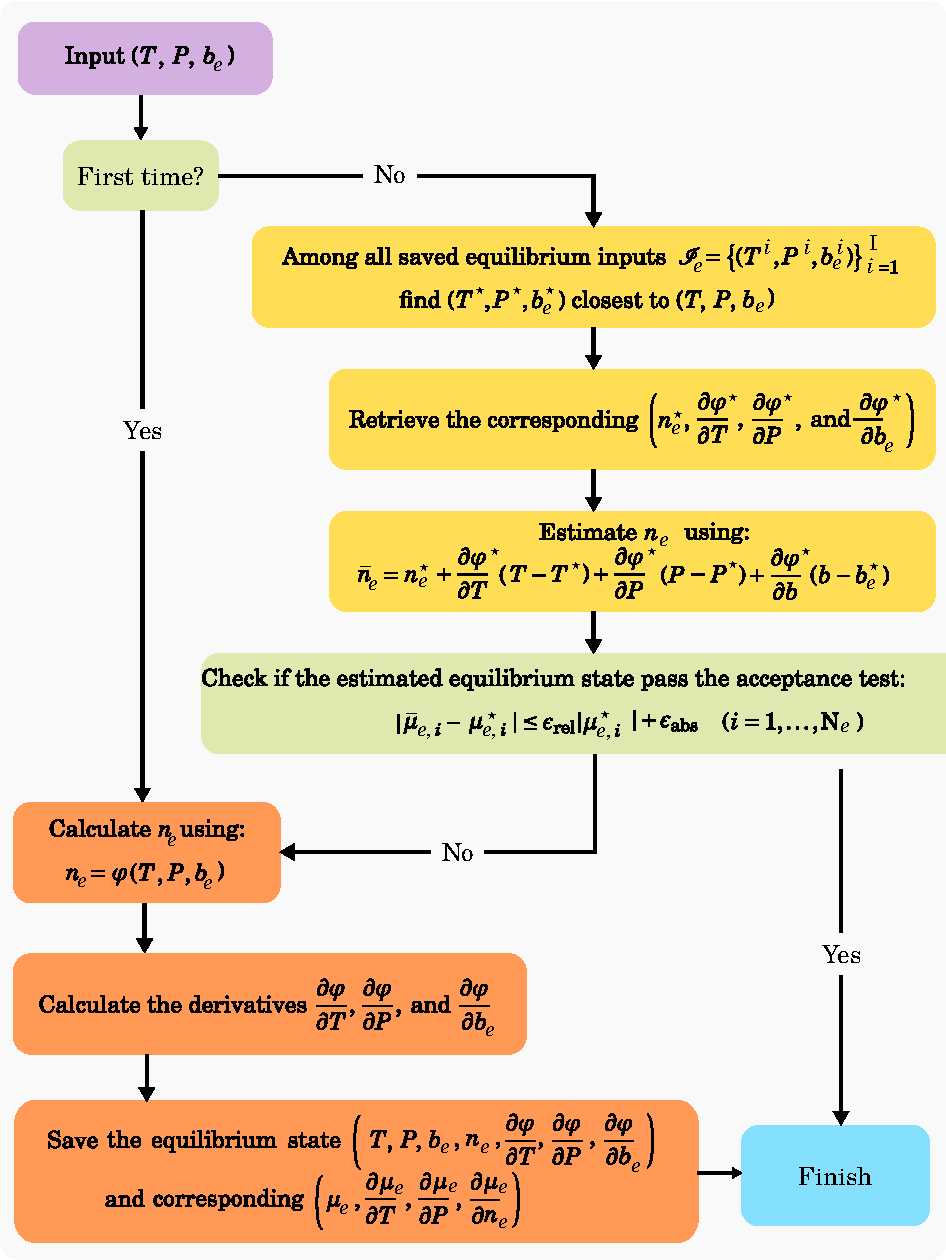
\includegraphics{figures/method/algorithm-flowchart-for-equilibrium}
\par\end{centering}
\caption{\label{fig:algorithm-diagram-equilibrium}
Diagram of the smart chemical equilibrium algorithm.}
\end{figure}

\begin{figure}
\begin{centering}
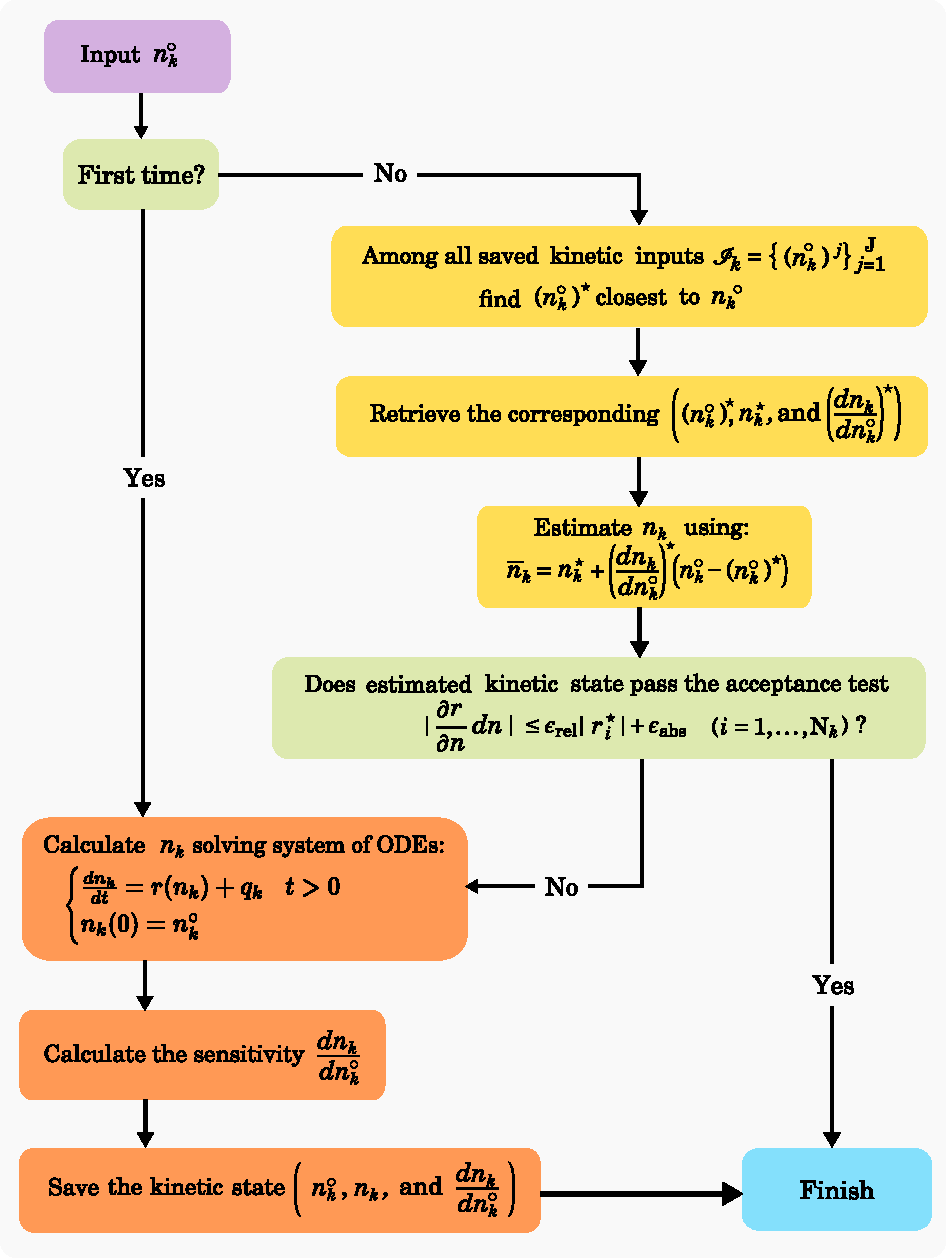
\includegraphics{figures/method/algorithm-flowchart-for-kinetics}
\par\end{centering}
\caption{\label{fig:algorithm-diagram-kinetics}
Diagram of the smart chemical kinetics algorithm.}
\end{figure}

%---------------------------------------------------------------------------------------------------%
The smart chemical equilibrium / kinetics algorithm proposed here is capable of remembering past 
chemical speciation calculations with corresponding sensitivity derivatives, using them to quickly 
and accurately estimate new equilibrium / kinetics states. 
%
The flowchart in Figure~\ref{fig:algorithm-diagram-equilibrium} illustrates the main steps of the 
algorithm focused on equilibrium species. At a very beginning, it solves the GEM problem 
Eq.~(\ref{eq:gem-problem}), which is represented by the computationally expensive equilibrium 
function~$\varphi$ Eq.~(\ref{eq:equilibrium-func}). Once this is done, the following information is 
saved for future fast and accurate predictions of equilibrium states, where the input conditions are 
relatively close to the one just recorded (i.e., learned):
%
\begin{itemize}
\item input conditions $(T, P, b_e)$;
\item corresponding calculated equilibrium amounts of species $n$;
\item sensitivity derivatives of the calculated equilibrium state: 
$\partial\varphi/\partial T$, $\partial\varphi/\partial P$, and $\partial\varphi/\partial b_e$;
\item derivatives of the chemical potentials 
$\partial\mu/\partial T$, $\partial\mu/\partial P$, and $\partial\mu/\partial n_e$.
\end{itemize}
%
See \citet{Leal2017} for a description of how to accurately calculate
these sensitivity and thermodynamic property derivatives.

%---------------------------------------------------------------------------------------------------%
Next time, when the algorithm is asked to solve a new equilibrium problem, it first does so by 
searching for the closest $(T,P,b_e)^{\star}$ to the given $(T,P,b_e)$ among all saved equilibrium 
input conditions in $\mathcal{I}_e$. Once the search is concluded, the previously calculated
potentially suitable equilibrium state is used to estimate the new equilibrium state using 
Eq.~(\ref{eq:smart-estimate}).
%---------------------------------------------------------------------------------------------------%
Finally, it remains to check if the estimated equilibrium state is accurate enough, using the 
acceptance test defined by Eq.~(\ref{eq:acceptance-test-mu}). If the test succeeds, then the 
speciation calculation ends. Otherwise, a complete chemical equilibrium calculation at $(T,P,b)$ is 
performed using GEM algorithm $n_e=\varphi(T,P,b_e)$. It is followed by similar derivative evaluation 
operations, as presented above, when the smart equilibrium algorithm was invoked for the first time.

\sveta{
%---------------------------------------------------------------------------------------------------%
The smart algorithm for kinetically controlled reactions is presented with the flowchart in 
Figure~\ref{fig:algorithm-diagram-kinetics}. It begins with integrating the system of ODEs 
Eq.~(\ref{eq:kinetics}) for the reconstruction of kinetic species. After that or simultaneously, 
the sensitivity matrix $\partial {n_k}/ \partial {n^\circ_k}$ is calculated. Once this information is 
collected, it is saved for future fast and accurate predictions of kinetic states, where the input 
conditions are relatively close to the one just stored (i.e., learned):
%
\begin{itemize}
\item input conditions $n^\circ_k$;
\item corresponding calculated amounts of kinetic species $n_k$;
\item sensitivity derivatives of the calculated kinetic state ${\partial n_k} / {\partial n^\circ_k}$;
\item properties of the corresponding chemical state, such as chemical rates $r$ and the composition 
of equilibrium species $n_e$.
\end{itemize}
%---------------------------------------------------------------------------------------------------%
Next time, when the algorithm needs to solve a new kinetic path, it first retrieves the closest 
$(n^\circ_k)^\star$ to the given $n^\circ_k$ among all saved kinetic initial conditions in 
$\mathcal{I}_k$. Next, the previously calculated potentially suitable kinetic state ${n_k}^\star$ is 
used as a reference to estimate the new kinetic state using Eq.~\eqref{eq:smart-estimate-kinetics}.
In the end, it remains to control whether the estimated kinetic state $\bar{n}_k$ satisfies the 
variational acceptance criterion defined by Eq.~\eqref{eq:acceptance-test-rates}. If this inequality 
is satisfied, then the calculation ends. Otherwise, complete numerical integration with the initial 
state $n^\circ_k$ is performed using the system Eq.~\eqref{eq:kinetics}. It is followed by the
evaluation of sensitivities as discussed-above, when the smart equilibrium algorithm was invoked 
for the first time.
}

%---------------------------------------------------------------------------------------------------%
\section{Results\label{sec:Results}}

\sveta{
We present here an example of using the smart chemical equilibrium / kinetics algorithm in a 
reactive transport simulation and show how its performance and precision compare to the use of a 
conventional chemical equilibrium / kinetics algorithms, based on either the Gibbs energy 
minimization for equilibrium species \citep{Leal2016a,Leal2017} or numerical integration for 
kinetically controlled ones \citep{Leal2017d}. Moreover, we demonstrate the results of coupling 
\texttt{Reaktoro} to an open-source finite element library \texttt{Firedrake} that is used to model 
transport after the operator-splitting of the reactive transport. For details on how we solve the 
reactive transport equations, see Appendix~\ref{sec:Reactive-Transport-Equations}.
}

\subsection*{Reactive Transport Problem\label{subsec:Reactive-Transport-Problem}}

%---------------------------------------------------------------------------------------------------%
The reactive transport modeling example carried out in this work is illustrated in 
Figure~\ref{fig:illustration-reactive-transport-model}. Here, the initial mineral composition of 
the horizontal porous rock column consists of 98\%$_{{\rm vol}}$ SiO$_{2}$(quartz) and 
2\%$_{{\rm vol}}$ CaCO$_{3}$(calcite), with an initial porosity of 10\% i.e., $\phi_{L} = 0.1$
where $\phi_{L}$ is a porosity at the cell on the inflow boundary. The resident 
fluid is a 0.70~molal~NaCl brine in equilibrium with the rock minerals (our calculated equilibrium 
state indicates a pH of about 9.2). The aqueous fluid injected on the left side of this rock 
column is the result of mixing 1~kg of water with 0.90~moles of NaCl, 0.05~moles of MgCl$_{2}$,
0.01~moles of CaCl$_{2}$, and 0.75~moles of CO$_{2}$. This amount of CO$_{2}$ is enough to bring 
the aqueous fluid close to CO$_{2}$ saturation at 100 bar, and thus in an acidic state, with a 
calculated pH of~3.05. The temperature and pressure of both resident and injected fluids
are 60~°C and 100~bar, respectively. The simplified reactive transport modeling assumes a constant 
fluid pore velocity (set in each cell) of $\boldsymbol{v}=\unit[1]{m/week}$ 
($\unit[5.95\cdot10^{-6}]{m/s}$) and the same diffusion coefficient $D=\unit[10^{-9}]{m^{2}/s}$ 
for all fluid species. %The longitudinal dispersivity is estimated as $D \, \phi\,/\,\boldsymbol{v}$, 
%which in this case is 100 times less than the usually accepted dispersivity of $10^{-3}$ m. 
\sveta{
Considered 1~m rock is discretized by the column mesh with 100~cells. The reactive transport 
simulation runs with 10`000 steps of uniform time step of 30~min, which results in 1'000'000 
chemical kinetics and equilibrium evaluations.
}

\begin{figure}
\begin{centering}
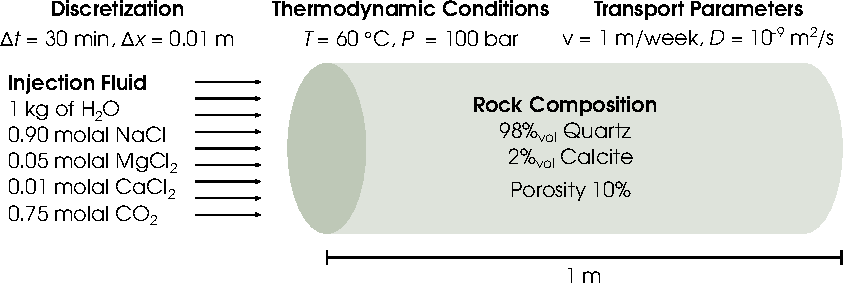
\includegraphics[width=0.7\textwidth]{figures/equilibrium/transport-scheme}
\par\end{centering}
\caption{\label{fig:illustration-reactive-transport-model}Illustration of
 reactive transport modeling along a one-dimensional rock core, including
some details on the injection fluid and rock composition, transport
parameters, and numerical discretization.}
\end{figure}


\subsection{Smart algorithm for chemical equilibrium, Pitzer activity model \label{subsec:part-1}}

%---------------------------------------------------------------------------------------------------%
In the chemical model part, the activity coefficients of the aqueous species are calculated using
the Pitzer model \citep{Pitzer1973}, formulated by \citet{Harvie1984}, except for the aqueous 
species CO$_{2}$(aq), for which the \citet{drummond1981boiling} model is applied. The standard 
chemical potentials of the species are calculated using the equations of state of 
\citet{Helgeson1974,Helgeson1978,Tanger1988,Shock1988} and \citet{Shock1992}. The database file 
\texttt{slop98.dat,} from the software SUPCRT92 \citep{Johnson1992}, is used to obtain corresponding
parameters. The equation of state of \citet{Wagner2002} is chosen to compute the density of water and 
its temperature and pressure derivatives. These prerequisites yield the system of \emph{36~chemical 
species} with \emph{4~phases} and \emph{9~chemical elements}. First, we neglect the dissolution and 
precipitation kinetics of both calcite and dolomite minerals (i.e., the local equilibrium assumption 
is employed). This way, we aim to assess how accurate the smart chemical equilibrium predictions are 
when phase transitions occur (e.g., when calcite fully dissolves and when dolomite starts to 
precipitate). 
%
\begin{figure}[!th]
\begin{centering}
\subfloat[]{{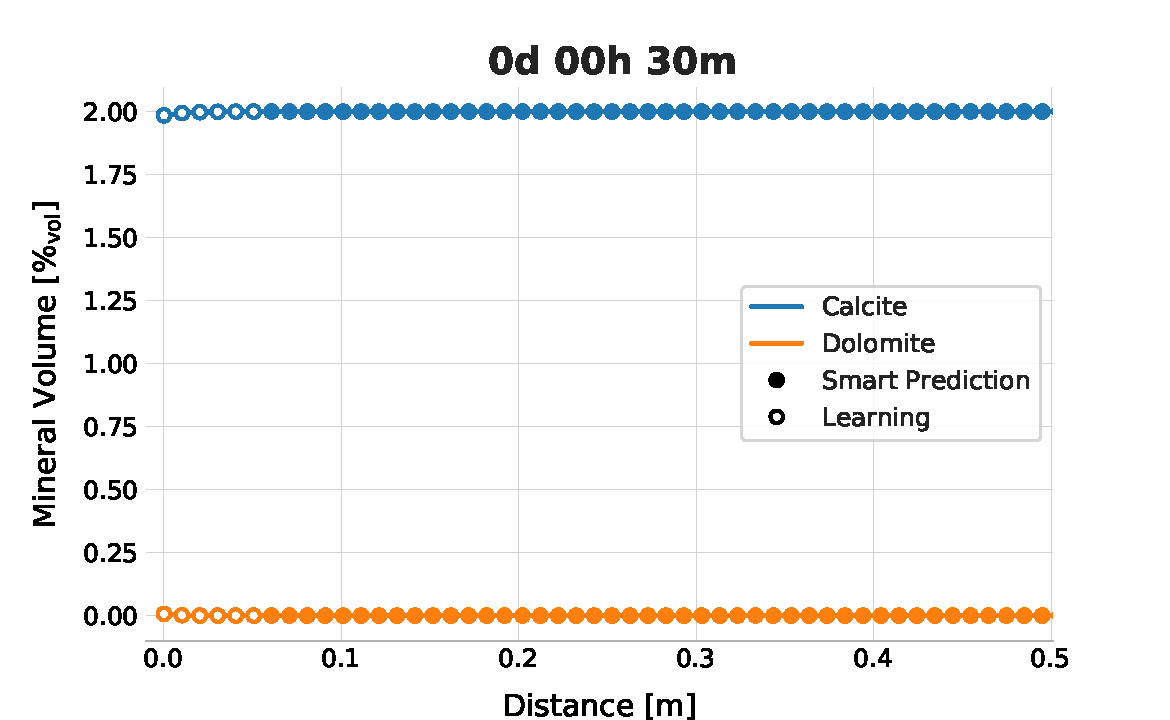
\includegraphics[width=0.45\textwidth, 
trim={0 0 1.5cm 0.5cm},clip]{figures/equilibrium/calcite-dolomite-1} 
\label{fig:calcite-dolomite-1}}}
\subfloat[]{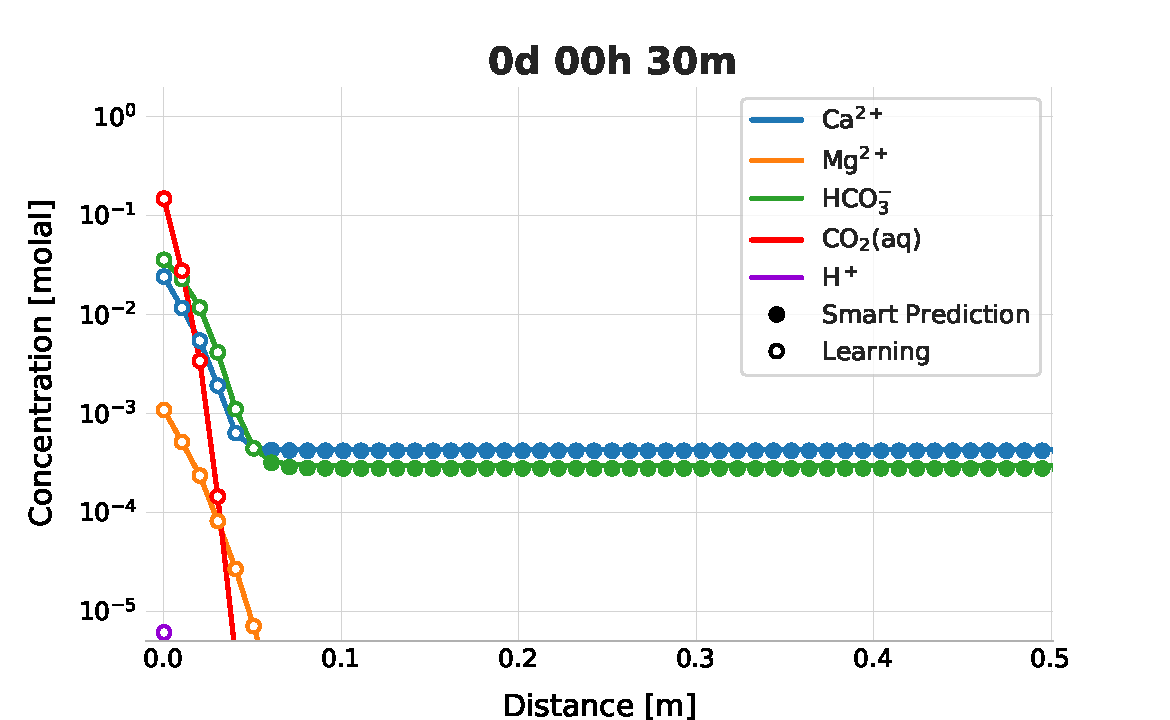
\includegraphics[width=0.45\textwidth, 
trim={0 0 1.5cm 0.5cm},clip]{figures/equilibrium/aqueous-species-1}
\label{fig:calcite-dolomite-2}}\\[-10pt]
\subfloat[]{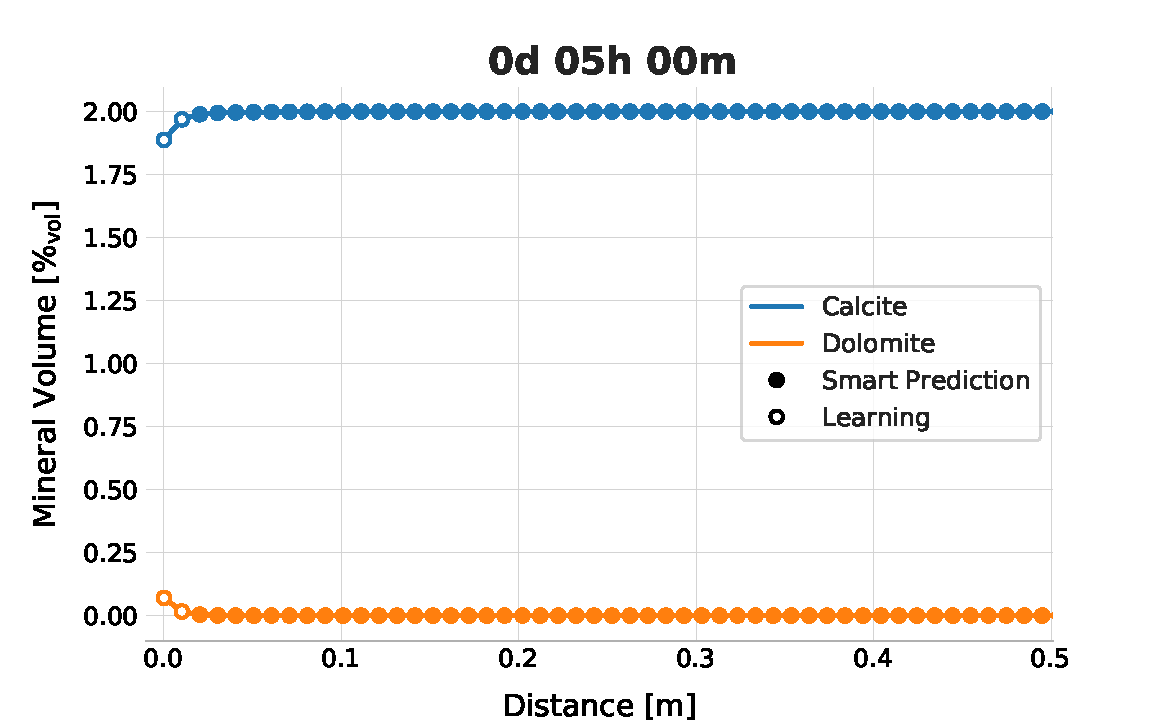
\includegraphics[width=0.45\textwidth, 
trim={0 0 1.5cm 0.5cm},clip]{figures/equilibrium/calcite-dolomite-10}
\label{fig:calcite-dolomite-3}}
\subfloat[]{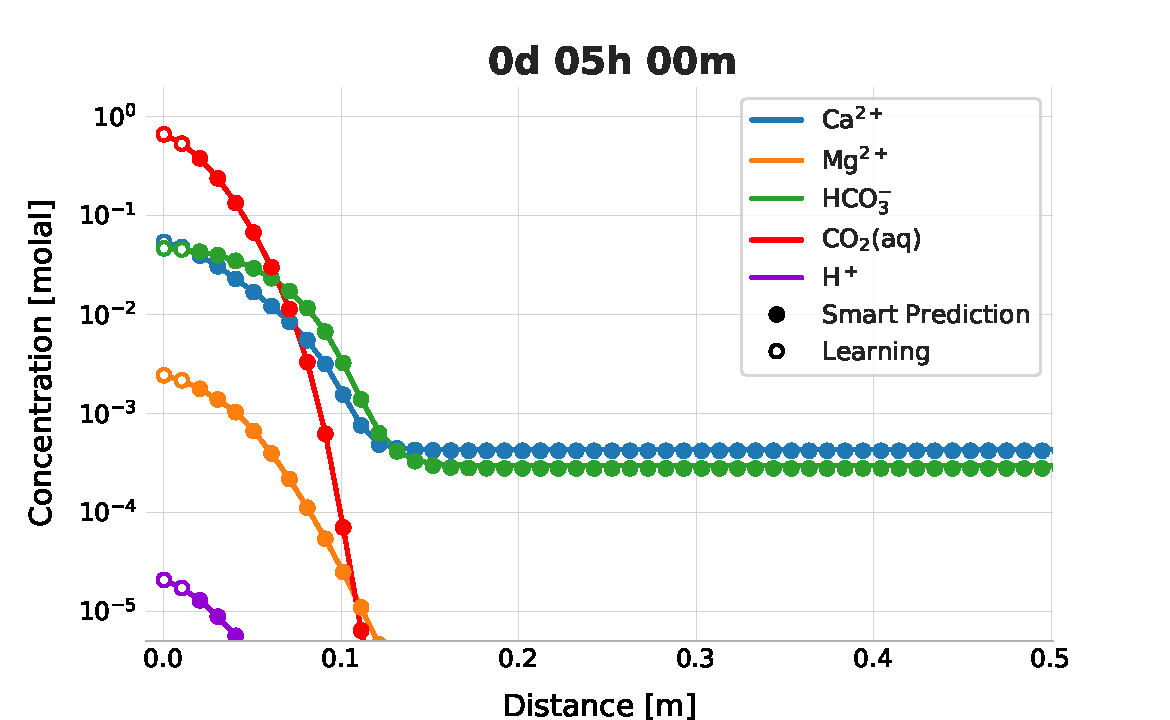
\includegraphics[width=0.45\textwidth, 
trim={0 0 1.5cm 0.5cm},clip]{figures/equilibrium/aqueous-species-10}
\label{fig:calcite-dolomite-4}}\\[-10pt]
\subfloat[]{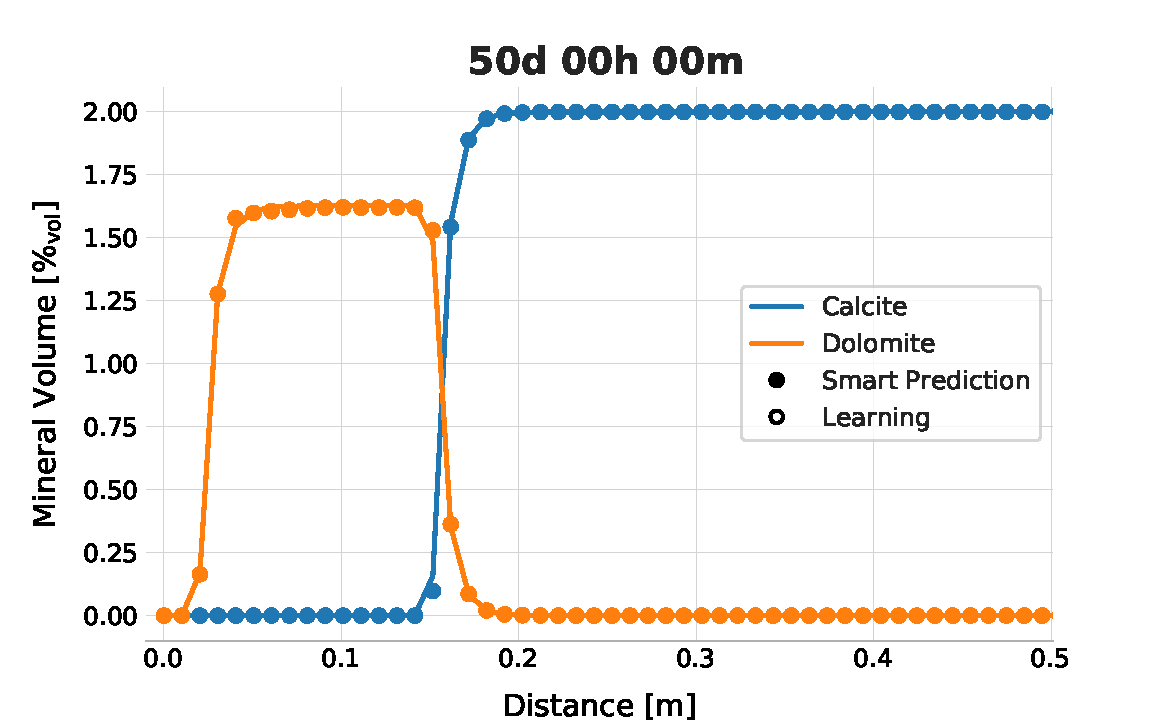
\includegraphics[width=0.45\textwidth, 
trim={0 0 1.5cm 0.5cm},clip]{figures/equilibrium/calcite-dolomite-2400}
\label{fig:calcite-dolomite-5}}
\subfloat[]{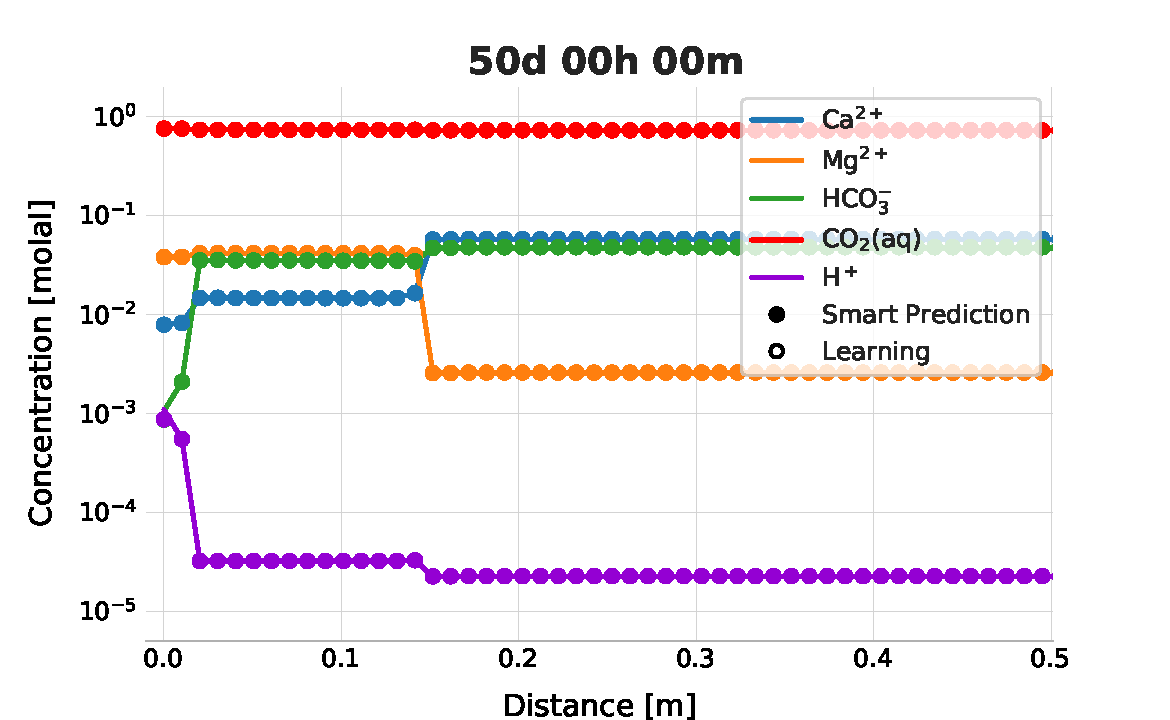
\includegraphics[width=0.45\textwidth, 
trim={0 0 1.5cm 0.5cm},clip]{figures/equilibrium/aqueous-species-2400}
\label{fig:calcite-dolomite-6}}
\par\end{centering}
\caption{\label{fig:calcite-dolomite} 
The volume percent ($\%_{{\rm vol}}$) of the minerals calcite and dolomite along the horizontal 
rock core as well as the concentrations of selected aqueous species (molal) at three different times: 
30~minutes, 5~hours, and 50~days (after 1, 10, and 2400~time steps of 30~minutes each, respectively). 
The \emph{solid lines} correspond to the results of the reactive transport simulation provided by 
conventional chemical equilibrium calculations based on full Gibbs energy minimization calculations 
performed in every cell of each time step. The circles ${\rm (}\bullet{\rm )}$ and 
${\rm (}\circ{\rm )}$ correspond to the values generated by the smart chemical equilibrium 
calculations. \emph{Solid circles} ${\rm (}\bullet{\rm )}$ indicate those cells, where successful
fast and accurate smart equilibrium predictions were preformed successfully. The 
\emph{empty circles} ${\rm (}\circ{\rm )}$ depict the cells, where full Gibbs energy minimization 
calculations were required and where, thus, \emph{on-demand learning} occurred.}
\end{figure}

%---------------------------------------------------------------------------------------------------%

\subsubsection{Smart Prediction Analysis \label{subsec:Performance-and-Accuracy}}
%
Figure~\ref{fig:calcite-dolomite} demonstrates the accuracy of the smart algorithm by comparing its 
results to the reference values generated by the conventional approach. In particular, it depicts the 
volume of minerals calcite, CaCO$_{3}$, and dolomite, CaMg(CO$_{3}$)$_{2}$ (left), as well as 
the concentrations of aqueous species Ca$^{2+}$(aq), Mg$^{2+}$(aq), HCO$_{3}^{-}$(aq), CO$_{2}$(aq), 
and H$^{+}$(aq) (right) along the horizontal rock column at three different simulation times: 
30~minutes, 5~hours, and 50~days. As calcite dissolves, Ca$^{2+}$(aq) ions are released into 
the aqueous solution, then reacting with the incoming Mg$^{2+}$(aq) ions from the left boundary 
to precipitate dolomite. After 30~minutes of injecting the CO$_{2}$-saturated brine (i.e., after a 
single time step), one observes a slight dissolution of calcite and corresponding precipitation of 
dolomite. 
%
The injected CO$_{2}$-saturated brine increases the local concentrations of carbolic species, 
CO$_{2}$(aq) and HCO$_{3}^{-}$(aq). The local concentrations of ions Ca$^{2+}$(aq) increases as a 
result of CaCO$_{3}$ dissolution. The precipitated dolomite, however, is gradually dissolved, as 
the injection of the acidic CO$_{2}$-saturated fluid continues. This can be seen in 
Figure~\ref{fig:calcite-dolomite} (bottom, left), in the very left region of the rock core, where 
neither calcite nor dolomite are present after 50~days of continuous fluid injection. At the same 
time, after 50~days of fluid injection (i.e., after 2400~time steps), the Mg$^{2+}$(aq) concentration 
drops sharply between core distances 0.1~m and 0.2~m, which is exactly where dolomite is currently 
precipitating. Moreover, in the same region Ca$^{2+}$(aq) concentration locally jumps as calcite 
dissolves.
%---------------------------------------------------------------------------------------------------%

We observe in Figure~\ref{fig:calcite-dolomite} that the use of the smart chemical equilibrium 
algorithm \emph{does not} compromise accuracy during the simulation. In this figure, the solid 
circles ${\rm (}\bullet{\rm )}$ represent a successful smart prediction of an accurate equilibrium
state at that cell position and time step, whereas the empty circles ${\rm (}\circ{\rm )}$ represent 
a failed attempt in this respect. The latter happens because of the absence of a previously solved 
chemical equilibrium problem similar enough to the new one. The empty circles ${\rm (}\circ{\rm )}$ 
also denote cells at which an on-demand learning operation was triggered, resulting in GEM 
calculation (that would be done anyway if the smart equilibrium algorithm was not used). These 
on-demand learning operations are triggered in different mesh cells, either on the same or different 
time steps. We remark that the current implementation of the algorithm does not rely on any spatial 
or temporal information, although this could be explored for faster search operations in the future.
%---------------------------------------------------------------------------------------------------%

From Figure~\ref{fig:calcite-dolomite}, we also can see that during the first time step of 
the simulation (30~minutes), the smart equilibrium algorithm was able to accurately estimate the 
equilibrium states in most mesh cells (see the solid circles $\bullet$). In other words, the 
algorithm learned enough distinct chemical equilibrium problems on a few upstream cells (near
the left boundary), which then could be successfully used for quick and accurate estimates for the 
rest of the cells downstream. To be precise, injecting the reactive fluid inside the rock core 
promotes strong compositional changes in both resident fluid and rock minerals. Because
of this, during the first time step, the algorithm requires \emph{on-demand learning} in 6 cells 
next to the left boundary (see the empty circles $\circ$ in Figure~\ref{fig:calcite-dolomite}). 
As the perturbation fronts move down the rock core, additional learning is performed as needed 
to fulfil a given accuracy criterion; here $\epsilon_{{\rm rel}}=10^{-1}$ and 
$\epsilon_{{\rm abs}}=10^{-8}$ are 
used in Eq.~(\ref{eq:acceptance-test-mu}). As seen in Figure~\ref{fig:calcite-dolomite} (after 5h, 
or 10~time steps), 2~cells required a full and expensive chemical equilibrium calculation to both 
ensure accuracy and enable on-demand learning. 
\sveta{
We also point out that after the certain amount of the time steps, trainings that are expected to be 
triggered at the cells, where a change of phases is happening, are not occurring any more. The 
algorithm has already gathered enough information about the system on the first time steps (while 
dolomite just started its precipitation and calcite its dissolution) so it does not have to learn 
further down the road.}
%---------------------------------------------------------------------------------------------------%

\begin{figure}[!t]
\begin{centering}
\subfloat[]{{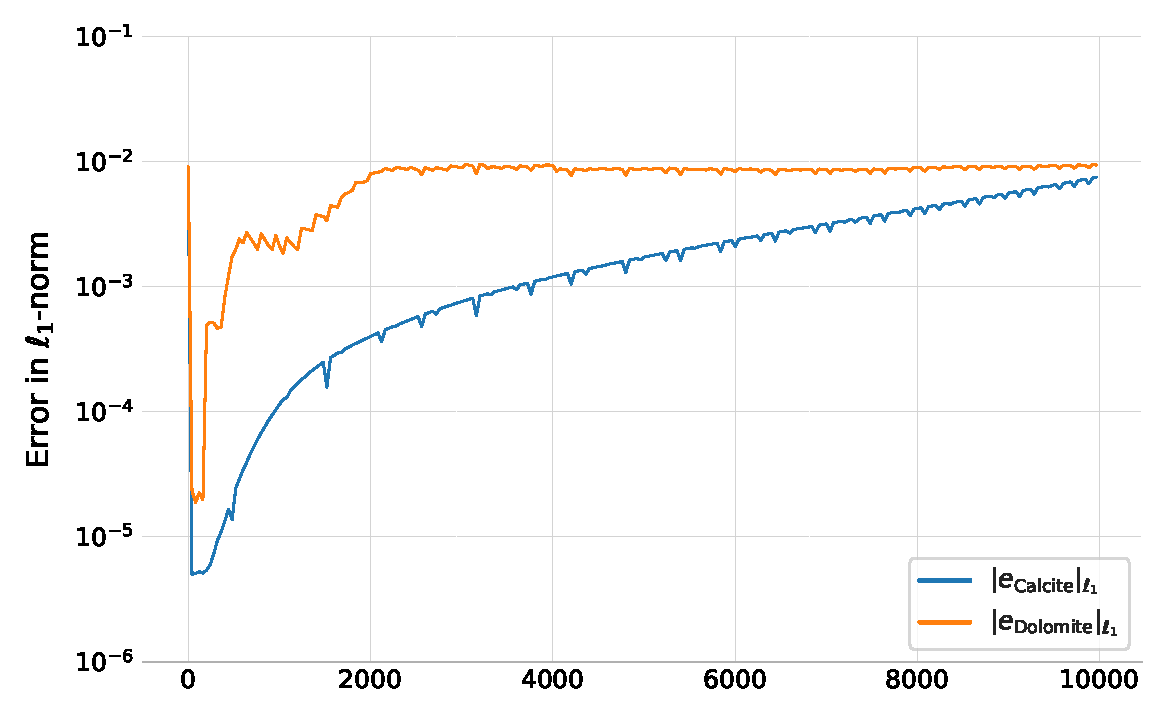
\includegraphics[width=0.48\textwidth, 
trim={0 0 1cm 0},clip]{figures/equilibrium/errors-calcite-dolomite-l1} \label{fig:error-1}}}
\subfloat[]{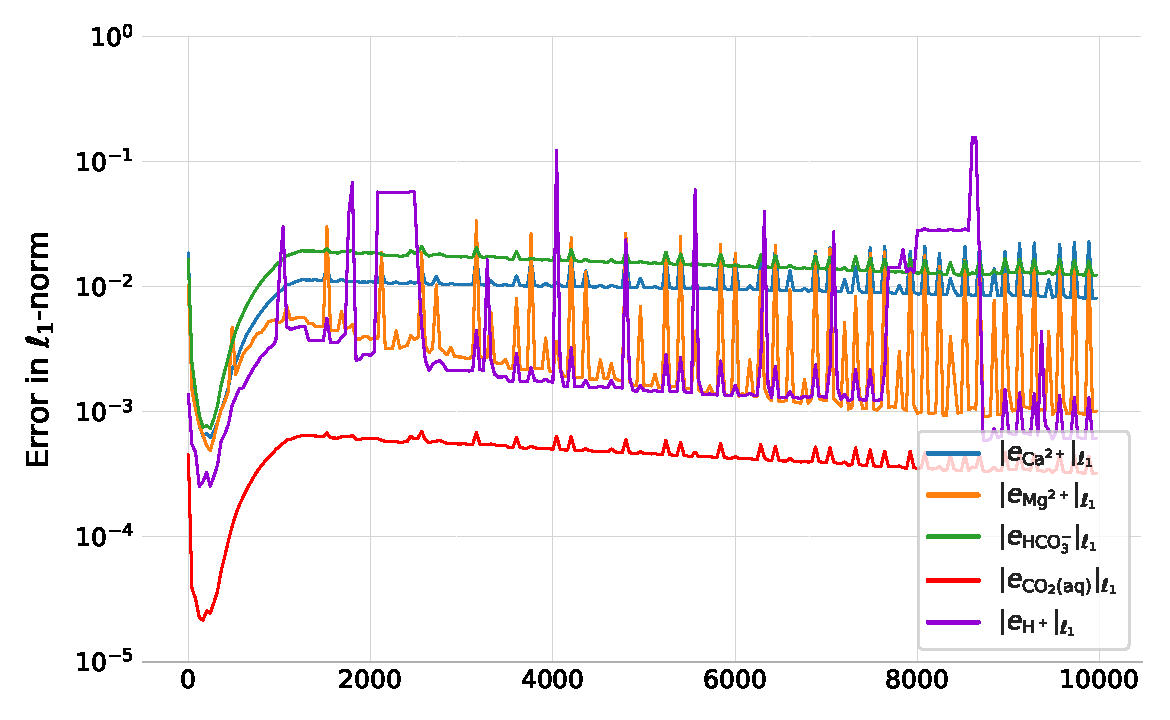
\includegraphics[width=0.48\textwidth, 
trim={0 0 1cm 0},clip]{figures/equilibrium/errors-aqueous-l1}
\label{fig:error-2}} \\
\subfloat[]{{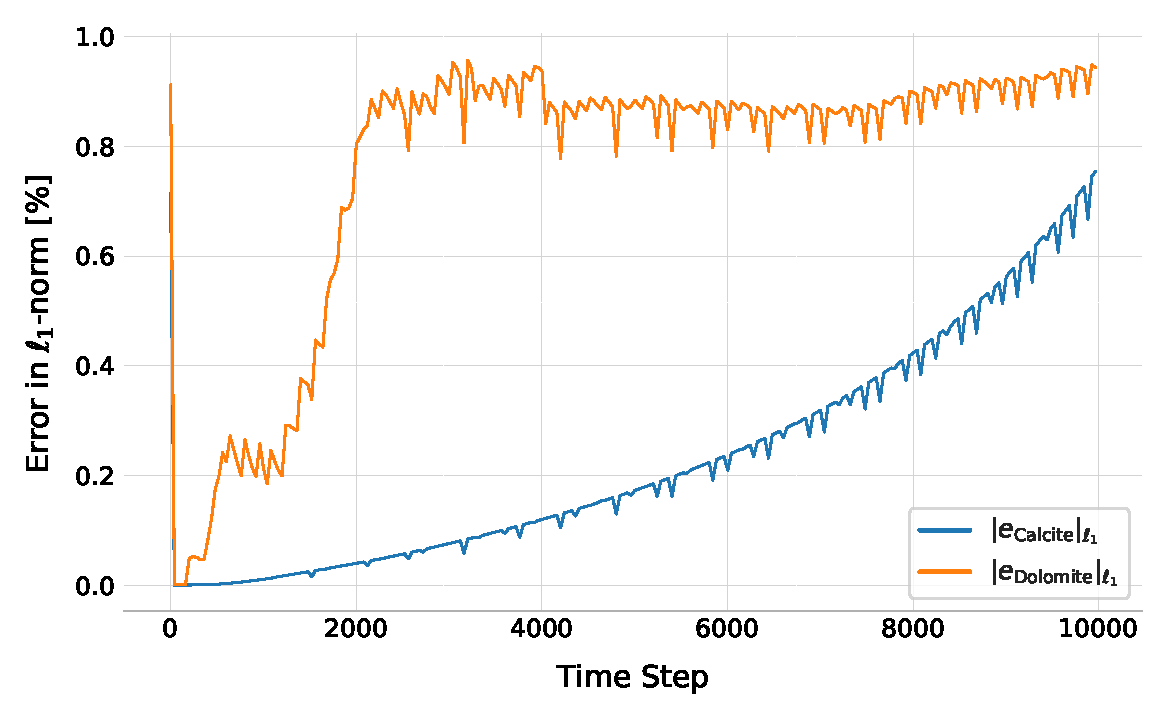
\includegraphics[width=0.48\textwidth, 
trim={0 0 1cm 0},clip]{figures/equilibrium/errors-calcite-dolomite-l1-percent} \label{fig:error-3}}}
\subfloat[]{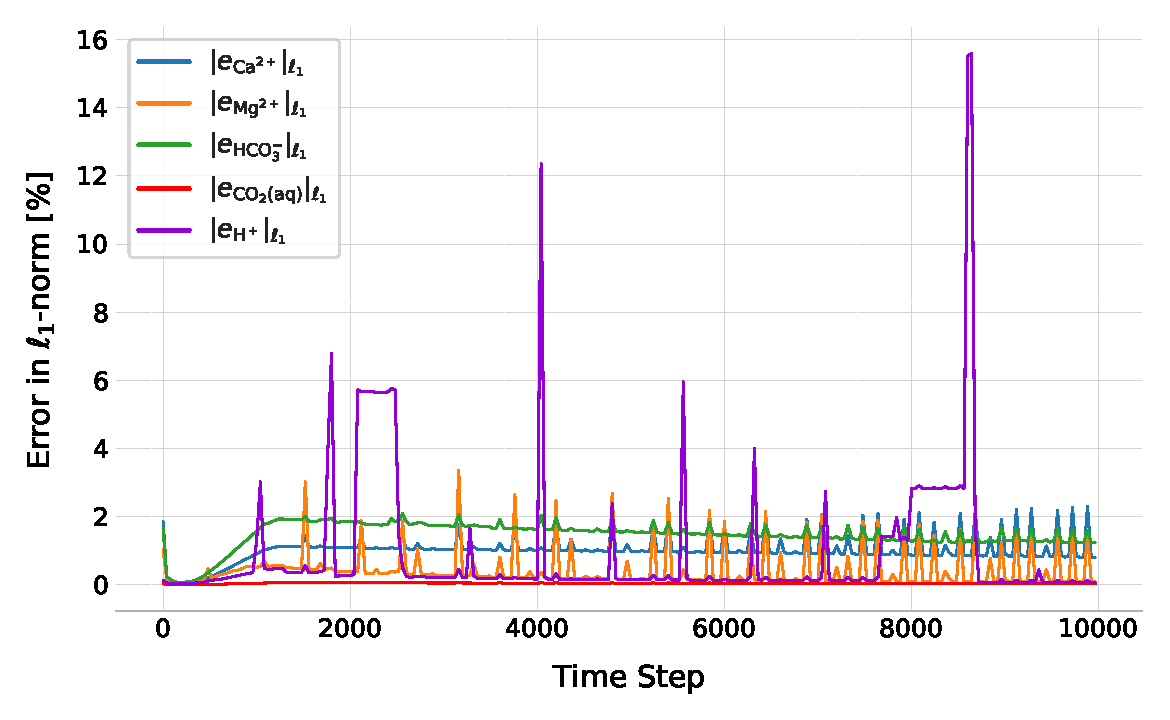
\includegraphics[width=0.48\textwidth, 
trim={0 0 1cm 0},clip]{figures/equilibrium/errors-aqueous-l1-percent}
\label{fig:error-4}}
\par\end{centering}
\caption{\label{fig:error}
Error between results provided by the smart algorithm and reference values provided 
by the conventional approach. The $\ell_1$-norm of the error in the calcite and dolomite (left) 
and in aqueous species (right).}
\end{figure}
\sveta{
%---------------------------------------------------------------------------------------------------%
The percentage of the error measured in $\ell_1$-norm is illustrated in Figure \ref{fig:error}. 
We see that the $\ell_1$-norm of the error in the calcite and dolomite minerals lies in the range 
$[10^{-5}, 10^{-2}]$, whereas the error in aqueous species might get an order higher 
$[10^{-5}, 10^{-1}]$. The latter can be related to a slight delay in the smart algorithm to reproduce 
sharp changes in ions concentrations. This yields that the uncertainty in minerals' volumes is bounded 
by 1~\% (i.e., $|e_{\rm CaCO_3}|_{\ell_1}$ = 0.76 \% and $|e_{\rm CaMg(CO_3)_2}|_{\ell_1}$ = 0.96 \%).
The inaccuracies of the aqueous concentrations reproduced by the on-demand learning lie in a similar 
range, i.e., $|e_{\rm pH}|_{\ell_1}$ = 0.62 \%, $|e_{\rm Ca^{2+}}|_{\ell_1}$ = 2.32 \%, 
$|e_{\rm Mg^{2+}}|_{\ell_1}$ = 3.76 \%, $|e_{\rm HCO_3^{-}}|_{\ell_1}$ = 2.53 \%, 
$|e_{\rm Ca^{2+}}|_{\ell_1}$ = 2.32 \%, $|e_{\rm CO_2(aq)}|_{\ell_1}$ = 0.08 \%, except the error in 
${\rm H}^{+}$ might get up to 10/16~\% in several cells throughout the simulation. 
}

\begin{comment}
max |e in pH|_l1 = 0.62 procent
max |e in calcite|_l1 = 0.76 procent
max |e in dolomite|_l1 = 0.96 procent
max |e in hcation|_l1 = 16.67 procent
max |e in cacation|_l1 = 2.32 procent
max |e in mgcation|_l1 = 3.76 procent
max |e in hco3anion|_l1 = 2.53 procent
max |e in cacation|_l1 = 2.32 procent
max |e in co2aq|_l1 = 0.08 procent
\end{comment}

\sveta{
\begin{figure}[!t]
\centering
\subfloat[Number of the on-demand learnings per time step]{
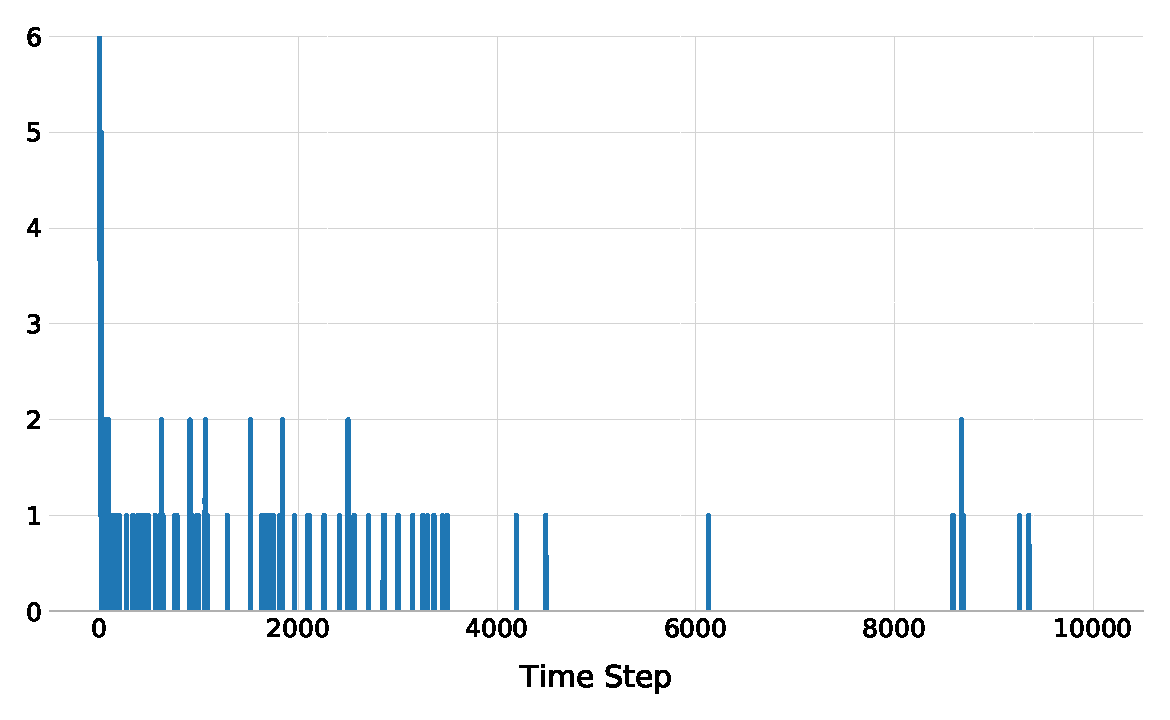
\includegraphics[width=0.6\textwidth]{figures/equilibrium/on-demand-learning-countings}
\label{fig:number-training-1}} \\
\subfloat[Total number of the on-demand learnings with respect to time]{
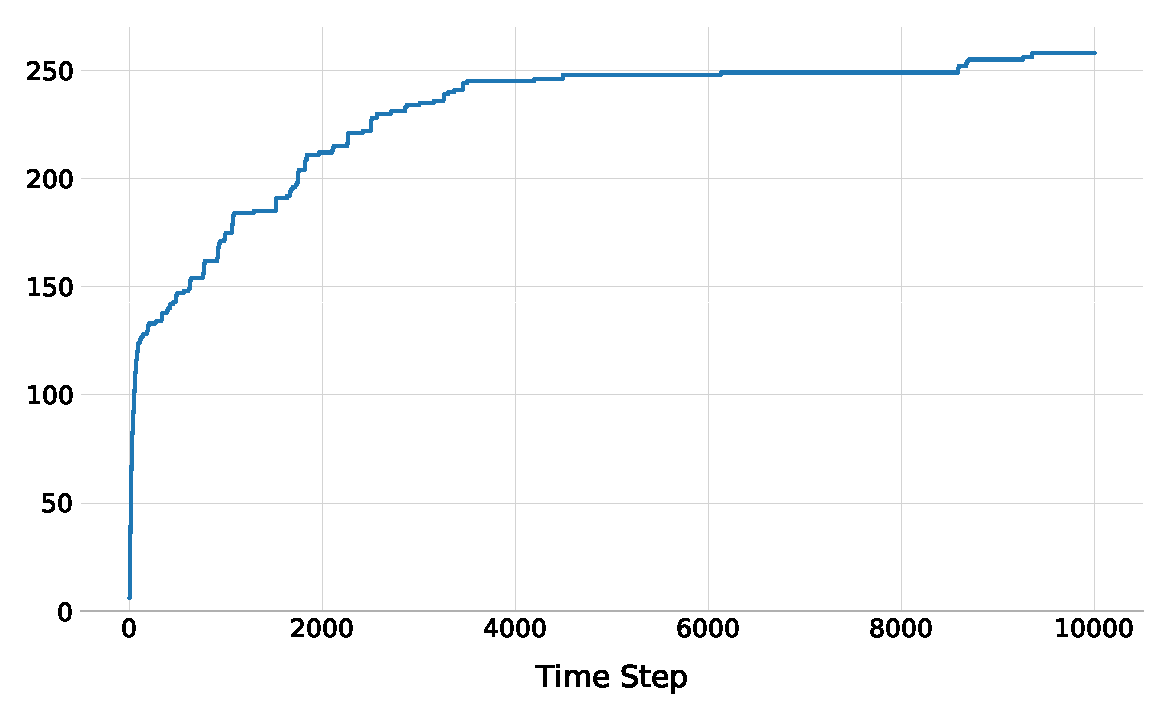
\includegraphics[width=0.6\textwidth]{figures/equilibrium/on-demand-learning-total}
\label{fig:number-training-2}}
\caption{\label{fig:number-training}
(a) Number of \emph{on-demand learning} operations triggered by the smart chemical equilibrium 
algorithm at each time step and (b) the accumulated number of cells, where full GEM problems were 
triggered during the reactive transport simulation. The simulation finished after 10'000 time steps 
and required thus the solution of 1'000'000 chemical equilibrium problems. Only 258 (or 0.03\%) of 
these were solved using GEM calculation; the majority (99.97\%) were quickly and accurately 
estimated with the smart chemical equilibrium algorithm.}
\end{figure}
}
%---------------------------------------------------------------------------------------------------%
Figure~\ref{fig:number-training} presents the number of on-demand learning operations (a) occurring 
per each time step and (b) accumulated during the reactive transport simulation. 
In Figure \ref{fig:number-training-2}, 
note rather high total number growth on the initial time steps, where the smart chemical equilibrium 
algorithm is actively learning new chemical states. \sveta{The latter corresponds to Figure 
\ref{fig:number-training-1}, where for the first reactive transport steps full Gibbs energy 
minimization calculations are needed to be performed in up to 6 cells out of 100 ones.}
%
This is the result of the incoming brine perturbing the fluid composition on the left side of the 
horizontal rock core. As time passes, the increment of total on-demand learning operations becomes 
very small, about 1~or 2~cells per time step. The latter can be observed on the top subplot in 
Figure~\ref{fig:number-training}). 
%
Eventually, the smart prediction algorithm becomes knowledgeable enough about the recurring 
equilibrium states in the simulation, so that it can quickly and accurately perform all subsequent
speciations without further learning, or with just a few occasional training acts. We remark that 
this result is specific to the reactive transport example investigated here. In a reactive transport 
problem with more heterogeneity, for example, one could expect somewhat more on-demand learning 
requirements. We plan to investigate this dependency in future work.

%---------------------------------------------------------------------------------------------------%
\begin{figure}[!t]
\begin{centering}
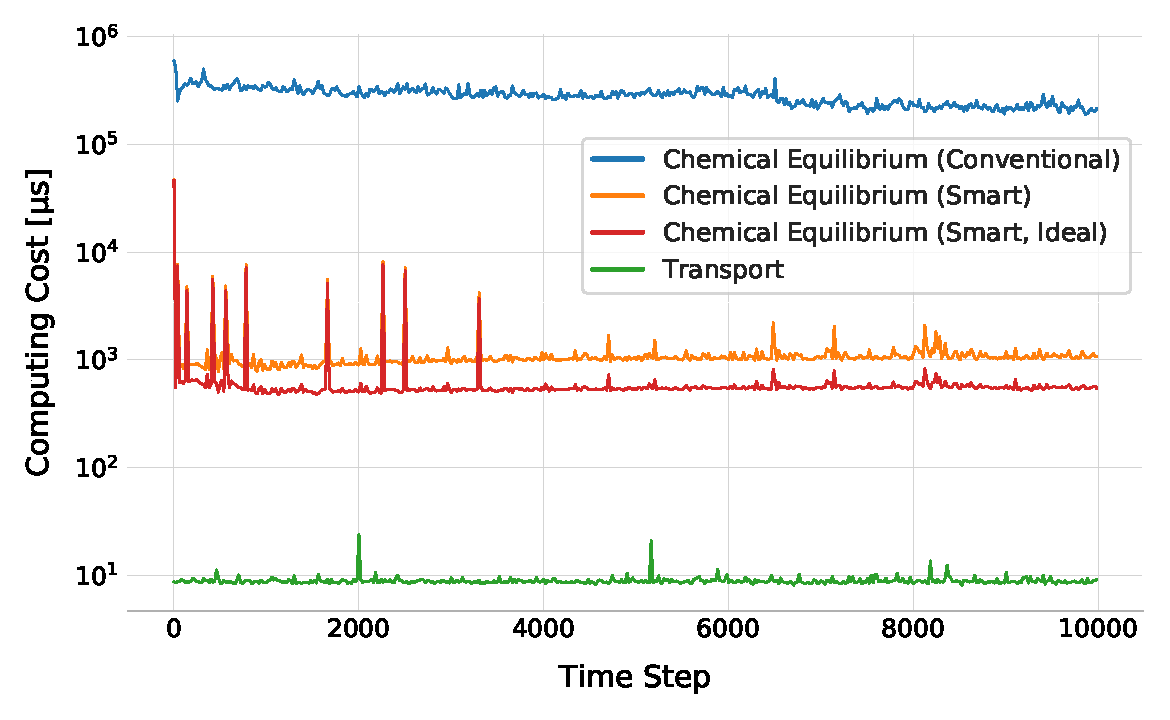
\includegraphics[width=0.7\textwidth]{figures/equilibrium/computing-costs-with-ideal}
\par\end{centering}
\caption{\label{fig:computational-cost}
Comparison of the computing costs (CPU time in microseconds) of transport, conventional, smart 
chemical equilibrium calculations, and so-called \emph{zero-search-cost} smart equilibrium 
calculations during each time step of the reactive transport simulation. The cost of equilibrium 
calculations per time step is the sum of the individual costs in each mesh cell,  whereas the cost 
of transport calculations per time step is the time required when solving the discretized algebraic 
transport equations. The zero-search-cost smart equilibrium calculation is the costs of on-demand 
learning algorithm excluding the costs for NN search.}
\end{figure}
%---------------------------------------------------------------------------------------------------%
Figure~\ref{fig:computational-cost} compares the computational cost at each time step of: 
\emph{(i)} conventional chemical equilibrium calculations, 
\emph{(ii)} smart chemical equilibrium calculations (or zero-cost-search smart equilibrium 
calculations), and \emph{(iii)} transport calculations. 
%
These costs are measured as CPU time in microseconds. For the equilibrium calculations, conventional
and smart, we show CPU time needed to calculate all equilibrium states across all mesh cells within 
the same time step. For the transport calculations, the cost is the time needed to solve the 
algebraic transport equations (we use direct Thomas algorithm for tridiagonal linear systems). 
\sveta{
As the name suggests, zero-cost-search smart equilibrium calculations are the costs of 
on-demand learning algorithm per each reactive transport time step excluding the costs of NN search.}
%---------------------------------------------------------------------------------------------------%
Figure~\ref{fig:computational-cost} confirms that the cost of conventional chemical equilibrium 
calculations can be orders of magnitude higher than the cost of transport calculations (about five 
orders of magnitude higher in this relatively simple reactive transport example). The figure also shows 
that the computational cost associated with chemical equilibrium calculations is drastically reduced 
using the smart equilibrium algorithm (by about three orders of magnitude when smart predictions are 
made in all mesh cells during a time step). We note that during the first time steps of the reactive
transport simulation, the CPU time spent on the smart equilibrium algorithm has relatively high spikes
in comparison to that after 4000~time steps. We observe for most of those spikes that the need of 
on-demand learning existed only in 1~to 2~cells (out of 100). After about half of the simulation time, 
the orange curve exhibits only few peaks, which correspond to only occasional learning acts, demanded 
by the acceptance test of the algorithm. 
\sveta{
The red line, corresponding to the zero-cost-search smart 
equilibrium calculations, indicates potential improvement in the CPU time of the on-demand learning 
algorithm once the costs of the reference point retrieval will be improved. Below, we consider 
several strategies to address the performance of look-up operations for already evaluated chemical 
states.
}

\subsubsection{Nearest Neighbor Search Analysis\label{subsec:Nearest-Neighbor-Search-Analysis-Equilibrium}}

%---------------------------------------------------------------------------------------------------%
As mentioned above, estimating an equilibrium state in a smart chemical equilibrium calculation 
requires a retrieval operation for the reference chemical state, which can be used in Taylor expansion. 
Currently, this search is performed among all currently recorded fully solved chemical equilibrium
problems, during the ongoing reactive transport simulation. It is needed to find the previously 
solved equilibrium problem whose input conditions are the closest (in the sense of Euclidean norm) 
to the input conditions of the new problem. Thus, the computing cost of the search operation 
increases as we perform more on-demand learning calculations because, at the end of each of them, 
a newly learned equilibrium state is stored.

\begin{figure}[!t]
\begin{centering}
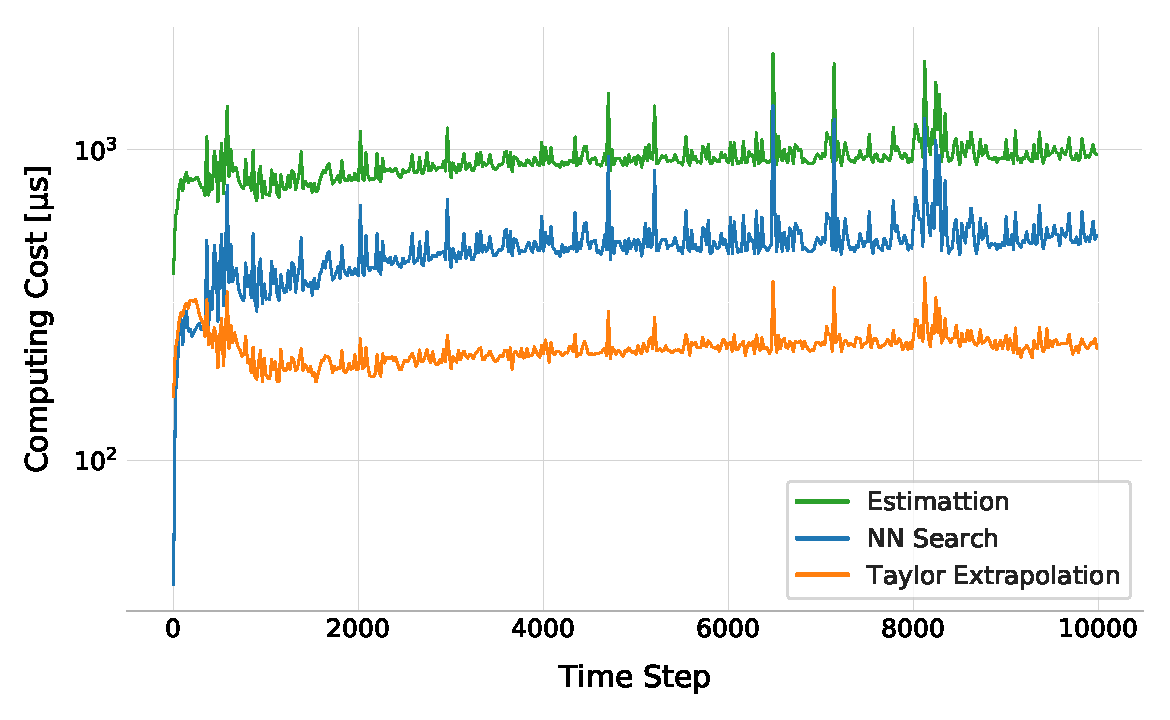
\includegraphics[width=0.7\textwidth]{figures/equilibrium/search-traylor-vs-total-learnings}
\par\end{centering}
\caption{\label{fig:search-traylor-vs-total-learnings}
%
The computing time for the total estimation, NN search operations, as more fully solved equilibrium 
problems are stored during the simulation. A comparison is made against the computing time required 
for the first-order Taylor expansion calculation, which is a small and fast matrix-vector 
multiplication with more or less constant cost throughout. }
\end{figure}

%---------------------------------------------------------------------------------------------------%
Figure~\ref{fig:search-traylor-vs-total-learnings} demonstrates this increase in search cost as more 
learned equilibrium problems are recorded during the reactive transport simulation (orange line). 
This time impacts directly to the general costs of the estimation step (green line). They are both 
compared to the cost of performing a first-order Taylor expansion calculation (a small and fast 
matrix-vector multiplication), which exhibits rather constant computing costs. This increase in 
search time eventually ceases and becomes constant, because the smart algorithm has already learned 
enough key chemical equilibrium problems to quickly estimate most (in some cases all) subsequent 
ones. 
%
However, should the problem contain more geologic and/or chemical complexity, this cost could 
continue to increase. This most certainly implies the importance of the use of the data structure 
(such as kd-tree or locally sensitive hashing tables) that would allow maintaining the costs of 
retrieval algorithm constant and amenable. 
%
\sveta{
To further improve search times, previously-stored learned problems could also be ranked 
so that those that have not had much use for quickly predicting new states are purged from the 
database eventually. The chemical state most often used for smart prediction will have a higher rank
that can define their order of processing during the retrieval step. To be precise, as soon as such 
reference state provides an accurate enough prediction, the search can be terminated and its costs 
would be optimized to remain negligible (compared to other costs in the simulation).
}

%---------------------------------------------------------------------------------------------------%
\begin{figure}[!t]
\begin{centering}
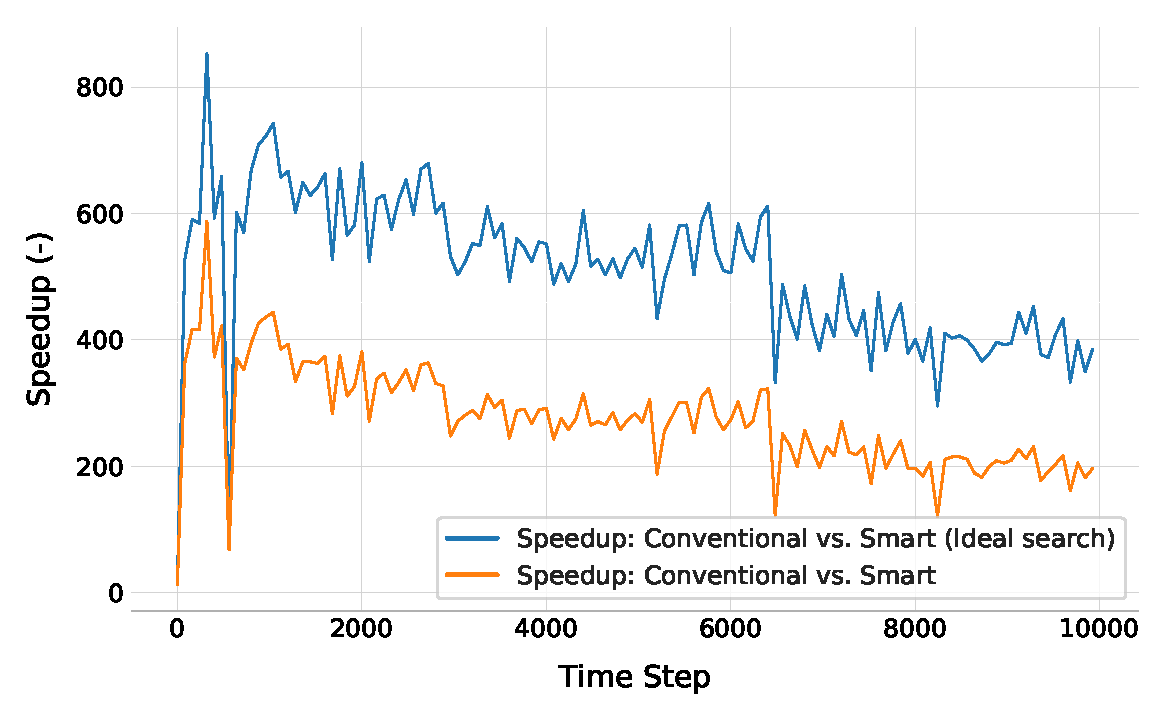
\includegraphics[width=0.7\textwidth]{figures/equilibrium/speedups}
\par\end{centering}
\caption{\label{fig:speedup-with-and-without-search-costs}
The speedup factor of chemical equilibrium calculations, at each time step of the simulation, 
resulting from the use of the on-demand learning acceleration strategy, employing a linear NN search 
(orange). A comparison is made with the speedup obtained by removing the computing time needed for 
the retrieval of the reference state (blue). The latter indicates an upper bound for the speedup 
upon improvement of the search algorithm.}
\end{figure}

%---------------------------------------------------------------------------------------------------%
\sveta{Let us consider the speedup at each time step of the reactive transport simulation, which is 
calculated as the ratio of the accumulated time needed for the conventional to the smart chemical 
equilibrium calculations across all cells in the mesh. It is depicted in Figure 
\ref{fig:search-traylor-vs-total-learnings} with an orange line.}
%
Considering a hypothetical ideal NN search algorithm, whose computing cost is zero, we have 
shown that the search operations contribute most to the computation cost of the smart chemical 
equilibrium method. This is the case, as the Taylor expansion calculation is fast (see Figure 
\ref{fig:search-traylor-vs-total-learnings} discussed above). By excluding the costs of the NN 
search (which we also refer to as ideal or zero-cost NN search algorithm) should yield an 
approximation of the upper bound of the speedup we expect to obtain (see blue line in Figure~\ref{fig:speedup-with-and-without-search-costs}). The speedup of our current implementation 
of the smart chemical equilibrium algorithm stabilizes at a value close to 200, whereas the ideal 
speedup is about 400. Thus, further research and improvements in this regard are needed further 
acceleration of the algorithm. 

\subsection{Smart algorithm for chemical kinetics, HKF activity model \label{subsec:part-2}}

Next, we consider the performance of smart chemical kinetics algorithm.
%---------------------------------------------------------------------------------------------------%
The on-demand learning for chemical equilibrium algorithm, discussed in the details in Subsection 
\ref{subsec:part-1}, can be used in the simulations of kinetically controlled species. 
We clarify the steps of the ODML algorithm for chemical kinetics for each reactive transport 
step $[t_k, t_{k+1}], k = 1, \ldots {\rm K}$ in Algorithm \ref{eq:kinetics-algorithm}.
%
\begin{comment}
\begin{itemize} 
\setlength{\itemsep}{0pt} \setlength{\parskip}{0pt}
\item Transport generates $n^\circ = [n^\circ_k; n^\circ_e]$ for all cells.
\item For each cell: 
\begin{itemize}
\setlength{\itemsep}{0pt} \setlength{\parskip}{0pt}
\item Evolve kinetics species $n_k$ by smart kinetics algorithm (see Figure \ref{fig:kinetics-algorithm}) 
using either {on-demand learning/training/full system of ODEs integration} (which corresponds to 
empty circles {\large $\fullmoon$}) or {prediction/estimation} (filled circles {\large $\newmoon$}).
\item Update equilibrium species $n_e$.
\end{itemize}
%
\item Combine the species amounts $n = [n_k; n_e]$.
\end{itemize}
\end{comment}

\begin{algorithm}[!t]
\small
\SetAlgoLined
\KwResult{species amounts $n$ at the step $[t_k, t_{k+1}], k = 1, \ldots, {\rm K}$}
  transport generates $n^\circ = [n^\circ_k; n^\circ_e]$ for all cells\;
 \For{each cell}{
  $\bullet$ evolve kinetics species $n_k$ by smart kinetics algorithm (see Figure \ref{fig:kinetics-algorithm}) 
  using either\\
    \qquad {on-demand learning/training/full system of ODEs integration} (empty circles {\large $\fullmoon$}) or \\
    \qquad {prediction/estimation} (filled circles {\large $\newmoon$})\;
  $\bullet$ update equilibrium species $n_e$\;
  $\bullet$ combine the species amounts $n = [n_k; n_e]$\;
 }
\caption{The ODML algorithm for chemical kinetics for $k$th reactive transport step.}
\label{eq:kinetics-algorithm}
\end{algorithm}
%
\begin{figure}[!t]
\begin{centering}
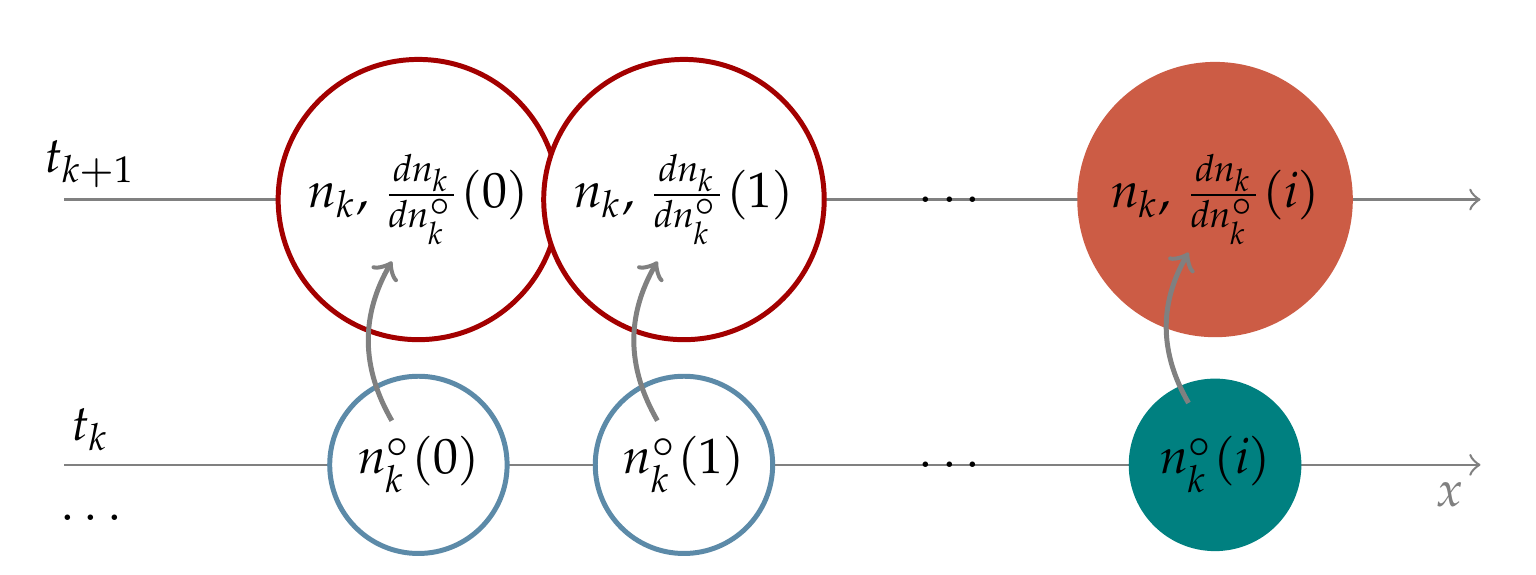
\includegraphics[width=0.6\textwidth]{figures/kinetics/algorithm.png}
\par\end{centering}
\caption{\label{fig:kinetics-algorithm}. 
The ODML algorithm for chemical kinetics on the reactive step $[t_k, t_{k+1}], k = 1, \ldots, {\rm K}$.}
\end{figure}

%---------------------------------------------------------------------------------------------------%
In the chemical model part, the activity coefficients of the aqueous species are calculated using
the HKF model extended Debye-H\"uckel model \citep{Helgeson1974a, Helgeson1974, Helgeson1976, 
Helgeson1981} for solvent water and ionic species, except for the aqueous 
species CO$_{2}$(aq), for which the \citet{drummond1981boiling} model is applied. The rest of the chemical
properties coincides with assumptions of Subsection \ref{subsec:part-1}. We assume dissolution kinetics 
for calcite, whereas dolomite is precipitating in equilibrium (using local equilibrium assumption). 
The considered reaction of calcite dissolution is 
%
$$\mbox{CaCO}_3(s) + {\rm H}^{+} \rightleftharpoons \mbox{Ca}^{2+} + \mbox{HCO}_3^{-}.$$
%
Rates of minerals' dissolution can be represented by the following function for the $m$th mineral
%
$$r_{m}(T,P,n):= \mathcal{A}_{m}(n_m)\sum^{\rm reactions}_{i} \mathcal{M}_{m,i}(T,P,n), 
\quad r_{m}:\mathbb{R}^{2+N} \rightarrow \ensuremath{\mathbb{R}},$$ where 
%
$\mathcal{A}_{m} := n_{m} \, \sigma_{m}$ is a \emph{surface area function} \big[$\mathrm{m^2}$\big] 
with the \emph{current molar amount} of the mineral $n_{m}$ \big[$\mathrm{mol}$\big] 
and the \emph{current specific reactive surface area} $\sigma_{m}$ \big[$\mathrm{{m^2}/{mol}}$\big]. 
%
Here, 
$$\mathcal{M}_{m,i} 
:= k_{m,i} \, {\rm sgn}(1-\Omega) \, |1-\Omega^{p_{i}}|^{q_{i}} 
\,\prod_{j} a_{j}^{\xi_{j}} \prod_{g} P_{g}^{\eta_{g}}$$
%
is the \emph{$i$th kinetic mechanism function} \big[$\mathrm{mol}/\mathrm{m^2 s}$\big], where 
$\Omega := {1}/{K_{m}}\prod_{i=1}^{N} \, a_{i}^{\nu_{i}}$ is the \emph{saturation index} 
defined via the product of activities with power of \emph{stoichiometric coefficient} $\nu_{i}$ of 
the $i$th ionic species and \emph{equilibrium constant} $K_{m}$. 
%
The $i$th \emph{rate constant} $k_{m,i}$ is defined by the \emph{Arrhenius equation} 
%
$$k_{m,i} := k_{m,i}^{\circ} \exp \Big[-\tfrac{E_{m,i}}{R}(\tfrac{1}{T}-\tfrac{1}{298.15})\Big],$$ 
%
where $k_{m,i}^{\circ}$ is the \emph{reaction rate} constant at 25$^\circ$,
$E_{m,i}$ is the \emph{activation energy}, and the \emph{universal gas} constant $R$. 
The latter parameters for calcite are taken from \cite{Palandri2004}, i.e., 
%
for the acidic mechanism, 
$\log k_{i}^{\circ} = -5.81~\mathrm{{mol}/{m^2\,s}}$, \;$E_i$ = 23.5 $\mathrm{{kJ}/{mol^4}}$, and 
for the neutral mechanism, 
$\log k_{i}^{\circ} = -0.30~\mathrm{{mol}/{m^2\,s}}$, \;$E_i$ = 14.4 $\mathrm{{kJ}/{mol^4}}$, 
$a[{\rm H}^+]$ = 1.0.
The specific surface area of calcite is set to be 5000~${\rm {cm^2}/{g}}$. 

\subsubsection{Smart Prediction Analysis
\label{subsec:Performance-and-Accuracy-Kinetics}}

%---------------------------------------------------------------------------------------------------%
%
\begin{figure}[!t]
\centering
\subfloat[]{{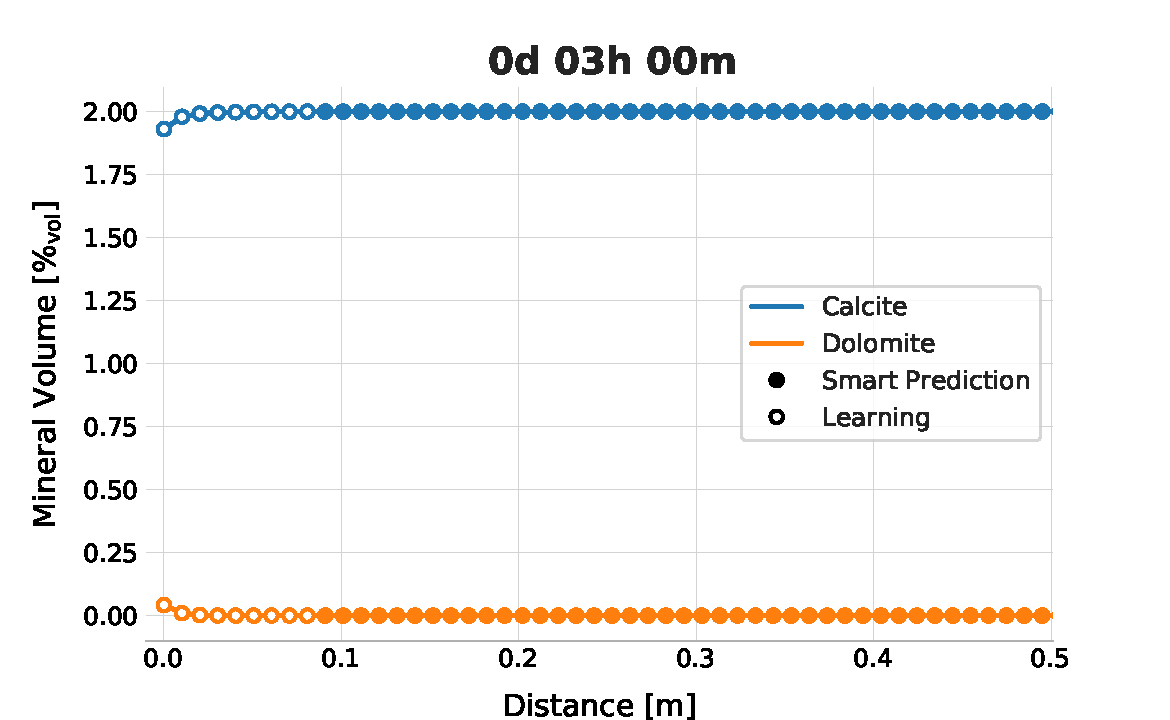
\includegraphics[width=0.46\textwidth, 
trim={0 0 1.5cm 0.5cm},clip]{figures/kinetics/calcite-dolomite-6}\label{fig:minerals-1}}}
\subfloat[]{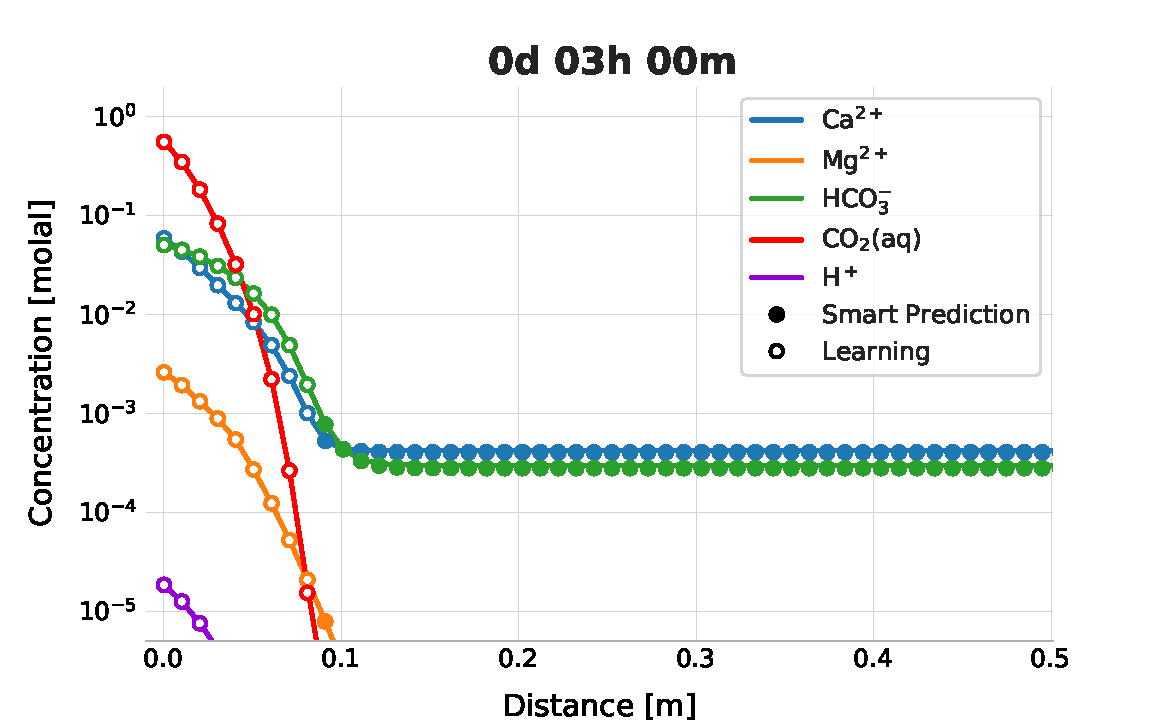
\includegraphics[width=0.46\textwidth, 
trim={0 0 1.5cm 0.5cm},clip]{figures/kinetics/aqueous-species-6}\label{fig:aqueous-1}} \\[-10pt]
%
\subfloat[]{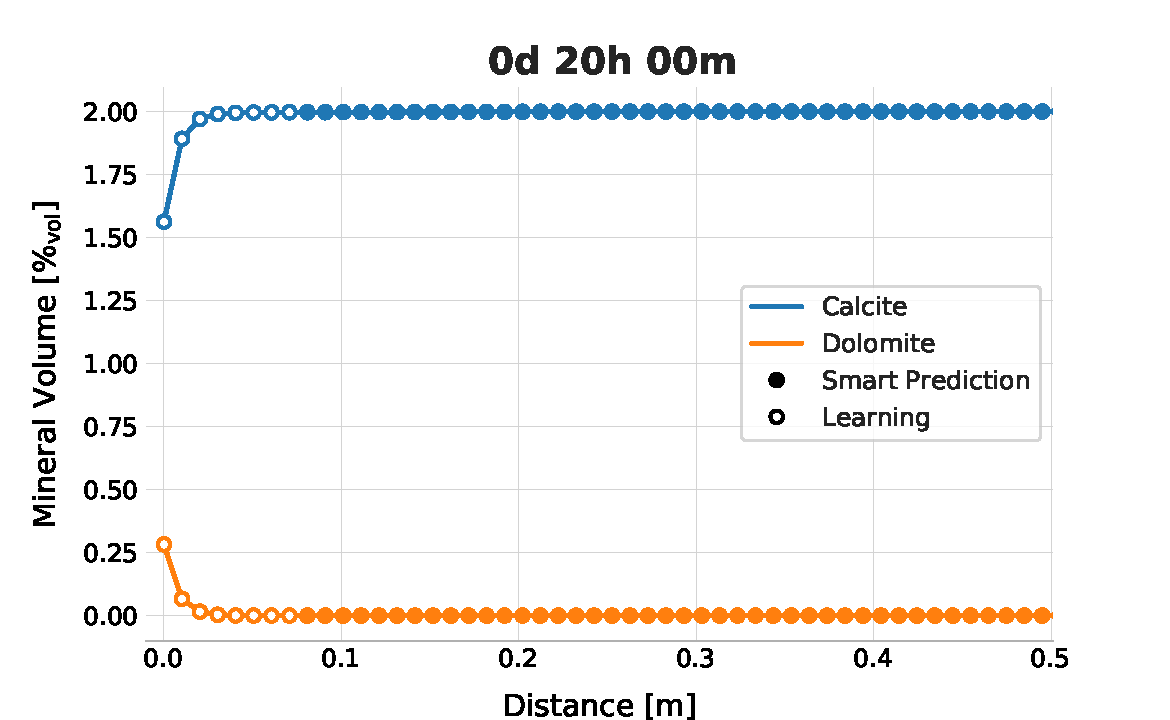
\includegraphics[width=0.46\textwidth, 
trim={0 0 1.5cm 0.5cm},clip]{figures/kinetics/calcite-dolomite-40}\label{fig:minerals-10}}
\subfloat[]{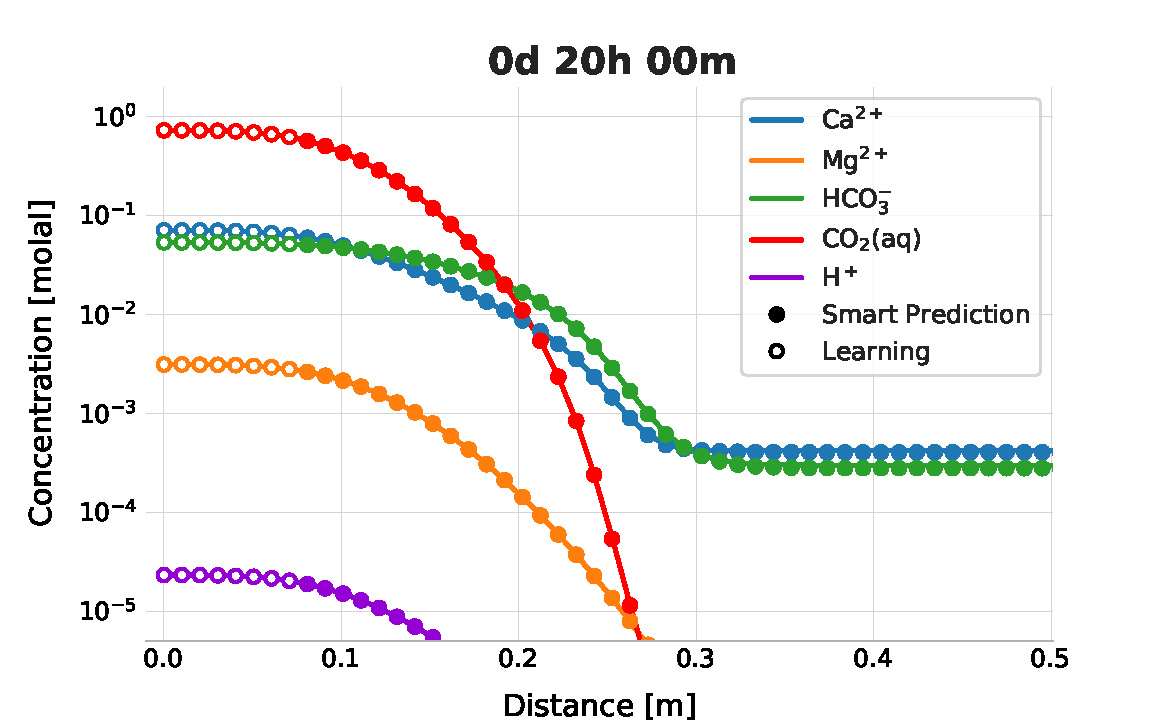
\includegraphics[width=0.46\textwidth, 
trim={0 0 1.5cm 0.5cm},clip]{figures/kinetics/aqueous-species-40}\label{fig:aqueous-10}}\\[-10pt]
%
\subfloat[]{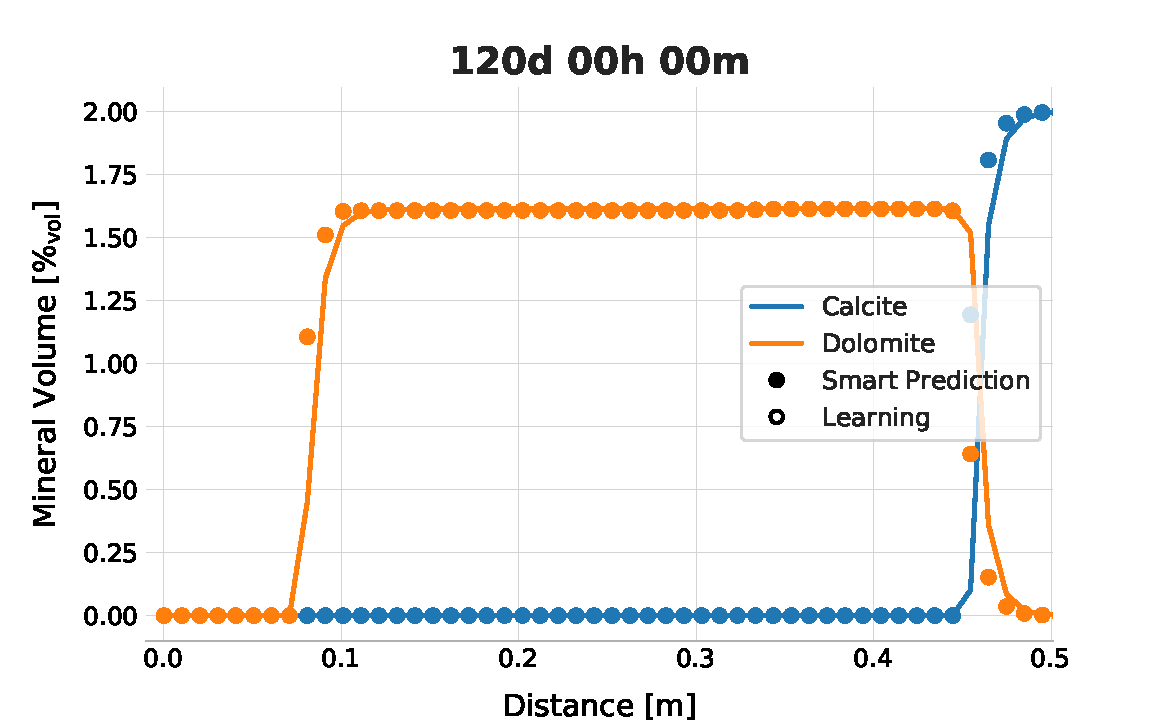
\includegraphics[width=0.46\textwidth, 
trim={0 0 1.5cm 0.5cm},clip]{figures/kinetics/calcite-dolomite-5760}\label{fig:minerals-5760}}
\subfloat[\sveta{TODO: replot}]{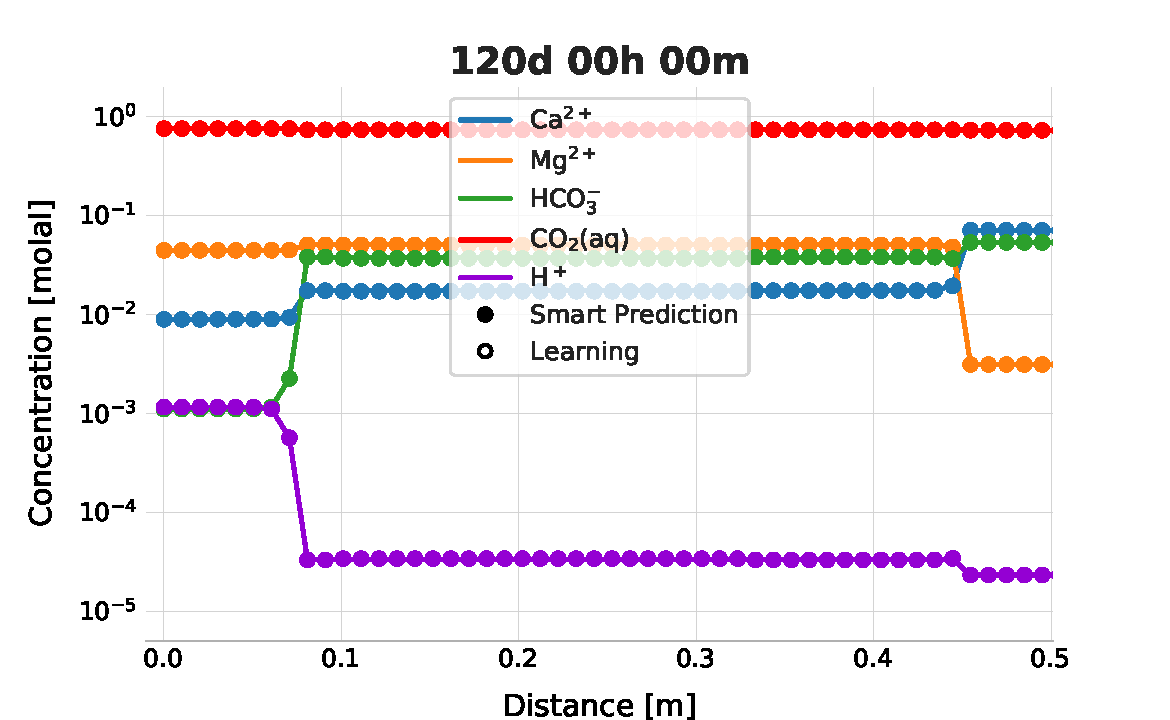
\includegraphics[width=0.46\textwidth, 
trim={0 0 1.5cm 0.5cm},clip]{figures/kinetics/aqueous-species-5760}\label{fig:aqueous-5760}}
\caption{
The volume percent ($\%_{{\rm vol}}$) of the minerals calcite and dolomite along the rock core as well 
as the concentrations of selected aqueous species (in molal) at three different times: 3 hours, 
20 hours, and 120 days (after 6, 40, and 5760 time steps of 30 minutes each, respectively). 
The \emph{solid curves} correspond to results of the reactive transport simulation using conventional
chemical kinetics calculations based on the integration of the system of ODEs for kinetically 
controlled species and update of the equilibrium species by the Gibbs energy minimization.
The circles ${\rm (}\bullet{\rm )}$ and ${\rm (}\circ{\rm )}$ correspond to the results using smart 
chemical kinetics calculations. \emph{Solid circles} ${\rm (}\bullet{\rm )}$ indicate successful
fast and accurate smart kinetics prediction at that point, whereas the \emph{empty circles} 
${\rm (}\circ{\rm )}$ depict the cells where \emph{on-demand learning/training} was needed.}
\label{fig:calcite-dolomite-kinetics}
\end{figure}

%---------------------------------------------------------------------------------------------------%

Figure~\ref{fig:calcite-dolomite-kinetics} shows the volume of minerals calcite and dolomite (left), 
as well as the concentrations of aqueous species (right) along the rock core at three different 
simulation times: 3 hours, 20 hours, and 120 days. As calcite dissolves, dolomite precipitates as 
the result of reaction releasing calcium ions with magnesium ions in the injected brine. 
After 3 hours of injecting the CO$_{2}$-saturated brine, a slight dissolution of calcite and 
precipitation of dolomite starts to take place. In Figures~\ref{fig:aqueous-1}, \ref{fig:aqueous-10}, 
and \ref{fig:aqueous-5760}, one can see an increase of the local concentrations of carbonic species 
CO$_{2}$(aq) and HCO$_{3}^{-}$(aq) because of the injected CO$_{2}$-saturated brine. 
The precipitated dolomite also gradually dissolves, as the injection of the acidic CO$_{2}$-saturated 
fluid continues. This can be seen in Figure~\ref{fig:minerals-5760} in the left region of the rock core, 
where neither calcite nor dolomite is present after 120 days of continuous brine injection. 
%
The concentrations of calcium ions increases as calcite and dolomite dissolves (see Figure 
\ref{fig:aqueous-5760}, between 0.0 and 0.1m or between 0.4 and 0.5m of rock). \sveta{TODO: re-plot 
the figure.} 

%---------------------------------------------------------------------------------------------------%
Figure~\ref{fig:calcite-dolomite-kinetics} confirms that the use of the smart chemical kinetics 
algorithm in combination with the smart equilibrium evaluation \emph{does not} compromise accuracy
during the simulation (except the slight delay in the mineral-phase changes in Figure 
\ref{fig:minerals-5760}). As agreed above, the solid circles ${\rm (}\bullet{\rm )}$ represent 
a successful (accurate enough) prediction of elements' amounts by the smart kinetic algorithm 
at that cell position and time step. The empty circles ${\rm (}\circ{\rm )}$ correspond to 
unsuccessful (not accurate enough) estimation, resulting in the full integration of the system 
Eq.\eqref{eq:kinetics}. 

%---------------------------------------------------------------------------------------------------%
Generally, the current implementation of the smart kinetics algorithm triggers more full evaluation 
of kinetic paths, which can be observed from Figure~\ref{fig:calcite-dolomite-kinetics} after 
3 hours or 20 hours of reactive transport simulations. The number of empty circles 
${\rm (}\circ{\rm )}$ reaches up to 10~cells out of total 100 at some time steps. 
%
However, the algorithm is still capable to accurately estimate the rest of the discretization points 
on the rock (see the solid circles $\bullet$). Analogous to results from Subsection 
\ref{subsec:part-1}, the majority of the learnings are needed as the perturbation 
front moves down the rock core. Having said that, eventually, the OMDL has learnt enough distinct 
chemical kinetic problems (most of them near the inlet face) which could be successfully used for 
quick and accurate estimates for the rest of the cells downstream. 

We note that even though the smart prediction can be not accurate enough in some cells for the kinetic 
species, the ODML can still successfully predict the remaining equilibrium species. This is reflected 
in the total numbers of the learnings needed for kinetics and equilibrium species. For the 
first ones, total 1808 (or 0.18\%) learnings of 1`000`000 cells are triggered after violating  
Eq.~\eqref{eq:acceptance-test-rates}. Update of the equilibrium species, in turn, required 
989 (0.10\%) full GEM simulations, allowing 99.90\% of the discretization cells to be predicted quickly.
%
For this particular example, we used $\epsilon_{\rm rel}=10^{-1}$ and $\epsilon_{\rm abs}=10^{-5}$ 
in Eq.~\eqref{eq:acceptance-test-rates} and the tolerances $\epsilon_{{\rm rel}}=10^{-1}$ and 
$\epsilon_{\rm abs}=10^{-12}$ for the acceptance criterion Eq.~\eqref{eq:acceptance-test-mu}.
%
Figure~\ref{fig:number-training-kinetics} presents the number of on-demand learning operations 
triggered during the reactive transport simulation by the ODML algorithm for either (a) kinetic or 
(b) equilibrium species. Much sparser distribution of trainings for the smart chemical equilibrium 
evaluation (i.e., Figure \ref{fig:number-training-kinetics-smart-equilibrium-2}) supports the numbers 
highlighted above, i.e., it needs about twice as less full GEM simulations in total. In both cases, 
most of the trainings occur during the first steps of reactive 
transport as a result of the incoming brine perturbing the fluid composition on the left side of 
the rock core. However, as time passes, only about 1 or 2 cells per time step need full evaluations 
occasionally. Eventually, the smart prediction algorithm becomes knowledgeable enough about the 
recurring equilibrium states in the simulation that it can quickly and accurately perform all 
subsequent equilibrium calculations without further learning, i.e., no trainings are triggered 
in the second half (after 5000 steps) of the reactive transport simulation (see Figure 
\ref{fig:number-training-kinetics-smart-equilibrium}. We plan to extend this example to the problem 
with more heterogeneous features (e.g., the one presented in Subsection \ref{subsec:part-3}), 
to investigate how it might influence the rate of on-demand learning operations both 
in kinetics and equilibrium.

%---------------------------------------------------------------------------------------------------%
\begin{figure}[!t]
\begin{centering}
\subfloat[Number of on-demand learnings for kinetic species]{
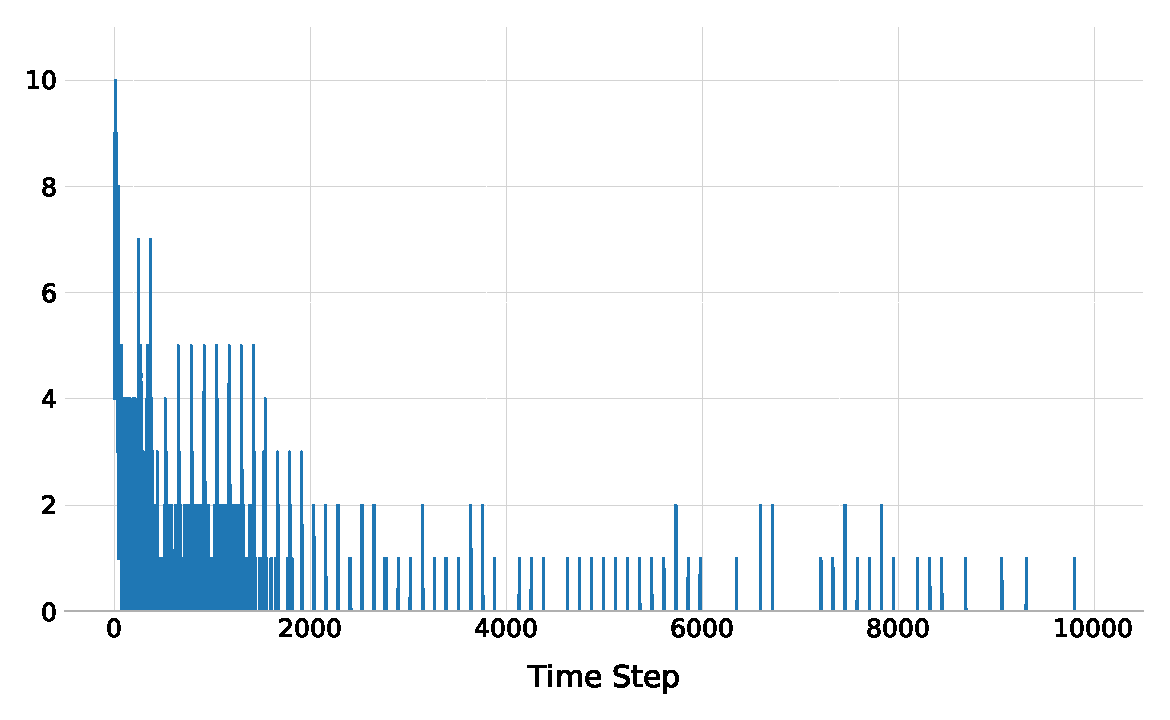
\includegraphics[width=0.6\textwidth, 
trim={0.0cm 1cm 0.5cm 0cm}, clip]{figures/kinetics/on-demand-learning-countings}} \\[-2pt]
\subfloat[Number of on-demand learnings for equilibrium species]{
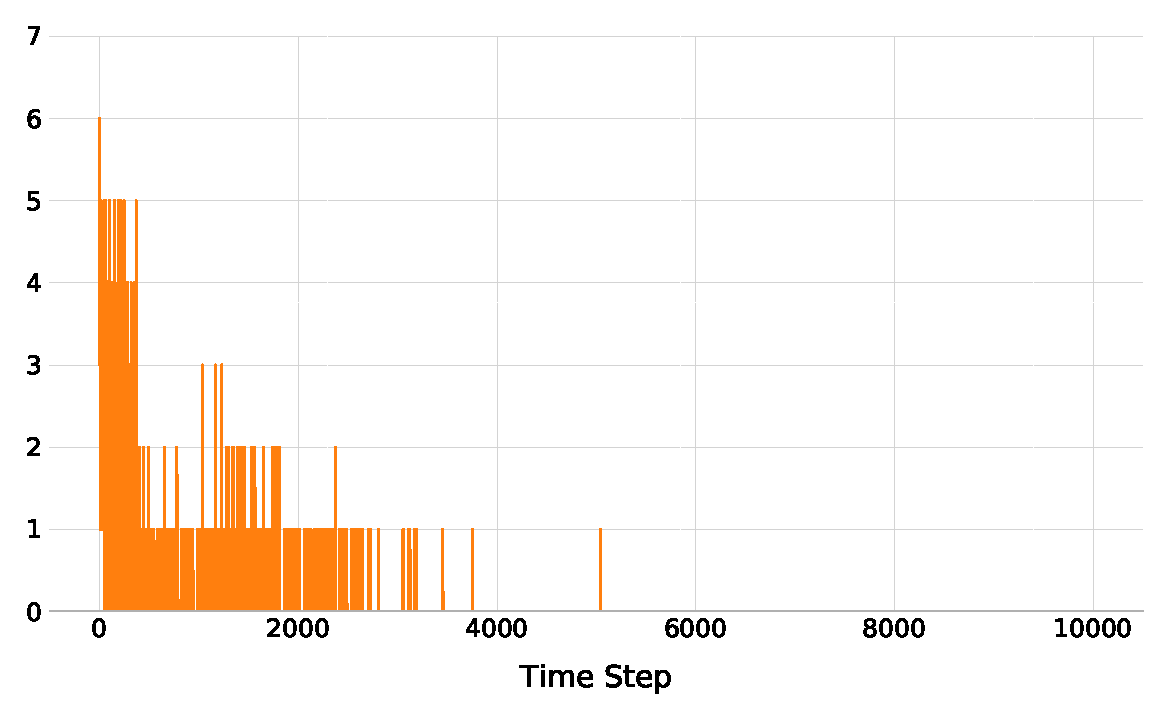
\includegraphics[width=0.6\textwidth, 
trim={0.0cm 1cm 0.5cm 0cm}, clip]{figures/kinetics/on-demand-learning-countings-equilibrium}
\label{fig:number-training-kinetics-smart-equilibrium-2}
\label{fig:number-training-kinetics-smart-equilibrium}}
\par\end{centering}
\caption{\label{fig:number-training-kinetics}
\emph{On-demand learning} operations triggered by the (a) smart chemical kinetics and (b) smart 
chemical equilibrium algorithm during the reactive transport simulation using a mesh with 100 cells.
The test has performed 10'000 time steps yielding 1'000'000 chemical kinetics and equilibrium 
problems. 
%
(a) Only 1808 (or 0.18\%) of these were solved using the full numerical integration of the system of 
ODEs for kinetically controlled species, the rest 99.82\% were quickly and accurately estimated 
ODML algorithm.
(b) For the update of equilibrium species, 989 problems (0.10\%) required full GEM simulations, 
allowing 99.90\% of the discretization cells to be predicted quickly.}
\end{figure}

%---------------------------------------------------------------------------------------------------%
\begin{figure}[!t]
\begin{centering}
\subfloat[The ODML applied for kinetics only]{
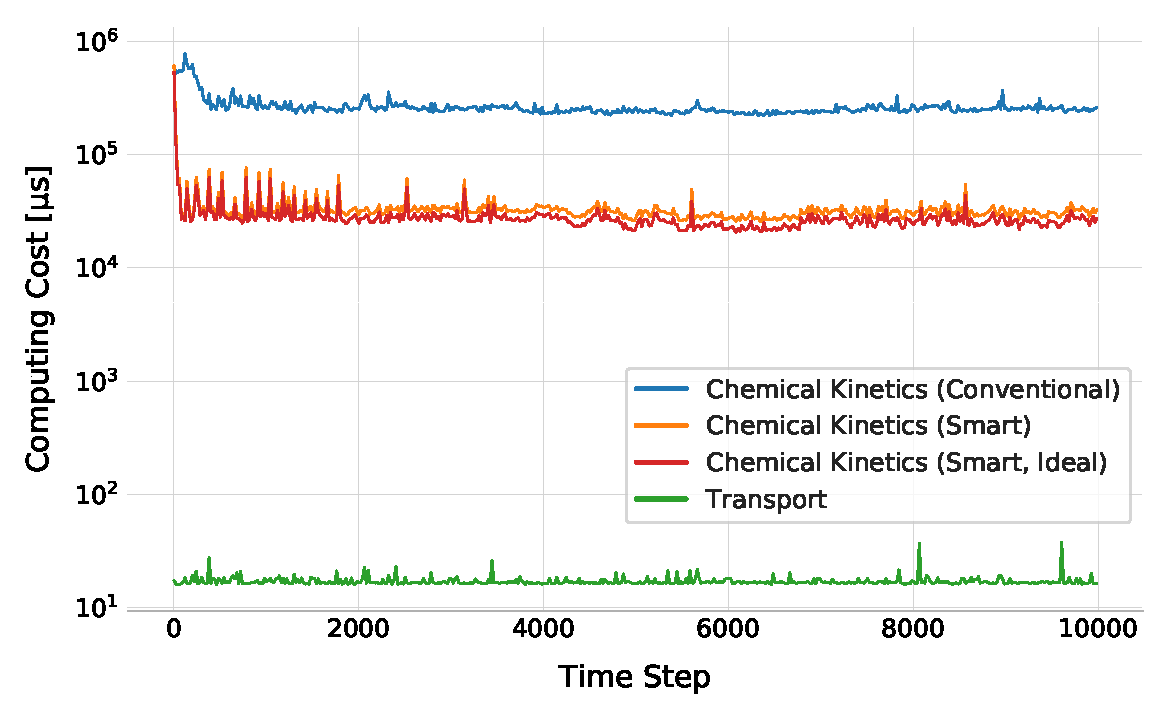
\includegraphics[width=0.6\textwidth]{figures/kinetics-only/computing-costs} \label{fig:computational-cost-kinetics-1}} \\[-2pt]
\subfloat[The ODML applied for both kinetics and equilibrium]{
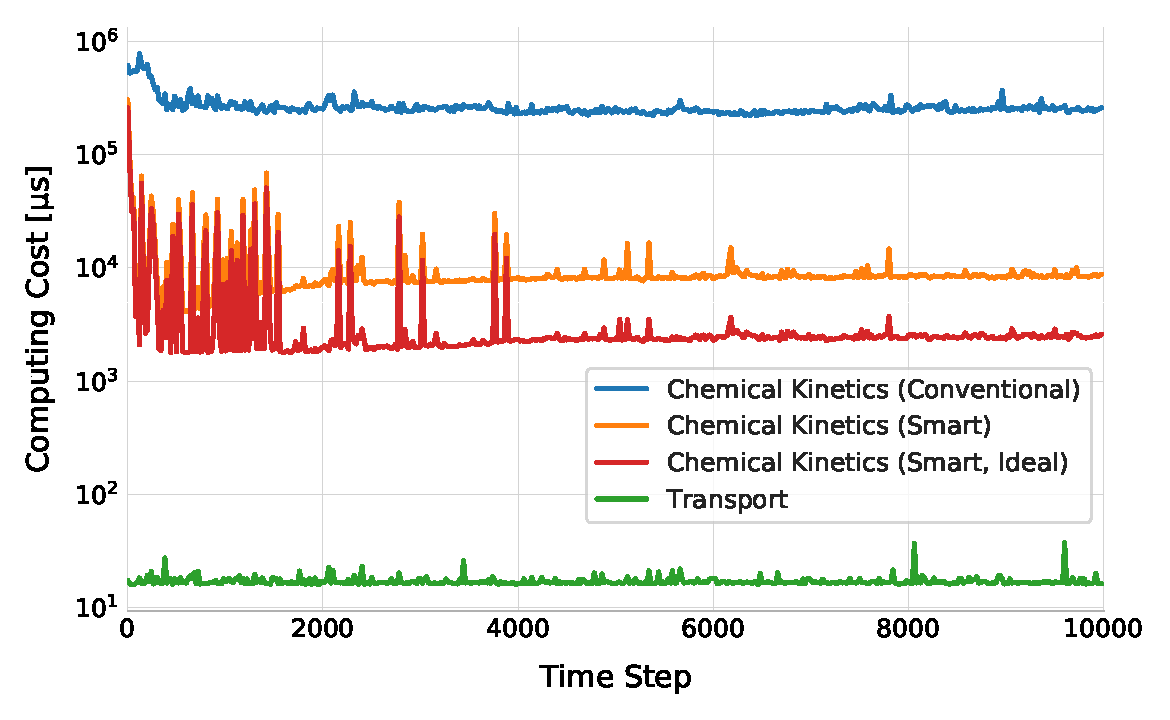
\includegraphics[width=0.6\textwidth]{figures/kinetics/computing-costs}
\label{fig:computational-cost-kinetics-2}}
\par\end{centering}
\caption{\label{fig:computational-cost-kinetics}
Comparison of the computing costs (CPU time in microseconds) of transport, conventional, smart 
chemical kinetics calculations, and \emph{zero-search-cost} smart kinetics calculations per each 
RT time step, where (a) ODML applied for kinetics only and (b) ODML applied for both kinetics and 
equilibrium. The cost of kinetics calculations per time step is the sum of the costs of kinetic 
and equilibrium species' amount recovery in each mesh cell. The transport costs correspond to the 
time needed for solving the discretized algebraic transport equations. The zero-search-cost smart 
kinetics calculation excludes the cost of reference elements look-up both for kinetic and equilibrium 
species smart estimation.}
\end{figure}
%---------------------------------------------------------------------------------------------------%
Similarly to the previous subsection, Figure~\ref{fig:computational-cost-kinetics} compares the 
computational cost at each time step of: 
\emph{(i)} conventional chemical kinetics calculations, 
\emph{(ii)} smart chemical kinetics 
\emph{(iii)} zero-cost-search smart algorithm calculations, and \emph{(iii)} transport calculations. 
Here, two implementations are compared: application of the ODML strategy to only kinetics 
(see Figure \ref{fig:computational-cost-kinetics-1}) and the use of the smart approach for both 
kinetics and equilibrium computations (see Figure \ref{fig:computational-cost-kinetics-2}).
%
For the chemical kinetics calculations, whether it is conventional or smart, we show CPU time 
(in microseconds) needed to calculate all kinetic and equilibrium states across all mesh cells within 
the same time step. The cost of transport calculations corresponds to the time needed to solve the 
algebraic transport equations. The zero-cost-search smart kinetics calculations are the costs of 
ODLM per each reactive transport step excluding the costs for retrieval of reference state to perform 
Taylor expansions using Eq.\eqref{eq:smart-estimate} and Eq.\eqref{eq:smart-estimate-kinetics} for 
kinetic and equilibrium species, respectively.

%---------------------------------------------------------------------------------------------------%
We see that combination of smart approach for both kinetics and equilibrium (illustrated 
in Figure \ref{fig:computational-cost-kinetics-2}) considerably improves the computational costs of 
chemical calculations (by about half of order of magnitude) in comparison to Figure \ref{fig:computational-cost-kinetics-1}.
%---------------------------------------------------------------------------------------------------%
Overall, the application of the ODML algorithm for kinetics and equilibrium species reduces the cost 
of conventional approach by one and a half orders of magnitude (see 
Figure~\ref{fig:computational-cost-kinetics-2}). At the same time, since chemical kinetics is way 
more complex chemical process, it requires higher computational costs in comparison to pure 
equilibrium presented in Figure \ref{fig:computational-cost}. We also note that during 
the first time steps of reactive transport simulation, the CPU time spent on the smart kinetic 
algorithm has much higher spikes. They correspond to the learnings happening for both kinetics and 
equilibrium species. After about half of the simulation time, 
they are much smaller and more seldom. The red line, corresponding to the zero-cost-search 
smart kinetics calculations, depicts the potential improvement in the CPU time of the ODML algorithm 
(up to two orders of magnitude improvement of the conventional time) once the costs of the reference 
point retrieval are minimized. 
%

To illustrate again how much the lookup time influences the total time of the estimation step in the
ODML algorithm, we use Figure~\ref{fig:search-traylor-vs-total-learnings-kinetics}. It is depicted 
together with the costs of performing a first-order Taylor expansion (which corresponds to considerably 
fast matrix-vector multiplication). Unlike in Figure~\ref{fig:search-traylor-vs-total-learnings}, 
where lines were relatively close to each other, NN search (blue line) is almost an order of 
magnitude more expensive than the time needed to construct the smart prediction. This is due to a larger 
amount of the saved reference chemical states for chemical kinetics (1808) and equilibrium (989) 
verses 258 in the example considered in Subsection \ref{subsec:part-1}. 
%
\begin{figure}[!t]
\begin{centering}
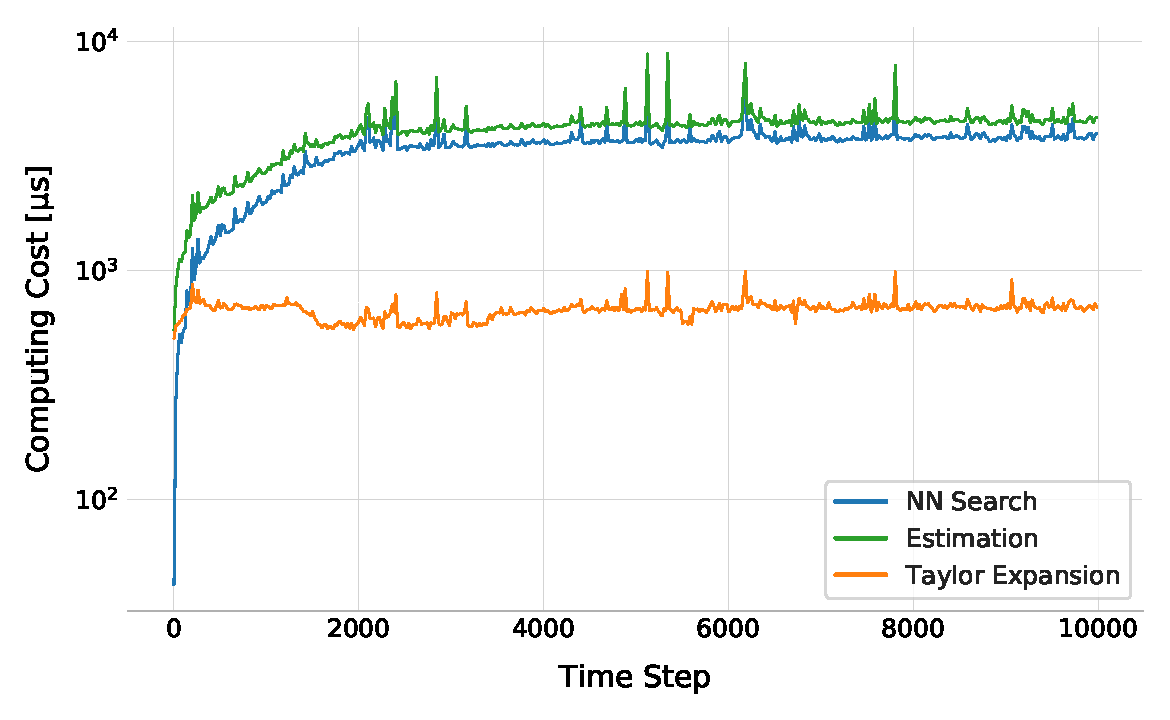
\includegraphics[width=0.6\textwidth]{figures/kinetics/estimate-search-costs.pdf}
\par\end{centering}
\caption{\label{fig:search-traylor-vs-total-learnings-kinetics}
%
The speedup factor of chemical equilibrium calculations, at each time step of the simulation, 
resulting from the use of the on-demand learning acceleration strategy, employing a linear NN search 
(orange). A comparison is made with the speedup obtained by removing the computing time needed for 
the retrieval of the reference state (blue). The latter indicates an upper bound for the speedup 
upon improvement of the search algorithm.}
\end{figure}

%---------------------------------------------------------------------------------------------------%
To analyse the speedup obtained with the current implementation, we consider Figure \ref{fig:speedup-with-and-without-search-costs-kinetics}. Again, two versions of the 
smart kinetics algorithm are considered: Figure \ref{fig:speedup-with-and-without-search-costs-kinetics-1}
corresponds to the case where the ODML is applied to chemical kinetics only, and in Figure
\ref{fig:speedup-with-and-without-search-costs-kinetics-2} the smart approach accelerates both kinetics
and equilibrium. We note that the combined approach (8-10x faster) provides several times higher 
acceleration than the one for kinetics only (30-100x). In the second part of the reactive transport 
simulations (see Figure~\ref{fig:speedup-with-and-without-search-costs-kinetics-2}) it stabilizes 
its average value 30. 
%
If we ignore the costs of the retrieval operation discussed above, it yields the approximate upper 
bound of the speedup, which can be obtained (orange line). The average value of this potential 
speed-up is around 100. 
%
%---------------------------------------------------------------------------------------------------%
\begin{figure}[!t]
\begin{centering}
\subfloat[The ODML applied for kinetics only]{
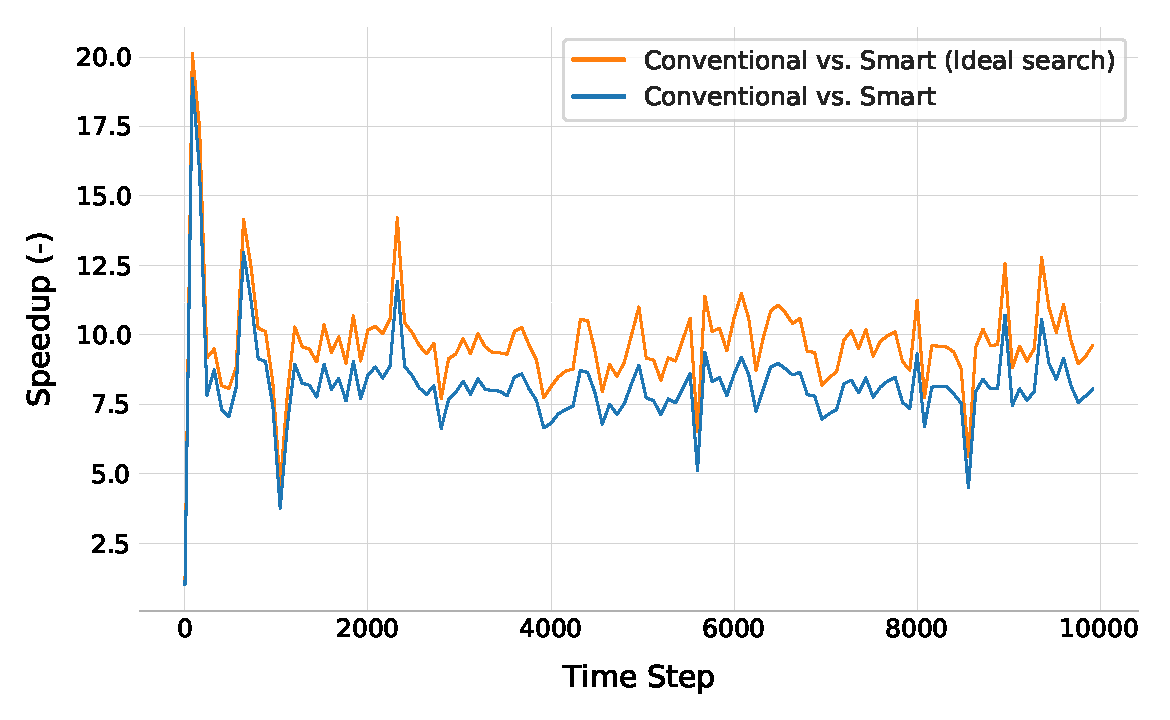
\includegraphics[width=0.66\textwidth]{figures/kinetics-only/speedups}
\label{fig:speedup-with-and-without-search-costs-kinetics-1}} \\[-2pt]
\subfloat[The ODML applied for both kinetics and equilibrium]{
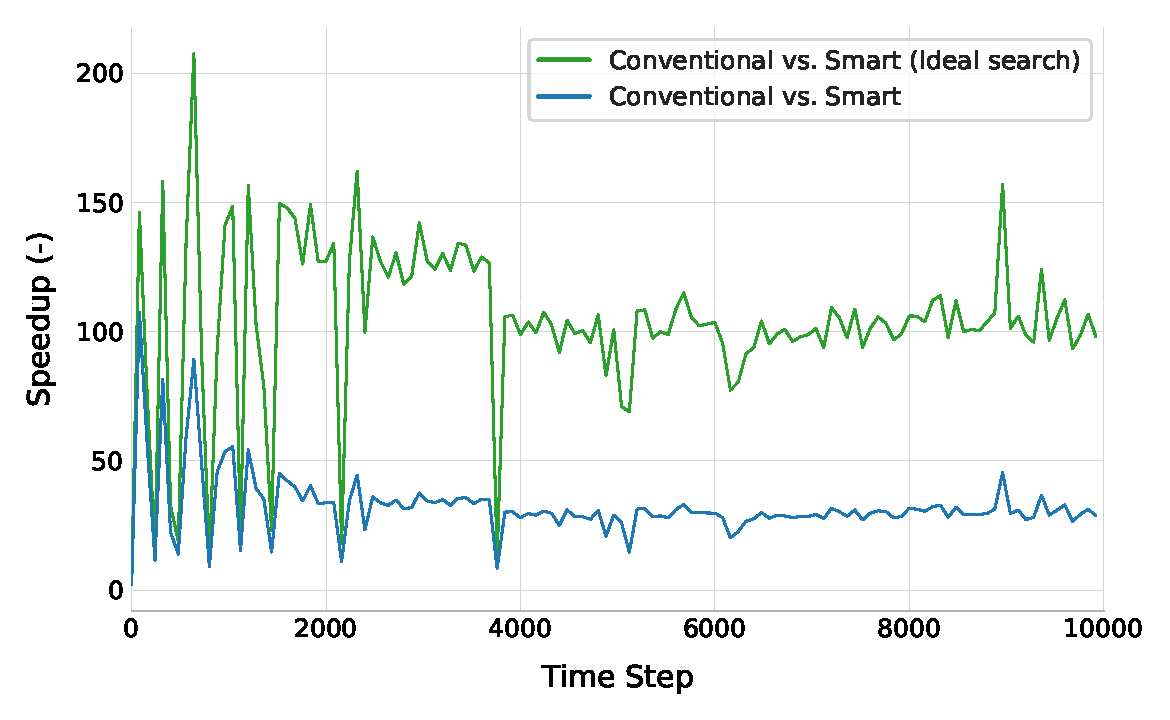
\includegraphics[width=0.6\textwidth]{figures/kinetics/speedups}
\label{fig:speedup-with-and-without-search-costs-kinetics-2}}
\par\end{centering}
\caption{\label{fig:speedup-with-and-without-search-costs-kinetics}
The speedup factor of chemical kinetics calculations, at each time step of the simulation, 
resulting from the use of the on-demand learning acceleration strategy, employing a linear NN search 
(blue), where (a) ODML applied for kinetics only and (b) ODML applied for both kinetics and 
equilibrium. A comparison is made with the speedup obtained by removing the computing time needed for 
the retrieval of the reference state (green). The latter indicates an upper bound for the speedup 
upon improvement of the search algorithm.}
\end{figure}

%---------------------------------------------------------------------------------------------------%
\begin{figure}[!t]
\begin{centering}
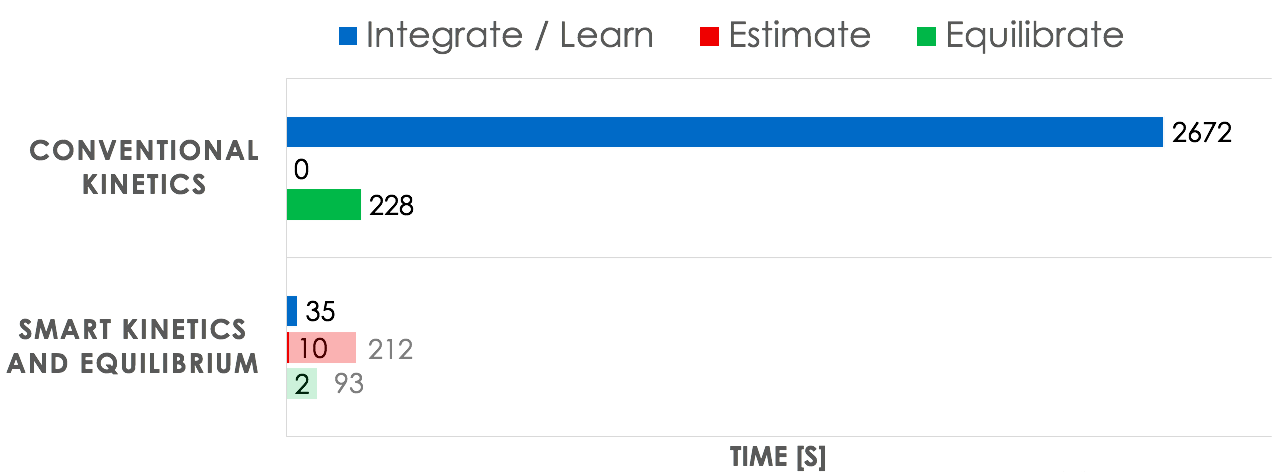
\includegraphics[width=0.8\textwidth]{figures/kinetics/diagram-times}
\par\end{centering}
\caption{\label{fig:diagram}
Comparison of the time spent for the different simulation steps, `Integrate/Learn', `Estimate', and 
`Equilibrate' using either conventional kinetics approach or smart kinetics approach combined with 
smart equilibrium. .}
\end{figure}
%
To better explain the distribution of time spent for different stages of the considered approaches, 
we consider a particular run of this numerical test with conventional algorithm first. Then, the time
spend for this simulation is divided to the integration of the kinetic species and the subsequent 
equilibration of the rest of them. The upper part of the diagram in Figure \ref{fig:diagram} shows
that `Integrate /Learn' step required 2672~s (44.53~minutes) and `Equilibrate' step needs 228~s 
(3.8~minutes).
%
If the same test is performed with the ODML algorithm (see the lower part of the diagram with the 
name Smart Kinetics and Equilibrium), the time for the `Integrate/Learn' step is reduced to 35s (approx. 
half a minute) and `Equilibrate' one is to 93s or 1.5 minutes (see light green bar). However, 
in this smart approach, we introduce a new step `Estimate' that still takes majority of time, i.e., 
212~s or 3.5 minute (see pink bar). Both `Estimate' steps `Equilibrate' still includes the costs of 
the search (currently being a bottleneck to demonstrate the algorithm's performance). Their removal 
can minimise the cost down to 10~s and 2~s (red and green bars), respectively. That is why this issue 
will be prioritized in the next steps of our investigation. 

%---------------------------------------------------------------------------------------------------%
{\bf Note}: Application of the ODML method to the systems with more than one kinetically controlled 
reactions indicates a potential for even higher speedups, i.e., {\bf 35-102x} for 2 reactions and 
{\bf 92-124x} for 3 reactions. This is rather expected due to the replacement of even more complex 
systems of ODEs by a simple yet accurate Taylor expansion.

\subsection{Coupling of Reaktoro with Firedrake on two-dimensional reactive transport problem 
\label{subsec:part-3}}

For the purpose of modelling more challenging high-dimensional heterogeneous reactive transport 
problem, Reaktoro was coupled with \texttt{Firedrake} \cite{Rathgeber2016}, an open-source software 
for solving partial differential equations (PDEs) with finite element method (FEM). It is automated 
system that provides expressive specification of any PDE (advection, diffusion, Darcy equation, etc.) 
using the Unified Form Language from the FEniCS Project \cite{LoggMardalEtAl2012a, AlnaesBlechta2015a}. 
We envision a new project called \texttt{Rok} for further development of reactive transport simulator 
powered by Reaktoro and Firedrake. 
%---------------------------------------------------------------------------------------------------%

For reactive transport model, we consider similar problem to the one described in Section 
\ref{subsec:part-1} but for two-dimensional rock of the size $L_x \times L_y$ = 
$1.6 {\rm m} \times 1.0 {\rm m}$. The spacial mesh discretizing the rock contains $10 \time 10$ 
quadrilateral elements, resulting in $121$ degrees of freedom (DOFs). The reactive transport runs 
for $**$ steps with the time step defined by the CLF number, we fix to be 0.3, i.e., 
%
$$\Delta t = {\rm CFL} / \max \Big\{ \max |u_x| / h_x, \max |u_y| / h_y \Big\},$$ 
%
where $\boldsymbol{u} = [u_x; u_y]^{\rm T}$, and $h_x$ and $h_y$ define sizes of 
discretisation mesh along $x$ and $y$ coordinates, respectively. 

For the variable-density single-flow Darcy's equation
%
\begin{equation}
\begin{array}{rl}
\nabla (\varrho \boldsymbol{u}) &\: = \:f, \\
                 \boldsymbol{u} &\: = \:- \tfrac{k}{\mu} \nabla p,
\end{array}
\label{eq:darcy}
\end{equation}
%
the Darcy and the pore velocity $\boldsymbol{v}$ and $\boldsymbol{u}$, respectively, are related by
the rock porosity $\phi$, i.e., $\boldsymbol{u} = \tfrac{\boldsymbol{v}}{\phi}$. 
%---------------------------------------------------------------------------------------------------%
Here, we consider zero source-term $f = 0$, the water density $\varrho = 1000.0$ (kg/m3), and 
the water viscosity $\mu = 8.9 \cdot 10^{-4}$. The heterogeneous permeability $k$ of the rock with 
preferential flow path (see Figure \ref{fig:rok-permiability}) is provided by the open-source tool \texttt{\href{https://github.com/GeoStat-Framework/GSTools}{GeoStatTools}} \citep{GSTools2019} for 
the random field generation.
%
\begin{figure}[!t]
	\centering
	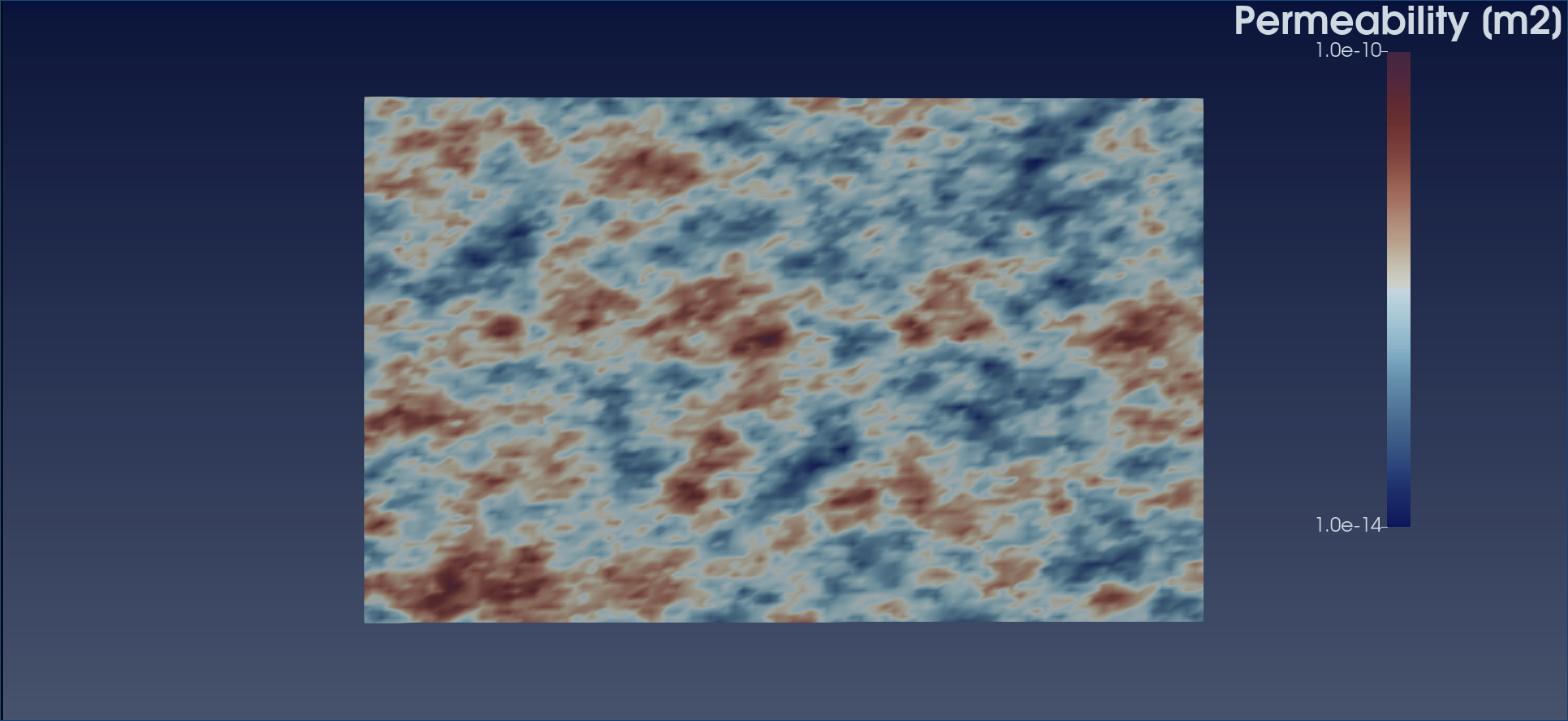
\includegraphics[width=0.7\textwidth, trim= 0 2cm 0 0, clip]{figures/rok/permiability.png}
	\caption{\label{fig:rok-permiability}
	Heterogeneous permeability field with preferential flow path (generated by the GSTools).}
\end{figure}
%
To solve the Darcy’s system for the velocity and pressure variables the Stabilized Dual Hybrid Mixed 
(SDHM) method is considered. The pressure field is reconstructed by the continues Galerkin elements 
of the first order (or ${\rm P}1$), whereas the flux is recovered by piece-wise constant elements 
P0. For the boundary condition (BC) of Darcy's flow problem \ref{eq:darcy}, we 
consider Dirichlet BC for the pressure on the left and right boundary, i.e., $p_{\rm L} = 10100$~Pa 
and $p_{\rm R} = 10^5$ Pa. Whereas, for the velocity, the zero Neumann condition on the top and 
the bottom of the rock is assigned, i.e., $v|_T \cdot n = v|_B \cdot n = 0$.

Using first-order operator splitting (see Appendix \ref{sec:Reactive-Transport-Equations}), 
we alternate between solving the transport and reaction equation. In the transport problem 
(reformulated for the concentrations of each element in fluid and solid partitions 
$\partial b_{j}^{\rm f}$ and $\partial b_{j}^{\rm s}$, $j = 1, \ldots, E$), 
%
\begin{equation}
\frac{\partial b_{j}^{\rm s}}{\partial t} 
+ \frac{\partial b_{j}^{\rm f}}{\partial t} 
+ \nabla\cdot(\boldsymbol{v}b_{j}^{\rm f} - D\nabla b_{j}^{\rm f})= q_i,
\label{eq:transport}
\end{equation}
%
the diffusion coefficient $D$ is assumed to be $10^{-9}~{\rm m}^2/{\rm s}$. Here, the pore velocity 
$\boldsymbol{v}$ and pressure $p$ follow from the numerical solution of flow problem 
Eq.~\ref{eq:darcy} (see Figure \ref{fig:darcy-velocity}). 
%
\begin{figure}[!t]
\centering
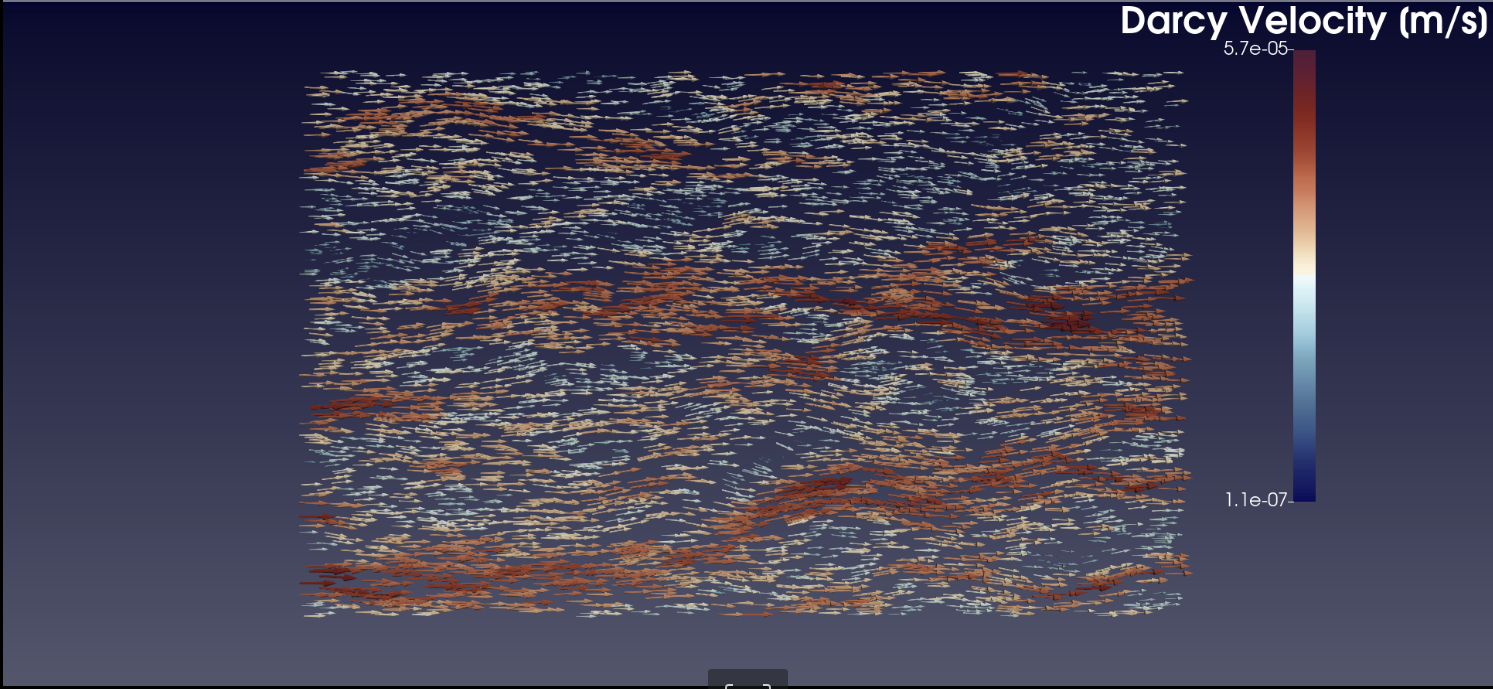
\includegraphics[width=0.7\textwidth, trim= 0 1cm 0 0, clip]{figures/rok/darcy-velocity.png}
\caption{The approximate Darcy velocity reconstructed solving Eq.\ref{eq:darcy} for $p$ and 
$\boldsymbol{u}$.}
\label{fig:darcy-velocity}
\end{figure}

%---------------------------------------------------------------------------------------------------%
After $\partial b_{j} = \partial b_{j}^{\rm s} + \partial b_{j}^{\rm s}$ is is transported 
by Eq.~\ref{eq:transport}, the chemical equilibrium calculations are performed in each cell/DOF. 
For the transport solver we apply Streamline-Upwind Petrov–Galerkin (SUPG) Method. To obtain 
chemical equilibrium speciation, we use Gibbs energy minimization (GEM) approach. 


The brine, injected on the left face of the rock, is a mixture of 1~kg of water with 0.90~moles of 
NaCl, 0.05~moles of MgCl$_{2}$, 0.01~moles of CaCl$_{2}$, 0.75~moles of CO$_{2}$, and 1.0~umoles of 
O$_{2}$.
%
Figure \ref{fig:rok-minerals} demonstrates the mineral composition of the porous rock at different 
moment in time as the result of reactive transport of continuous acidic aqueous fluid is injected 
on the left boundary. The simulation starts from the 10\% porous rock containing 2\% of Calcite 
(blue) in Figure \ref{fig:rok-minerals}(a). Figure \ref{fig:rok-minerals}(b) illustrates the first 
phase change from dissolving Calcite to precipitating Dolomite. However, as brine is being 
continuously injected, Dolomite gets eventually dissolved (see remaining Quartz in  grey). 
Figures \ref{fig:rok-minerals}(c)--(d) demonstrate how the transport continues in time. The 
fingering behaviour of Calcite 
(e.g., the finger in the middle of the rock) corresponds to provided by the permeability preferential path. 
The change in the aqueous species is illustrate in Figure \ref{fig:rok-aqueous-species}. 
We see the increase in 
Ca$^{2+}$, Mg$^{2+}$, and HCO$_3^{-}$ ion concentrations, as well as CO$_2$(aq) as brine is being injected.
%
\begin{figure}[!t]
\begin{centering}
\subfloat[]{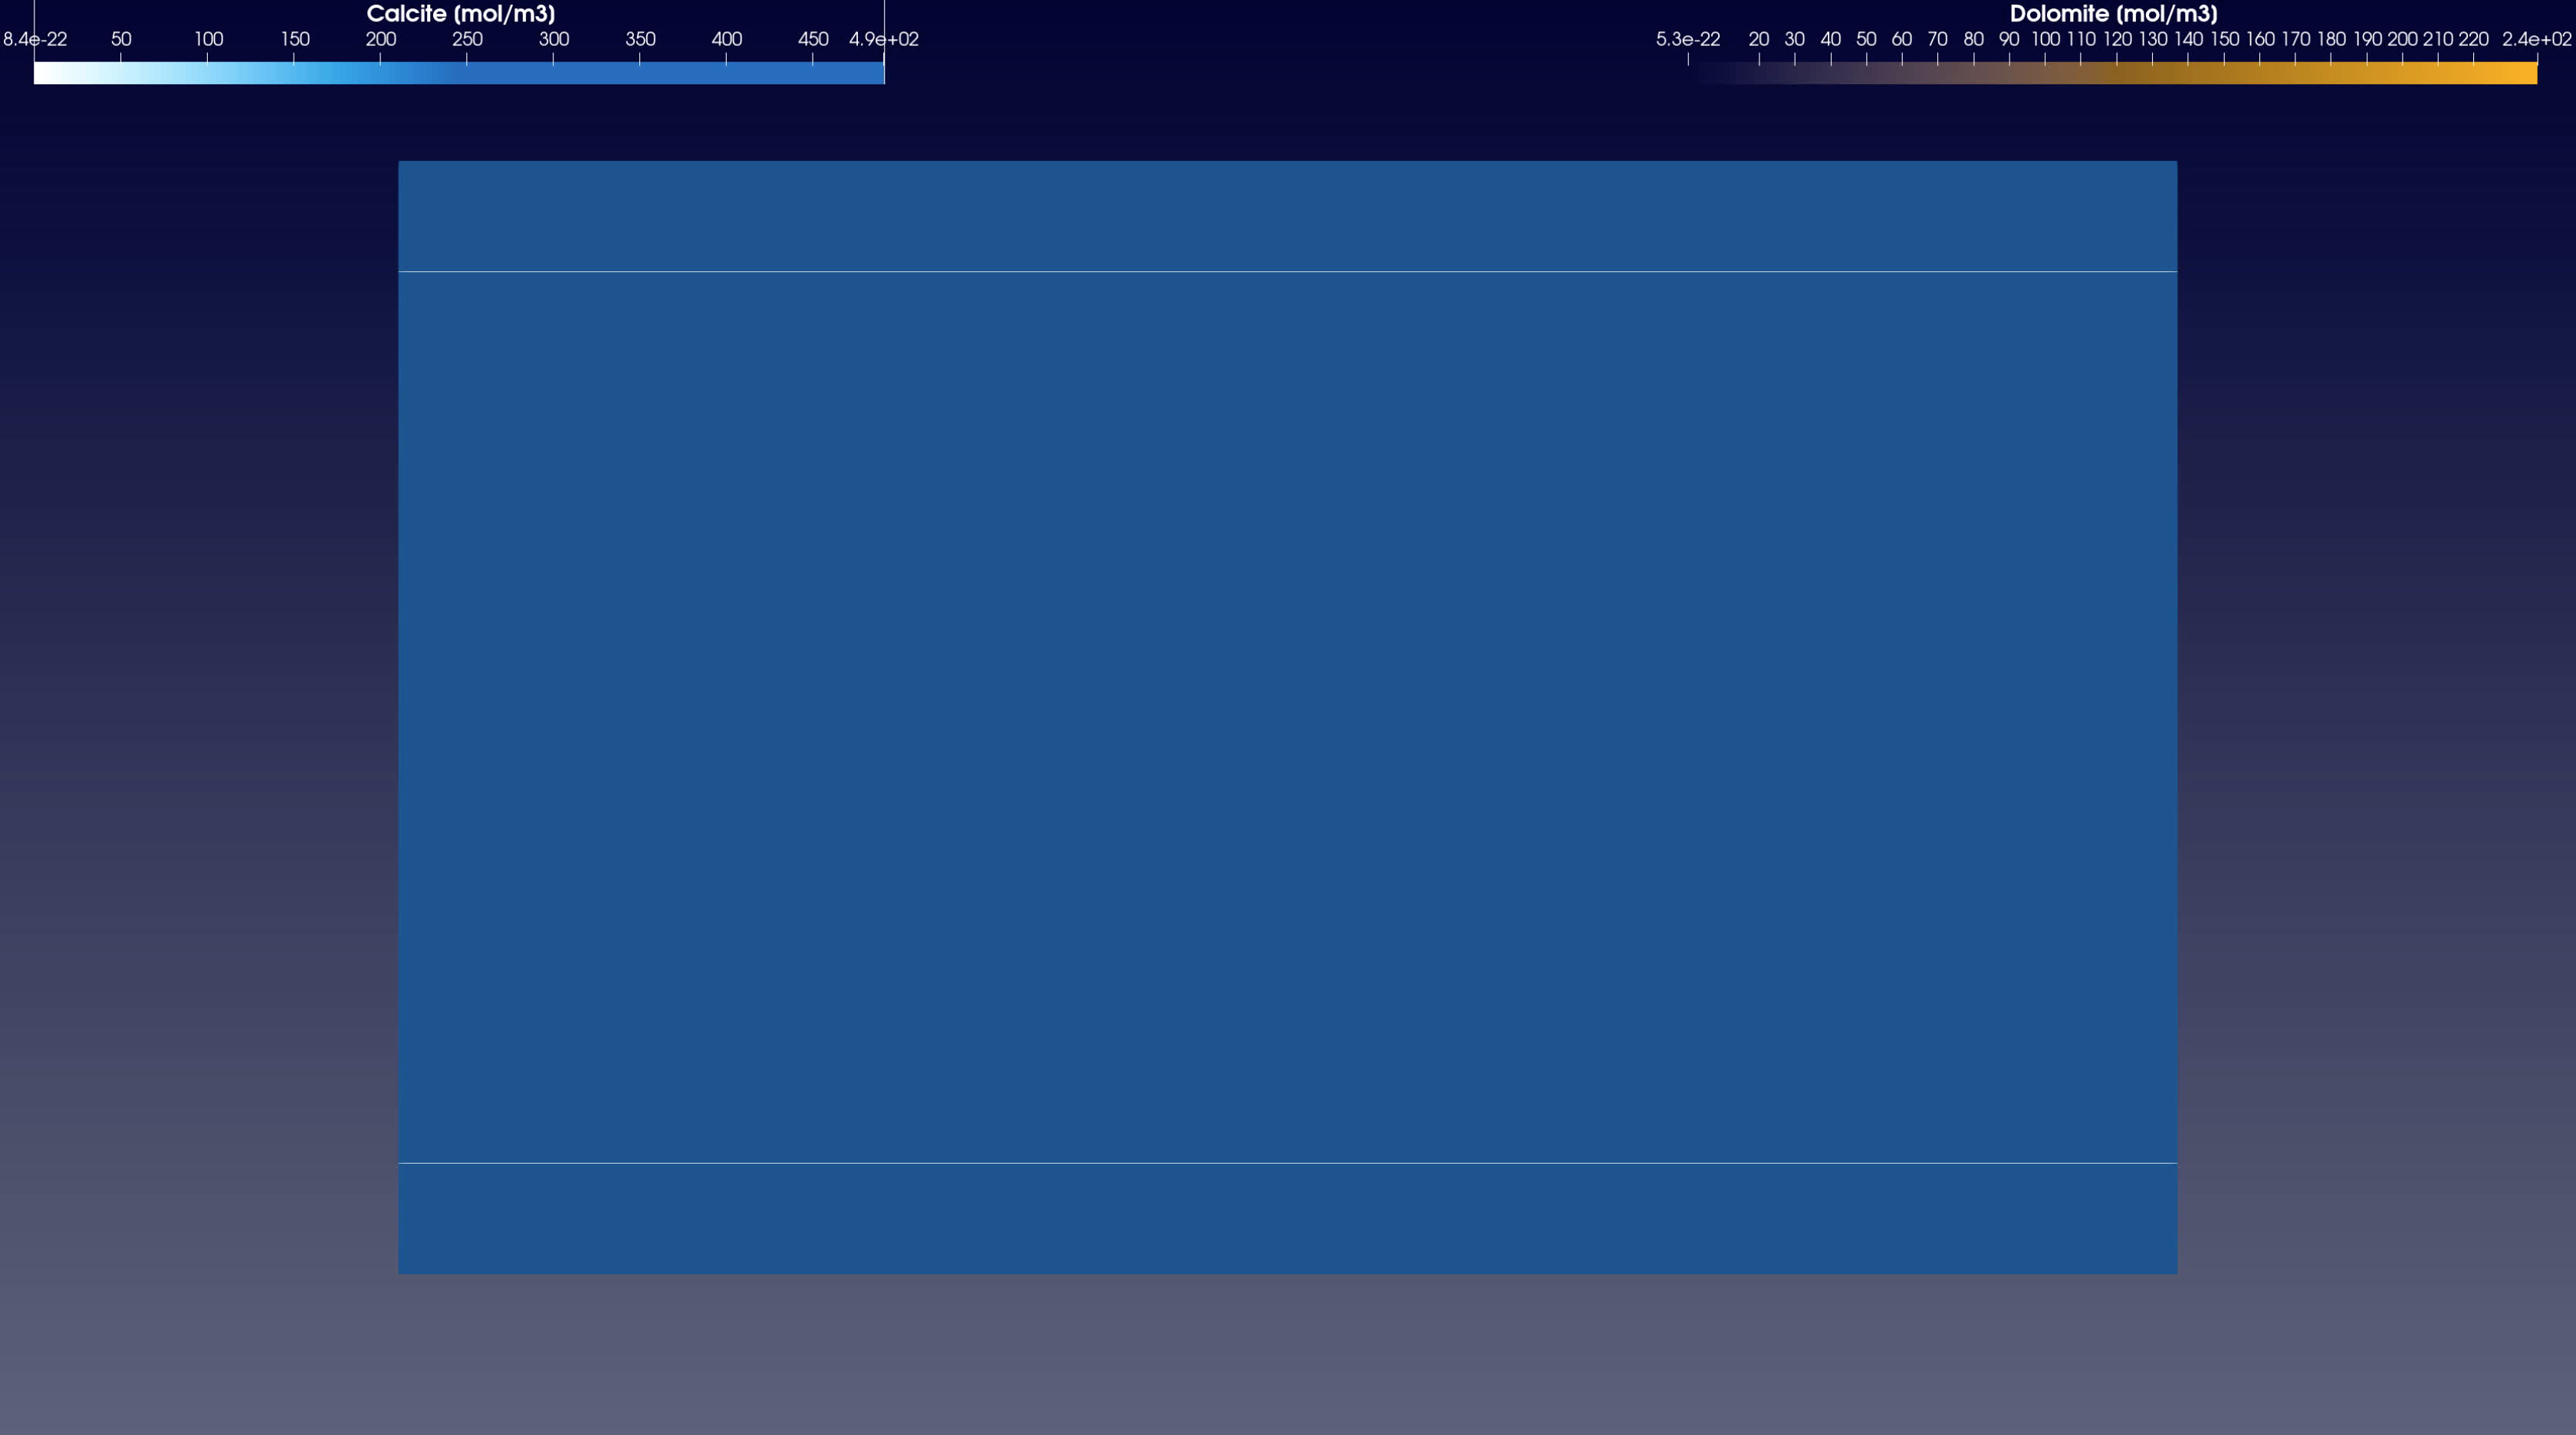
\includegraphics[width=0.45\textwidth, trim= 0 3cm 0 0, clip]{figures/rok/minerals-0s.png}}\quad
\subfloat[]{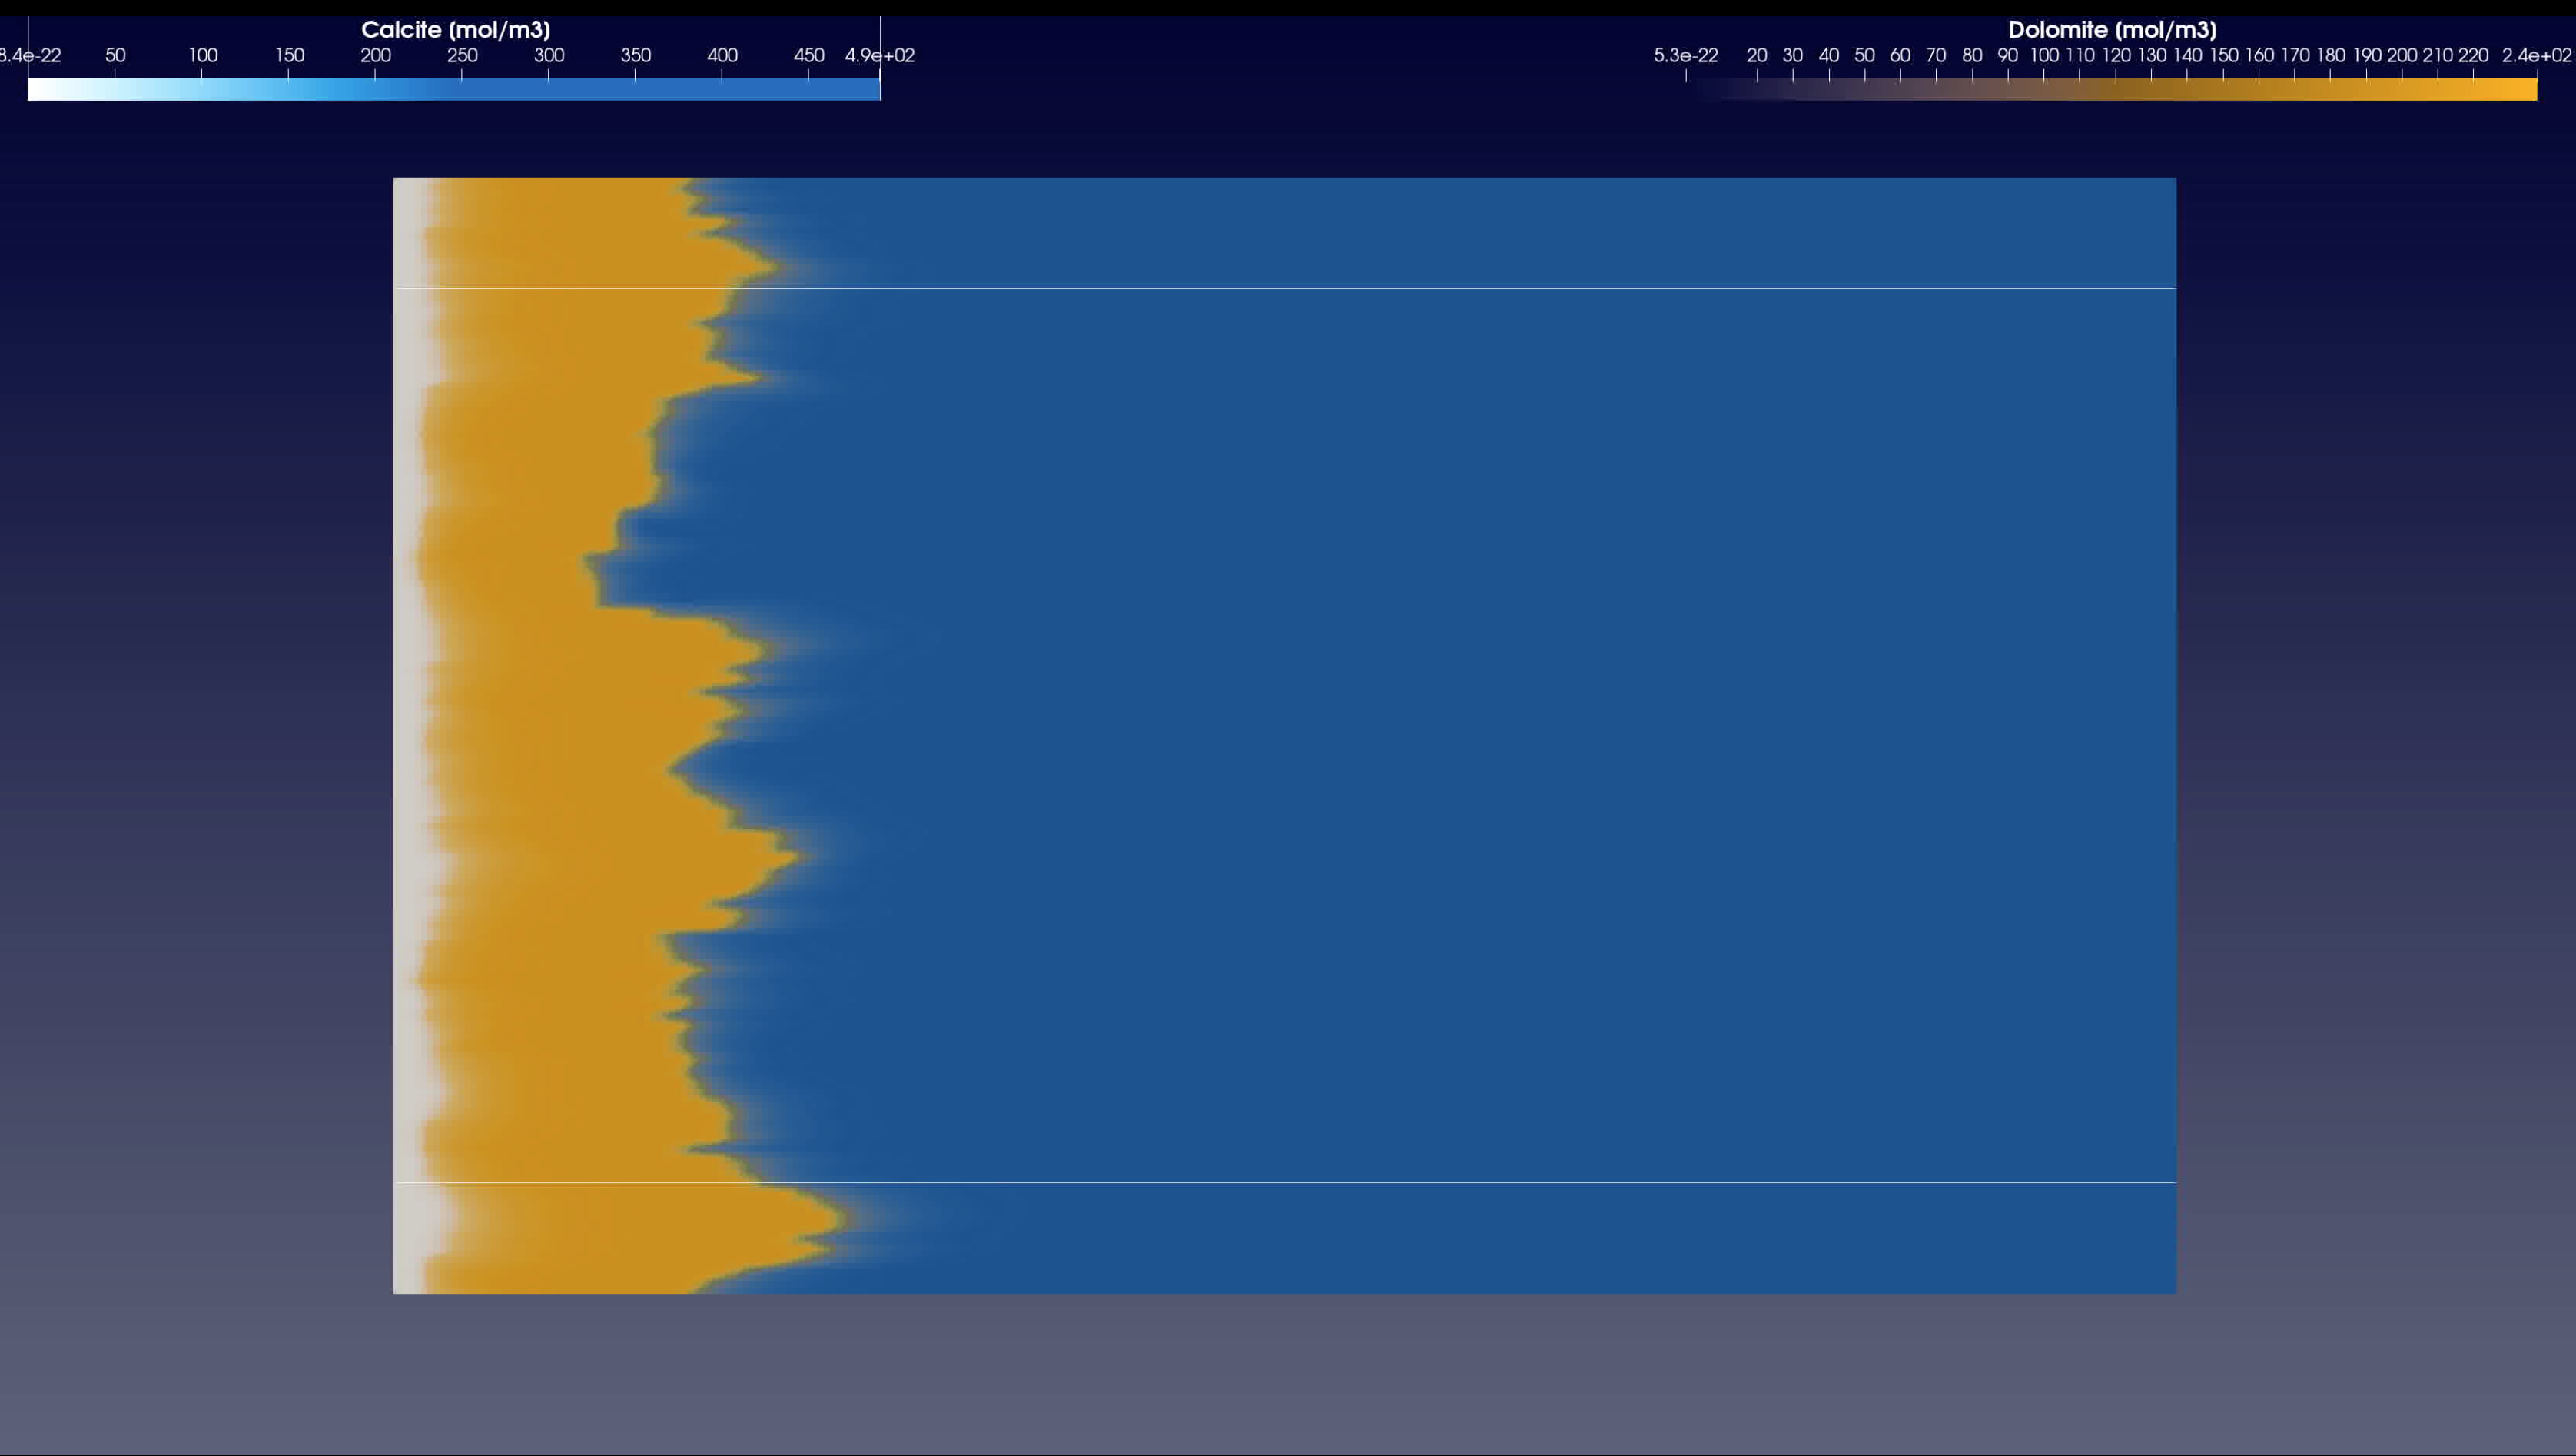
\includegraphics[width=0.45\textwidth, trim= 0 3cm 0 0, clip]{figures/rok/minerals-2s.png}}\\[-5pt]
\subfloat[]{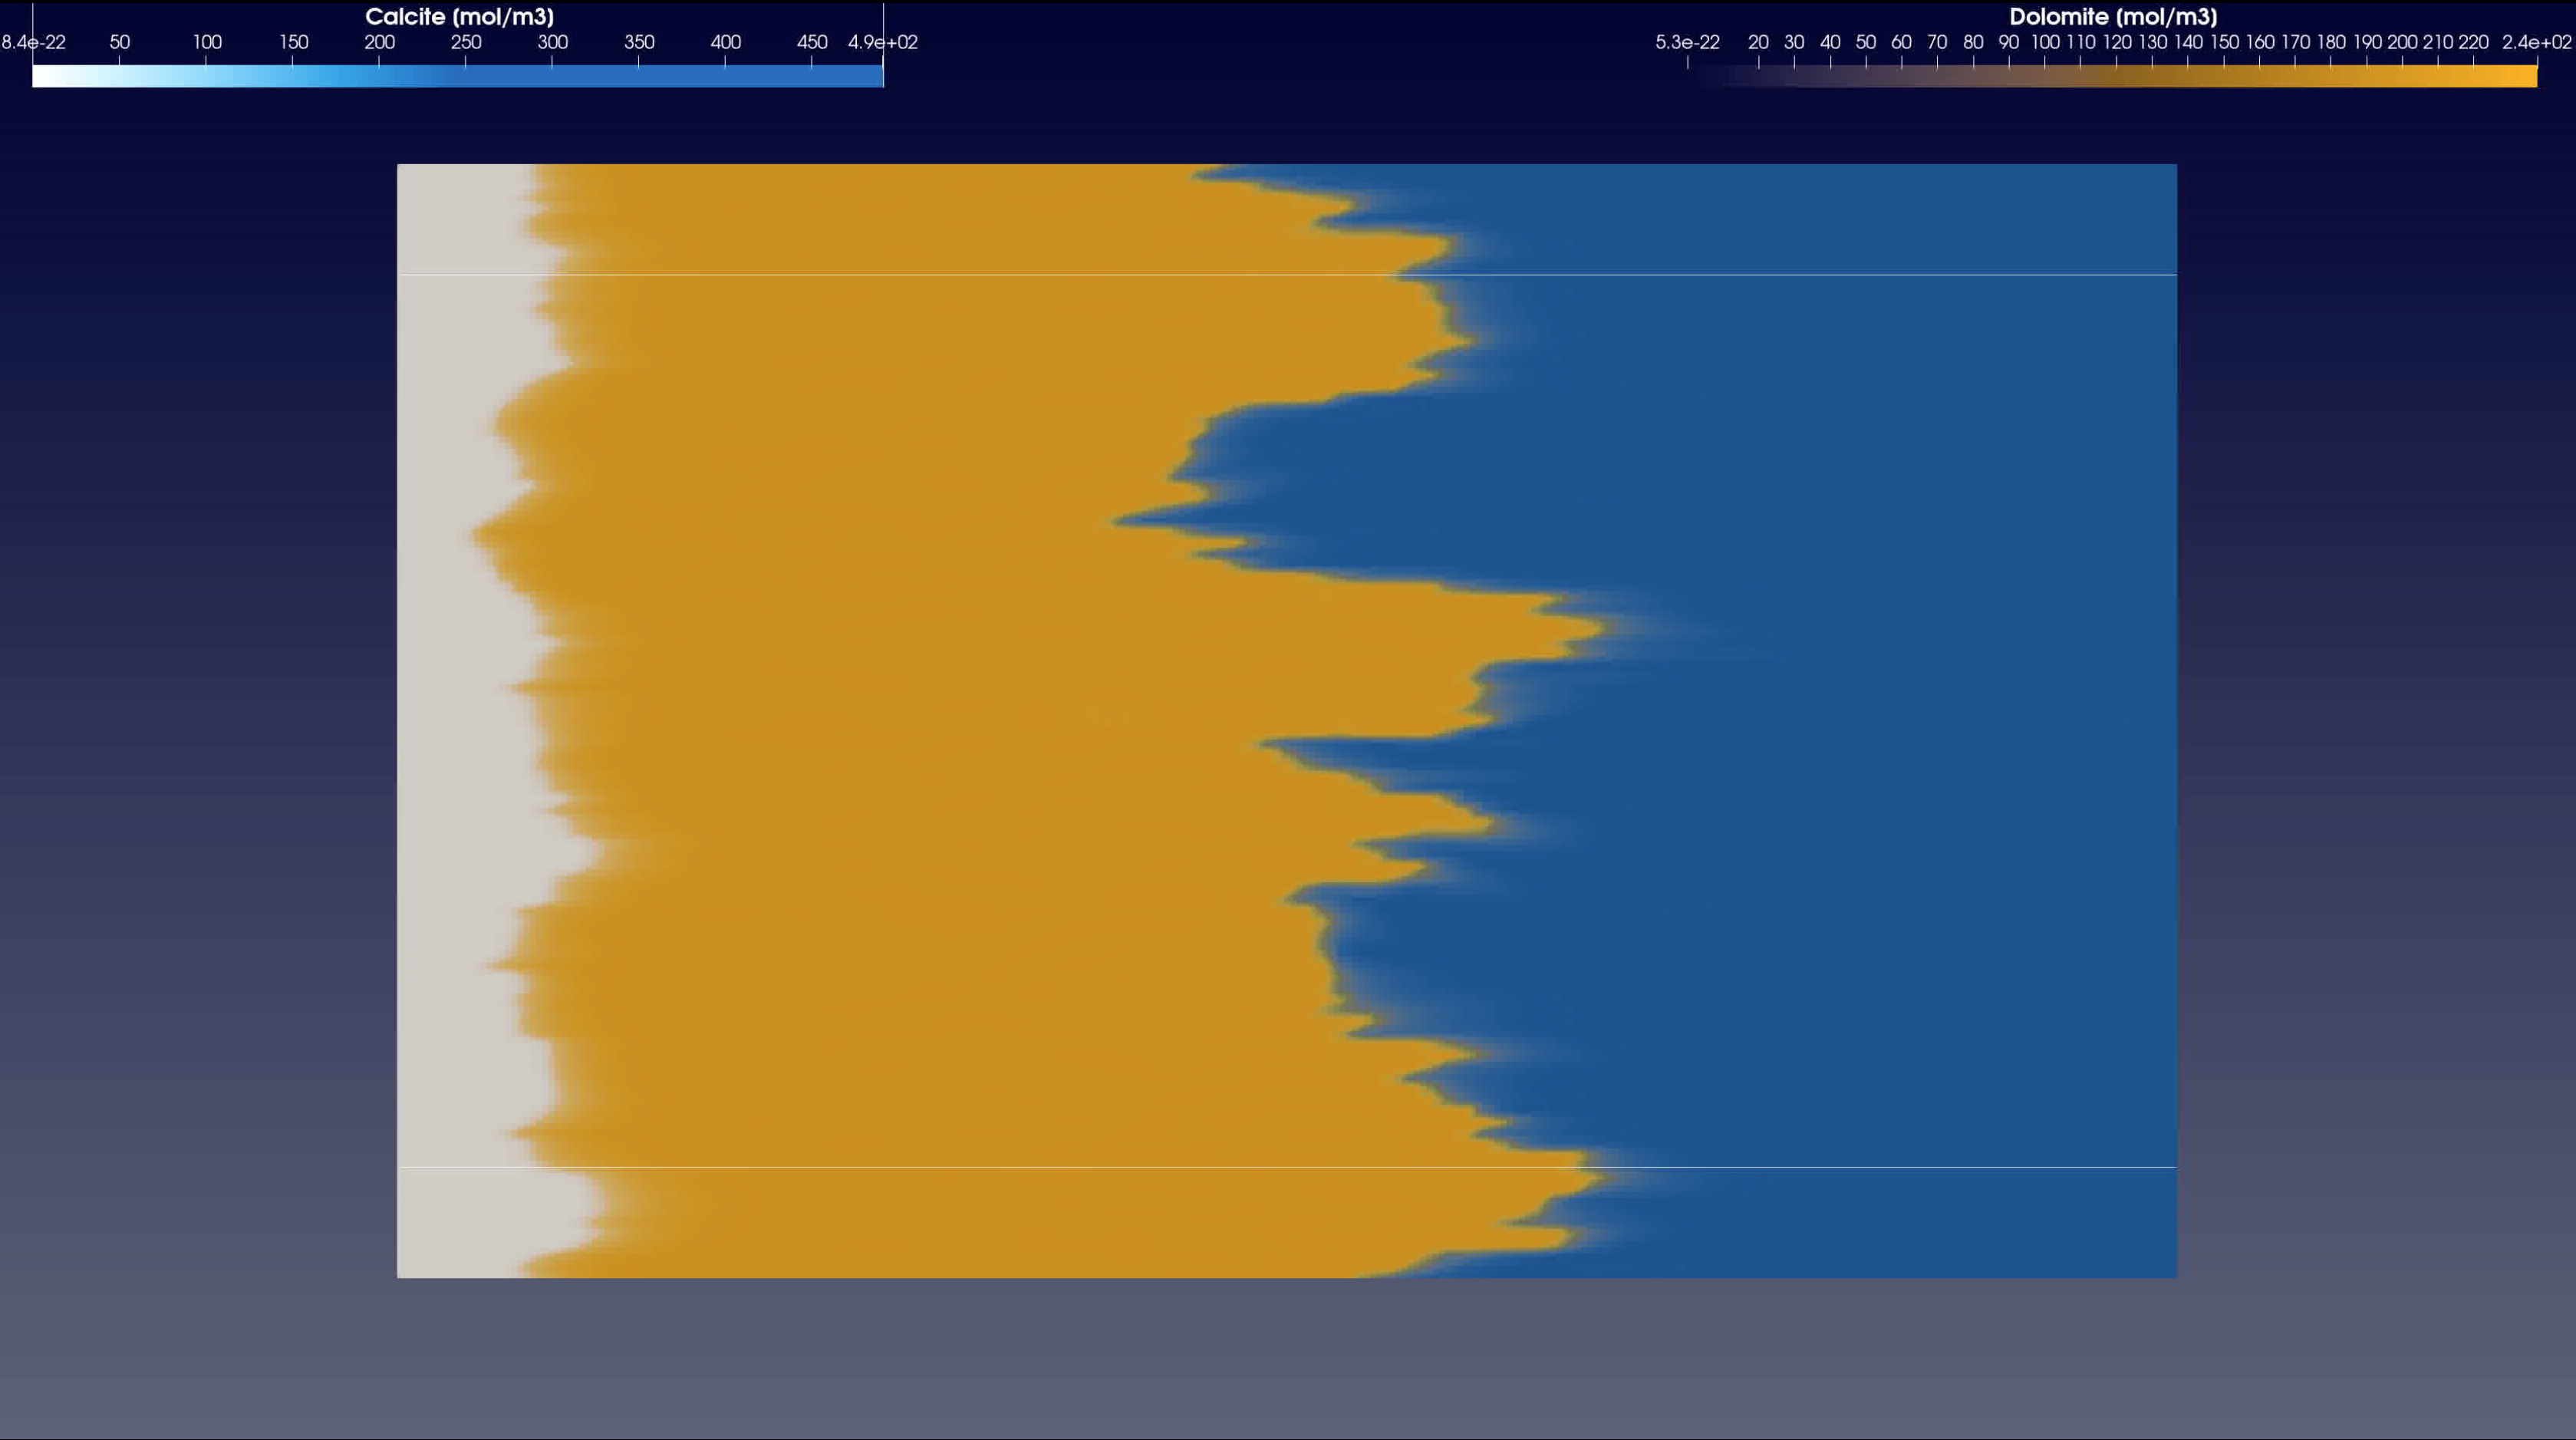
\includegraphics[width=0.45\textwidth, trim= 0 3cm 0 0, clip]{figures/rok/minerals-5s.png}}\quad
\subfloat[]{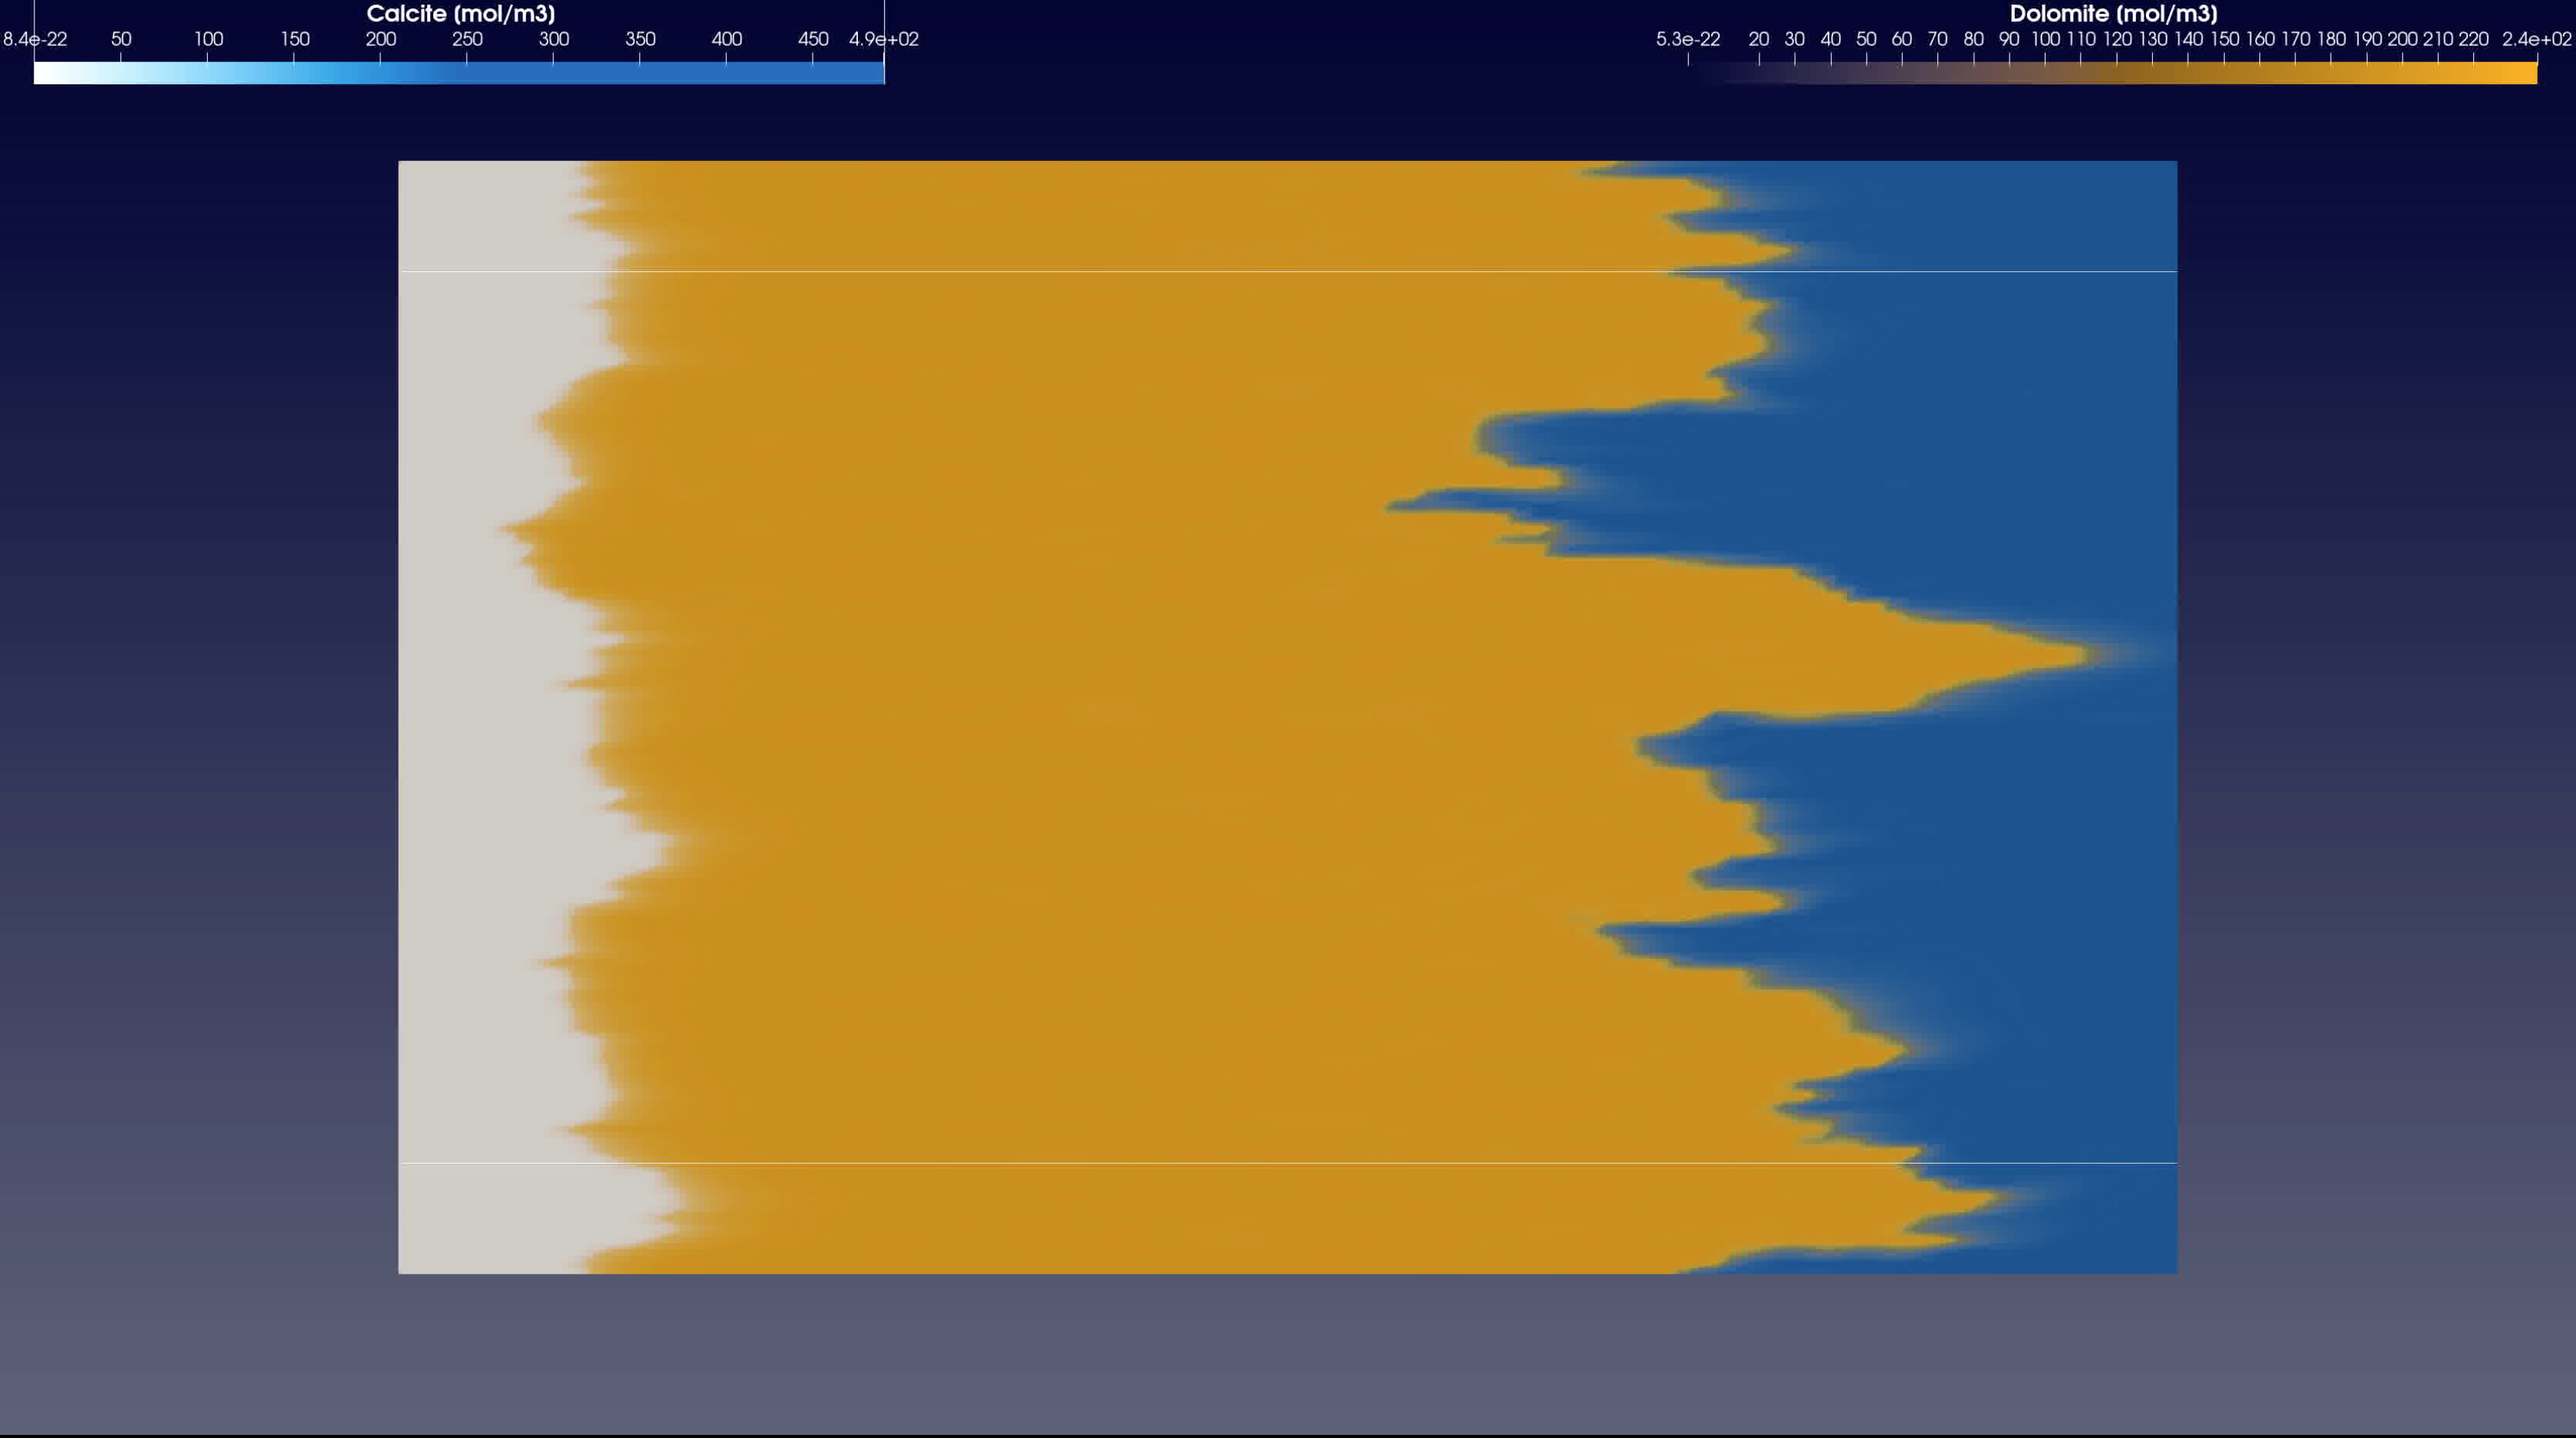
\includegraphics[width=0.45\textwidth, trim= 0 3cm 0 0, clip]{figures/rok/minerals-7s.png}}
\par\end{centering}
\caption{\label{fig:rok-minerals}
Mineral composition of the porous rock changing as an acidic aqueous fluid is injected on the left 
boundary at different time steps. Here, blue corresponds to Calcite, yellow depicts the concentration 
of Dolomite, and grey defines the regions of the rock with only Quartz.}
\end{figure}
%
\begin{figure}[!t]
\begin{centering}
\subfloat[]{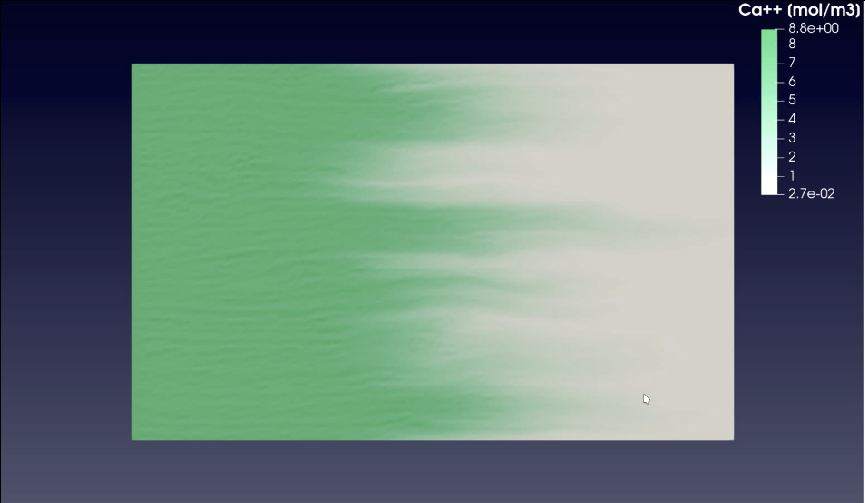
\includegraphics[width=0.45\textwidth, trim= 0 1cm 0 0, clip]{figures/rok/ca-ion.png}}\quad
\subfloat[]{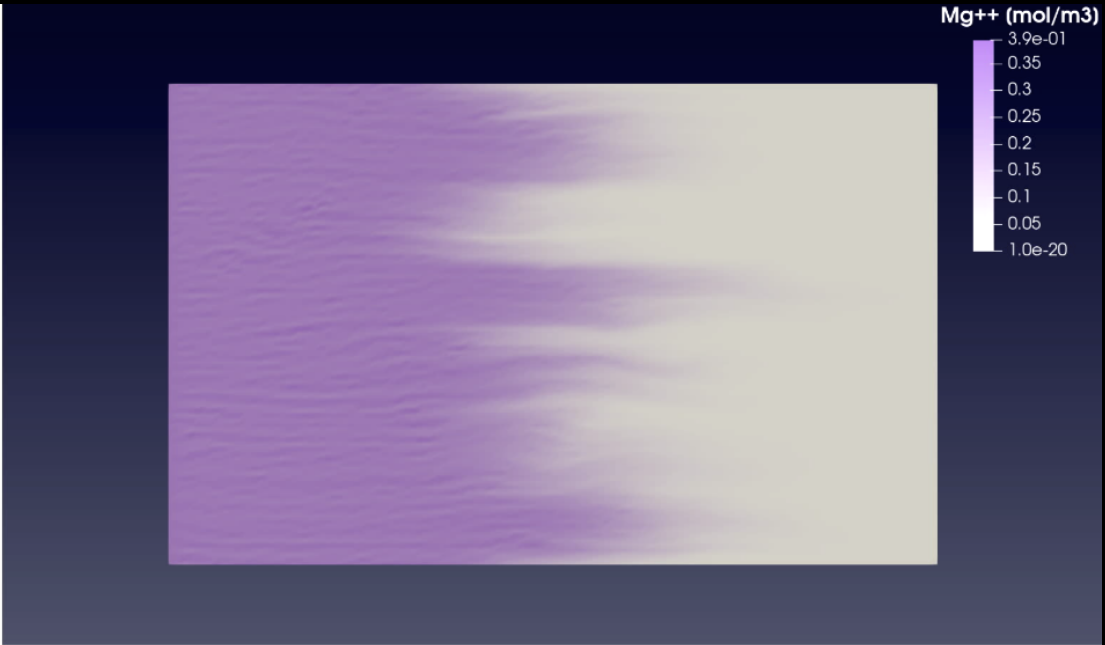
\includegraphics[width=0.45\textwidth, trim= 0 1cm 0 0, clip]{figures/rok/magnesium-ion.png}}\\[-5pt]
\subfloat[]{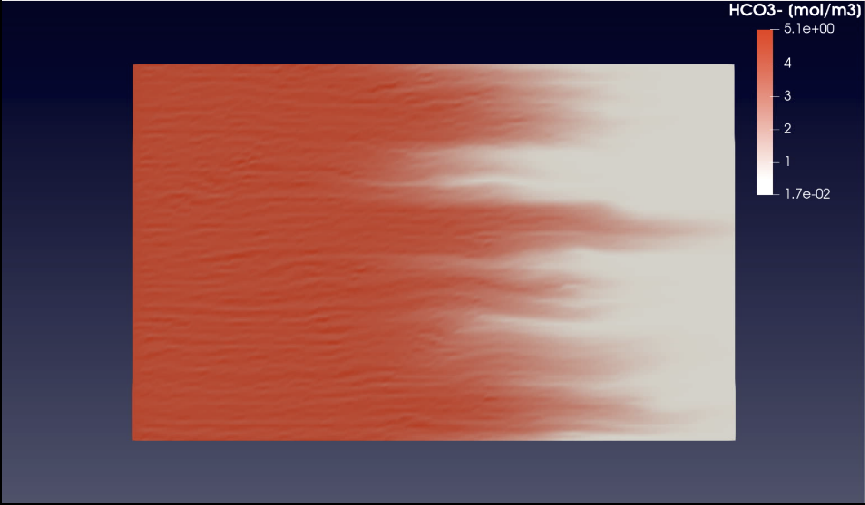
\includegraphics[width=0.45\textwidth, trim= 0 1cm 0 0, clip]{figures/rok/hco3-ion.png}}\quad
\subfloat[]{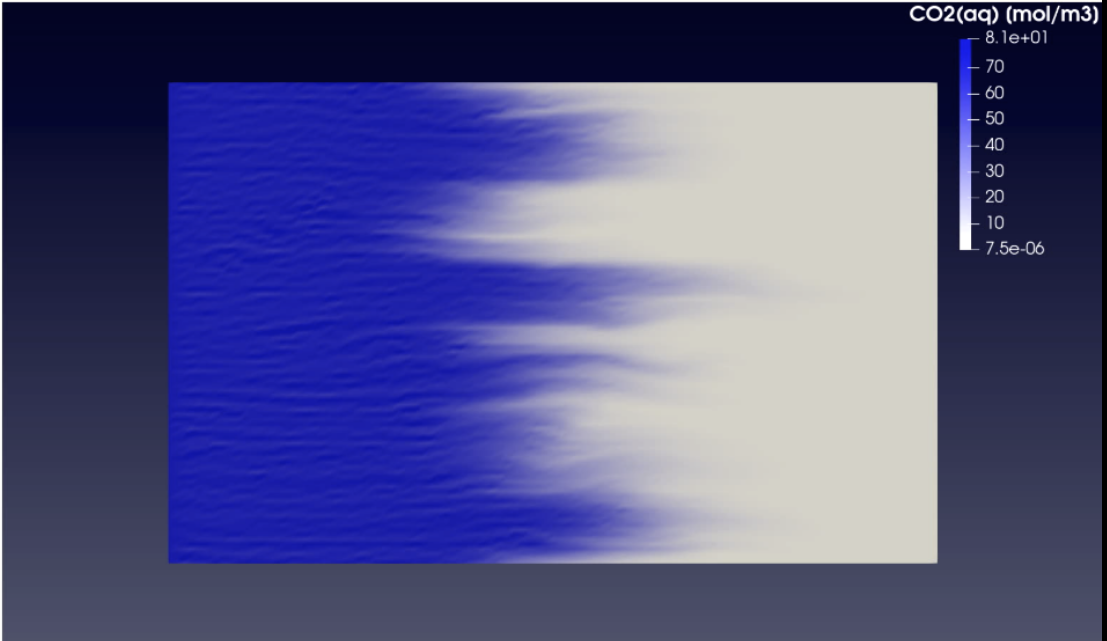
\includegraphics[width=0.45\textwidth, trim= 0 1cm 0 0, clip]{figures/rok/co2-aq.png}}
\par\end{centering}
\caption{\label{fig:rok-aqueous-species} Concentrations of (a) Ca$^{2+}$, (b) Mg$^{2+}$, 
(c) HCO$_3^{-}$ ions, and (d) CO$_2$(aq) (in ${\rm mol}/{\rm m}^3$)at certain moment of time of 
reactive transport.}
\end{figure}

%---------------------------------------------------------------------------------------------------%
Porosity change, resulting from reaction of rock minerals with the acidic aqueous fluid injected on 
the left boundary, is illustrated in Figure \ref{fig:rok-porosity}. We observe rather small change 
in porosity by 1.5 \%, from the initial value 1.1009 (see Figure \ref{fig:rok-porosity}(a)) till 
1.1180 (in red Figure \ref{fig:rok-porosity}(b)--(d)).
%
\begin{figure}[!t]
\begin{centering}
\subfloat[]{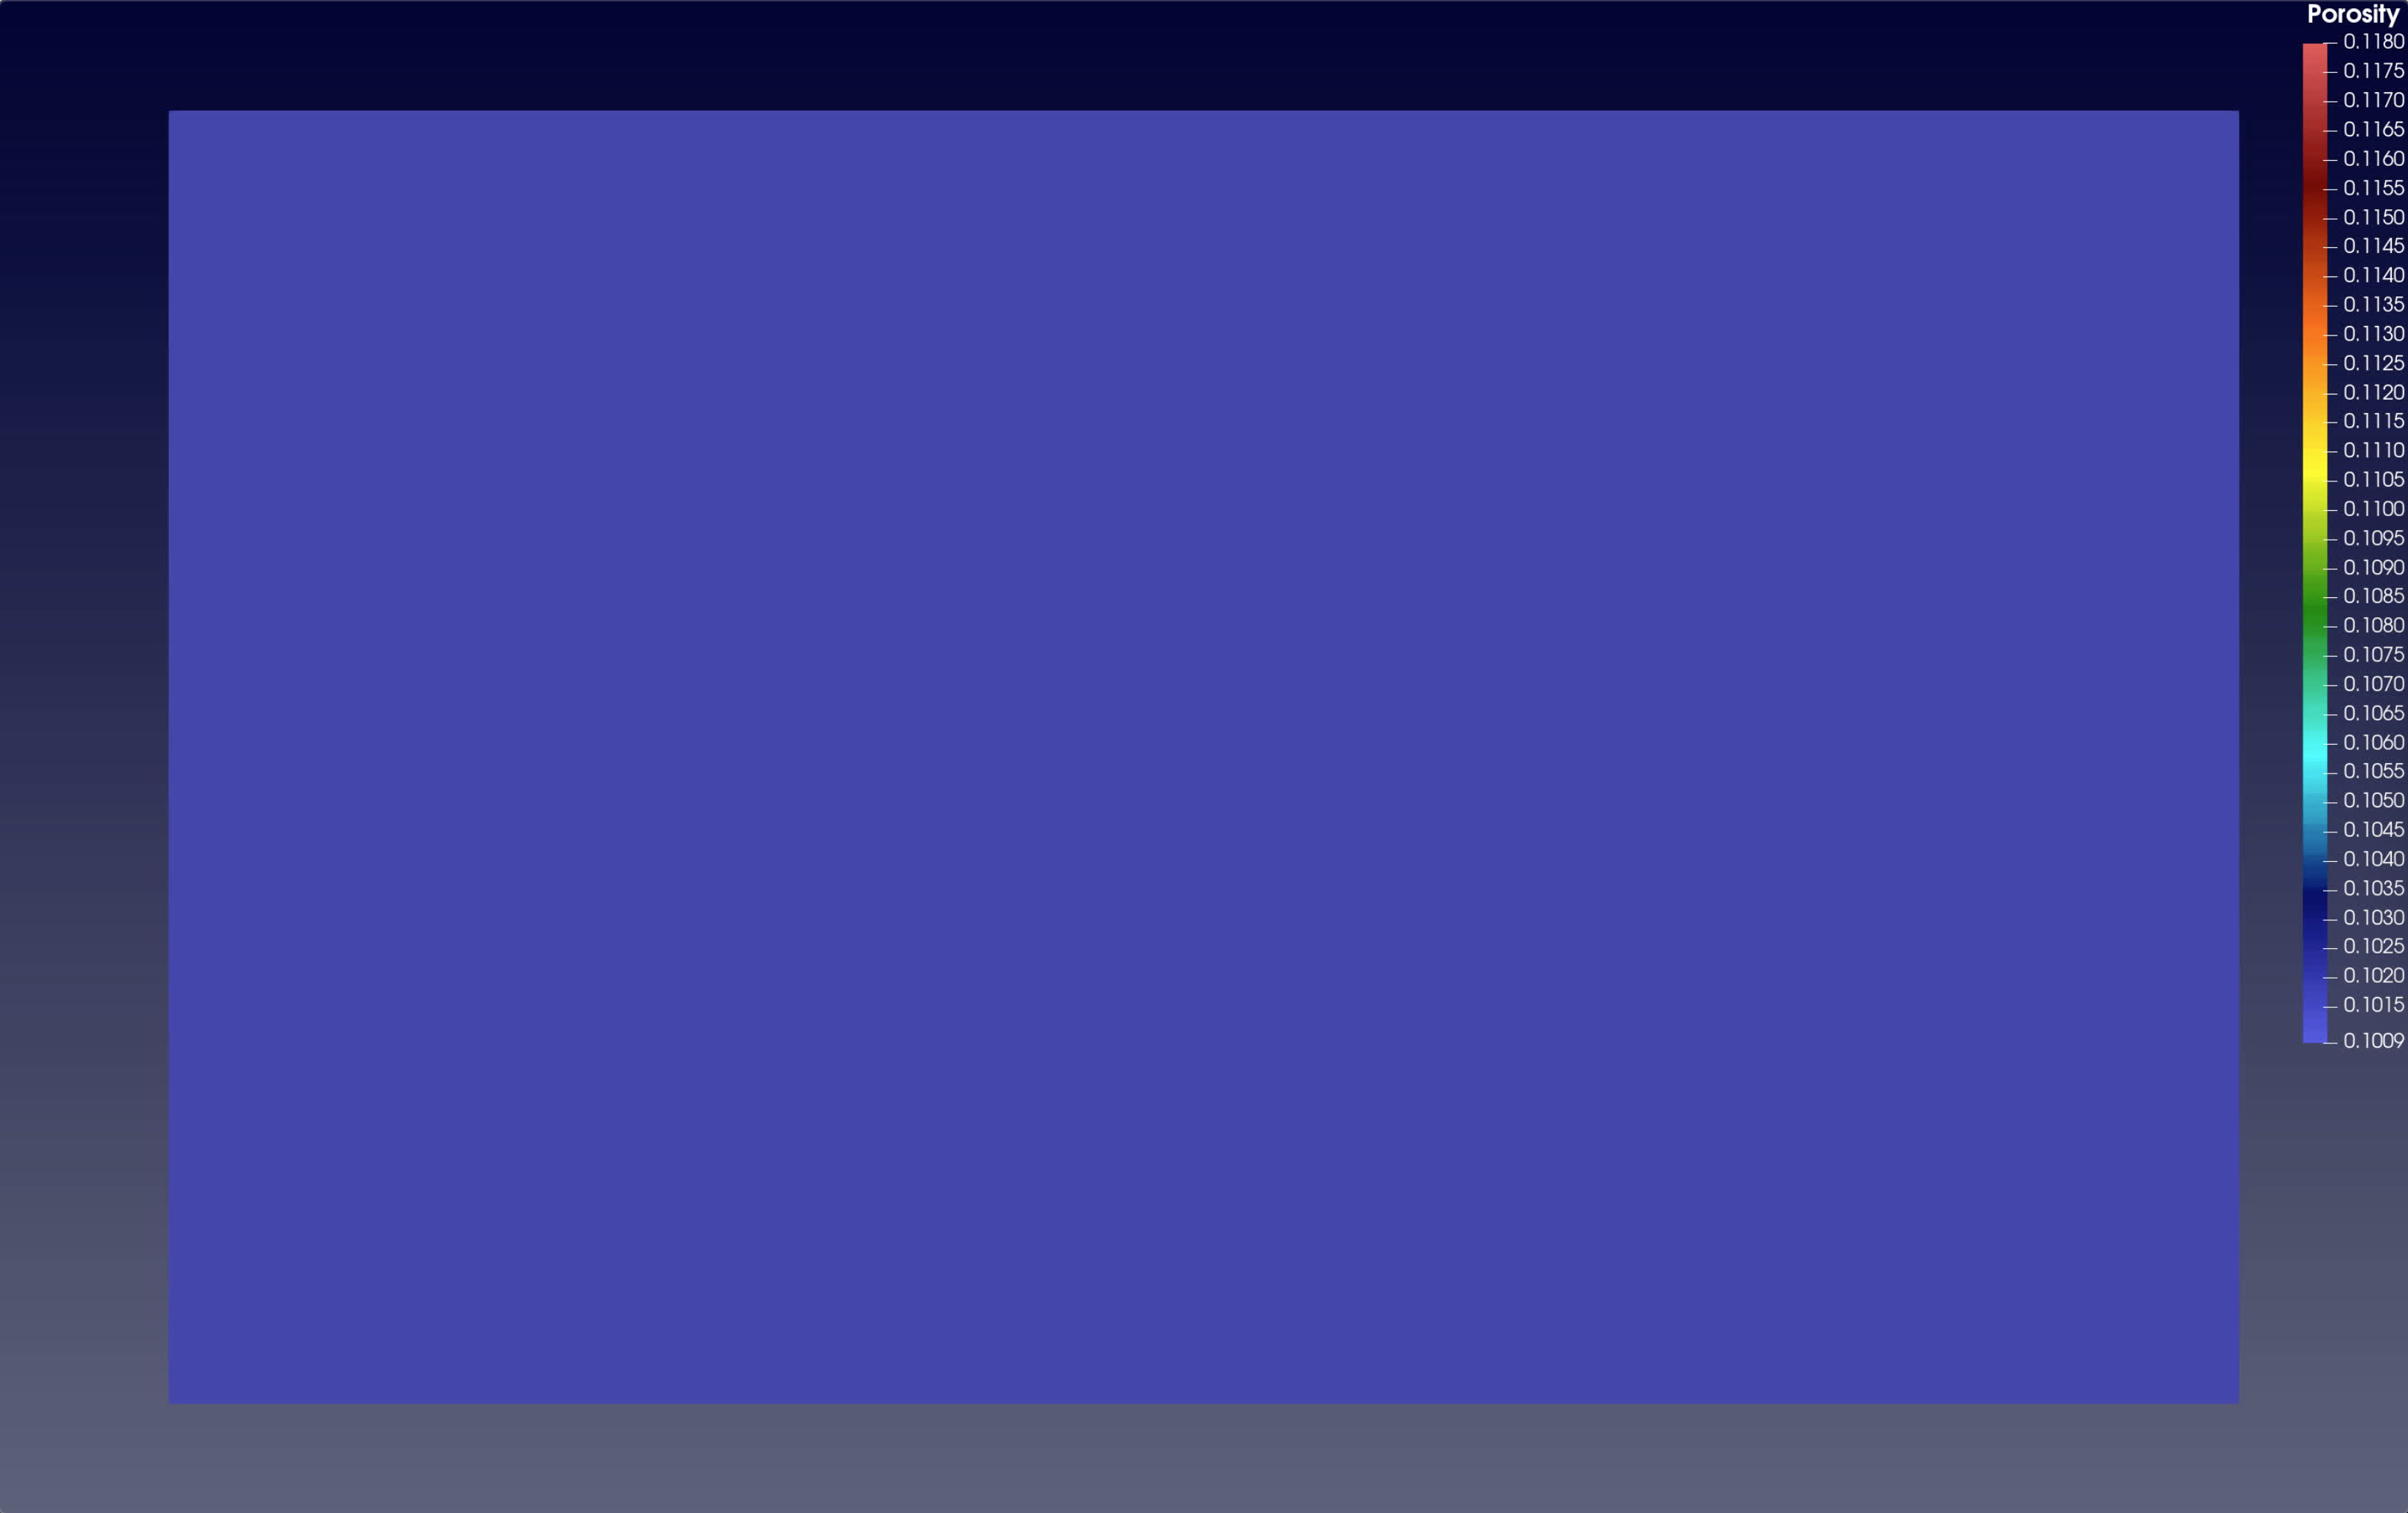
\includegraphics[width=0.45\textwidth, trim= 0 3cm 0 0, clip]{figures/rok/porosity-0s.png}}\quad
\subfloat[]{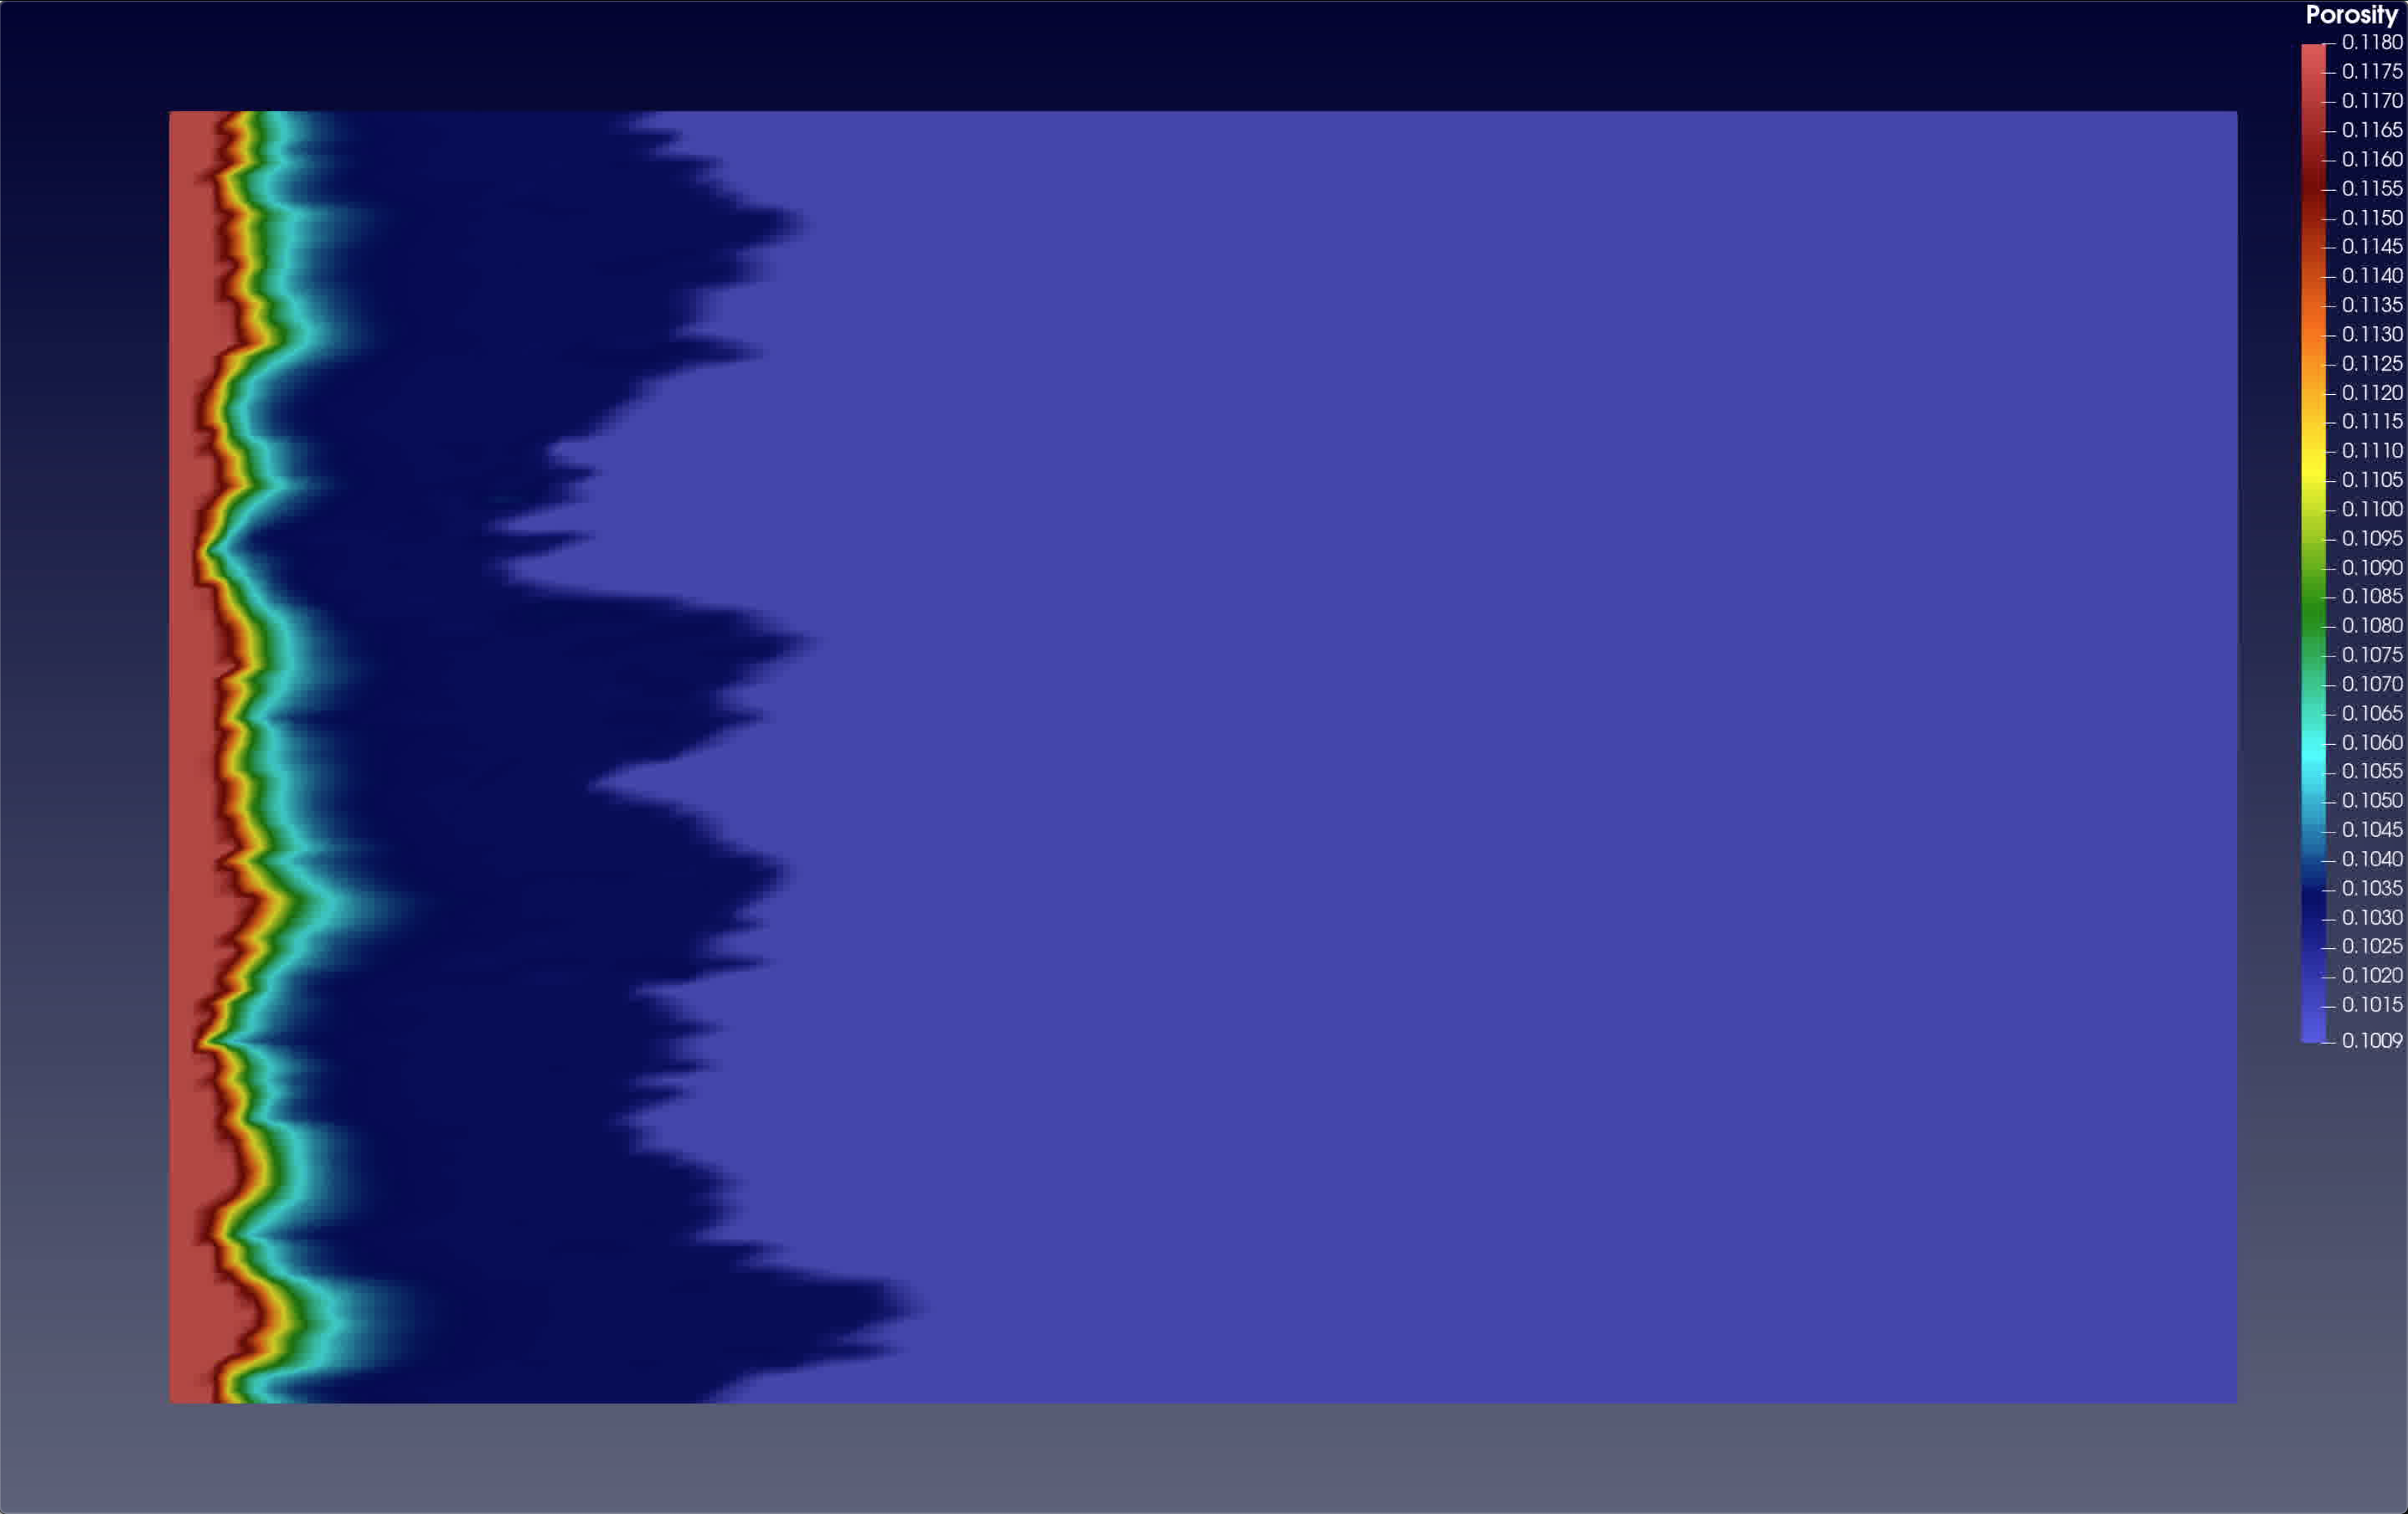
\includegraphics[width=0.45\textwidth, trim= 0 3cm 0 0, clip]{figures/rok/porosity-2s.png}}\\[-5pt]
\subfloat[]{\includegraphics[width=0.45\textwidth, trim= 0 3cm 0 0, clip]{figures/rok/porosity-5s.png}}\quad
\subfloat[]{\includegraphics[width=0.45\textwidth, trim= 0 3cm 0 0, clip]{figures/rok/porosity-7s.png}}
\par\end{centering}
\caption{\label{fig:rok-porosity}
Porosity changes as rock minerals react with the acidic aqueous fluid injected on the left boundary.}
\end{figure}



\section{Discussion and Conclusions\label{sec:Discussion-and-Conclusions}}

We suggest using a smart chemical equilibrium algorithm with on-demand learning
acceleration capabilities to substantially speedup reactive transport
simulations. For the specific problem investigated in this work, we
obtained a minimum speedup of 200~compared to the use of a conventional chemical
equilibrium algorithm. We note that this speedup may be specific to the
problem studied and the assumptions made about this particular chemical system.
Having said that, the system tested in this paper already consists of 36~species in 4~phases, with the
non-ideal thermodynamic behavior of the aqueous phase modeled using
the relatively expensive Pitzer activity model.

This substantial speedup is due to the capability of the smart chemical
equilibrium algorithm to learn from previous calculations during the reactive
transport simulation. This permits a quick and accurate prediction
of most subsequent speciation calculations with relatively similar input conditions (without
requiring iterative computations, such as when employing the Newton method).
The use of sensitivity derivatives is essential for this quick estimation.
These derivatives are calculated at the end of each on-demand learning operation,
using the automatic differentiation methods provided by \texttt{\href{http://autodiff.github.io}{autodiff}}
\citep{autodiff2018}. The estimation of new chemical speciation reactions is carried out by employing a
first-order Taylor expansion, using a previously learned (and stored) equilibrium
state as a reference point. This reference equilibrium state is searched
for by comparing the given input conditions for the new equilibrium
problem with the input conditions of previously solved problems in
the course of the reactive transport simulation (using the NN search).

We remark that the use of an on-demand learning strategy has advantages
compared to more common machine learning algorithms. In particular,
there is no need for an \emph{a priori training stage}, which can
impose many difficulties to modelers (who should not necessarily need
to understand how algorithms work, but rather what they can solve)
and interrupt their usual workflow. For modeling scenarios in which
it is not possible to have a reasonable insight in all possible geochemical
conditions that a chemical system may undergo during a simulation,
an a-priori training step can be challenging and compute-intensive. It can also require a comprehensive
training stage, generating extremely large amounts of data, most of which will likely never be needed. Moreover, a minimal change in modeling parameters
or configuration detail is enough to make that big data array obsolete
(e.g., a change of activity model, addition\slash removal of phases\slash species\slash reactions,
etc.), which can potentially compromise an exploratory modeling exercise
with many tested and analyzed setups. Last, but not the least, traditional,
statistics-based machine learning algorithms, applied to chemical
equilibrium calculations, neither understand the thermodynamic behavior
of stable phases nor can straightforwardly predict equilibrium
states that satisfy mass conservation of chemical elements and electric
charge.

We plan to assess the efficiency of the smart chemical equilibrium
algorithm under more complex geochemical and geological conditions.
This includes, for example, modeling radionuclide migration in nuclear
waste repositories, degradation processes in concrete, geothermal
energy systems, and carbon dioxide storage in geologic formations.
As future work, we also consider to further improve the NN search algorithm and the use of alternative acceptance criteria when
determining whether the estimated state has been determined accurately enough. Using
a similar on-demand learning strategy for speeding up chemical kinetics
calculations in reactive transport simulations is already underway.

This smart chemical equilibrium strategy with on-demand learning has been implemented in Reaktoro (\href{https://www.reaktoro.org}{reaktoro.org}), a unified
open-source framework for modeling chemically reactive systems.


\subsection{Plans}
%---------------------------------------------------------------------------------------------------%
A combination of tree-based and linear search algorithms is then needed. We can start with a linear 
search approach, since initially there are not many saved inputs of learned chemical equilibrium 
problems. Once a certain number of inputs have been saved, we construct a kd-tree. This approach 
should enable constructing more well-balanced kd-trees (i.e., trees, where sibling branches have a 
similar number of entries), and thus ensure faster search operations close to $\log_{2}(K)$ complexity.

Alternatively, \emph{locality-sensitive hashing}, the algorithm that hashes similar input items into 
the so-called ``buckets'' with high probability, can be considered. This technique can also be used 
for data clustering, since the space of stored $\mathcal{I}_e$ and $\mathcal{I}_k$ can be heavily 
clustered. This approach attempts to reduce the dimensional of $k$-dimensional data by providing 
low-dimensional representation of the latter while preserving relative distances between items.
%
\begin{comment}
TO CHECK:
https://github.com/simonemainardi/LSHash
https://github.com/salviati/slash
https://github.com/DBWangGroupUNSW/SRS
https://web.archive.org/web/20101203074412/http://www.vision.caltech.edu/malaa/software/research/image-search/
http://web.mit.edu/andoni/www/LSH/index.html
https://falconn-lib.org/
\end{comment}
%
We also plan to investigate retrieval of the reference states based on the ranking system, giving the 
higher priority of the most used chemical states to be considered first. This way, as soon as the acceptance 
element satisfies certain considered criterion, we can terminate the search process.  


\begin{comment}

We should investigate the following strategy. We impose a max number of stored entries (say, 300), organized in a contiguous memory data structure (std::vector, because we don't need to resize it). We periodically sort this vector by order of use (say, after each time step, we call a method SmartEquilibriumSolver::sortByUse(). During each time step, we allow new learning points to be saved at the tail of this vector (another option: they are stored in a separate vector, which would then be merged into the main search vector; in this merge process, some learning points may be discarded).
This would remove our dependency on kd-trees and nearest neighbors (which seems not to work well when high-dimensions are considered).

can be combined with using an efficient in-memory cache database or key-value store such as ArangoDB, Tarantool, or Redis


Residual-based acceptance algorithm. 

Reactive flows are all types of fluid flows with chemical reactions occouring within the fluid phase, at the interphase between different fluid phases or at interphases to solids. Gasphase combustion phenomena are the most important application of reactive flow modelling, while homogeneous combustion (gas-liquid or gas-solid) is still a minor research field. Simulation of reactive flows is getting more and more important, since they offer a possibility to gain insight to processes having harsh conditions, e.g. high temperture and pressure combustion. Additionally,  optimization of existing processes can be performed by modeling studies following design-of-experiment (DOE) approaches. In this way, the effort and costs for prototypes and field test can be reduced to a minimum.

However, modelling reactive systems is numerically expensive since the non-linear reaction kinetics leads to stiff-ODE systems in the species and energy conservation equations. Special solution algorithms, capable of handling these stiff systems of equations, are required to solve the equations. The best known stiff ODE solvers are the SIBS and RADAU5 algorithm.

Strategies to reduce the numerical effort to solve reactive flows include chemistry tabulation. Chemistry tabulation basically means that the solution of the given inital value problem (initial compostion, temperature, pressure) is stored. Subsequently, if similar starting values occur, the stored results are retrived and interpolated according to the differences in the starting values. These tabulation strategies differ depending on the employed combustion model. Some tabulation methods construct the tabulation on a predefined grid in the composition space, while others construt the tables "in-situ" during simulation run time.

Comment on the chemical properties evaluation.

\end{comment}

{\small
\section*{Acknowledgments}

This research project is funded by the Swiss National Science Foundation,
the Werner Siemens Foundation, and Shell. We thank these organizations
for their financial support.

\bibliographystyle{apalike-order-by-citation}
\bibliography{library,library-svetlana}

\appendix

\section{Reactive Transport Equations\label{sec:Reactive-Transport-Equations}}

Composition of each particle evolve according to the follwing set
of ODEs:

\begin{alignat*}{2}
\frac{\partial n_{i}}{\partial t} & =T(n_{i})+R(n_{i}) & \qquad & (i=1,\ldots,{\rm N}),
\end{alignat*}
where $T$ is the transport operator that consists of advection and
diffusion, $R$ is reaction operator. First order splitting method:
the solution advances from the time $t_{0}$ for a small time step
$\Delta t$ in the following order:
\begin{itemize}
\item solve transport equation, such that solution is denoted by $\overline{n}:$
%
\[
\begin{cases}
\frac{\partial n}{\partial t} & =T(n)\\
n(t_{0}) & =\boldsymbol{n_{0}}
\end{cases}
\]
\item from the initial condition $\overline{n}$, solve the reaction equation
to obtain $\tilde{n}$:
\[
\begin{cases}
\frac{\partial n}{\partial t} & =T(n)\\
n(t_{0}) & =\boldsymbol{\overline{n}}
\end{cases}
\]
\end{itemize}

The fundamental mass conservation equations for both fluid and solid
species are:
\begin{alignat}{2}
\frac{\partial n_{i}^{\rm f}}{\partial t}+\nabla\cdot(\boldsymbol{v}n_{i}^{\rm f}-D\nabla n_{i}^{\rm f}) & =r_{i}^{\rm f} & \qquad & (i=1,\ldots,{\rm N}^{\rm f}),\label{eq:cons-mass-fluid-species}\\
\frac{\partial n_{i}^{\rm s}}{\partial t} & =r_{i}^{\rm s} &  & (i=1,\ldots,{\rm N}^{\rm s}),\label{eq:cons-mass-solid-species}
\end{alignat}
where $n_{i}^{\rm f}$ and $n_{i}^{\rm s}$ are the \emph{bulk
concentration} of the $i$th fluid and solid species (in mol/m$^{3}$),
respectively; $\boldsymbol{v}$ is the fluid pore velocity (in m/s);
$D$ is the diffusion coefficient of the fluid species (in m$^{2}$/s);
$r_{i}^{\rm f}$ and $r_{i}^{\rm s}$ are the rates of production\slash consumption
of the $i$th fluid and solid species (in mol\slash s), respectively,
due to chemical reactions; and ${\rm N}^{\rm f}$ and ${\rm N}^{\rm s}$
are the numbers of fluid and solid species, respectively. Note that
the above equations assume a single fluid phase and common diffusion
coefficients for all fluid species.

By partitioning the species as fluid and solid species, the formula
matrix $A$ can be conveniently represented as:
\begin{equation}
A=\begin{bmatrix}A^{\rm f} & A^{\rm s}\end{bmatrix},
\end{equation}
where $A^{\rm f}$ and $A^{\rm s}$ are the formula matrices
of the fluid and solid partitions (i.e., the matrices constructed
from the columns of $A$ corresponding to fluid and solid species).
The concentrations of elements in both fluid and solid partitions
$b_{j}^{\rm f}$ and $b_{j}^{\rm s}$ can then be calculated
from the species concentrations in the same partition using: 
\begin{alignat}{2}
b_{j}^{\rm f} & =\sum_{i=1}^{{\rm N}^{\rm f}}A_{ji}^{\rm f}n_{i}^{\rm f} & \qquad & (j=1,\ldots,{\rm E})\\
\shortintertext{and}b_{j}^{\rm s} & =\sum_{i=1}^{{\rm N}^{\rm s}}A_{ji}^{\rm s}n_{i}^{\rm s} &  & (j=1,\ldots,{\rm E}).
\end{alignat}

Recall that the rates of production of the species $r_{i}^{\rm f}$
and $r_{i}^{\rm s}$ are exclusively due to chemical reactions.
Let $r_{i}$ denote the rate of production\slash consumption of the
$i$th species in the system (i.e., using global index, and not a
local index within the fluid or solid partition). From the mass conservation
condition for the elements (chemical elements and electrical charge),
it follows that:
\begin{equation}
\underset{\substack{{\rm rate of production}\\
{\rm  of element \ensuremath{j}}
}
}{\underbrace{\sum_{i=1}^{{\rm N}}A_{ji}r_{i}}}=\underset{\substack{{\rm rate of production}\\
{\rm  of element \ensuremath{j} in}\\
{\rm the fluid partition}
}
}{\underbrace{\sum_{i=1}^{{\rm N}^{\rm f}}A_{ji}^{\rm f}r_{i}^{\rm f}}}+\underset{\substack{{\rm rate of production}\\
{\rm  of element \ensuremath{j} in}\\
{\rm the solid partition}
}
}{\underbrace{\sum_{i=1}^{{\rm N}^{\rm s}}A_{ji}^{\rm s}r_{i}^{\rm s}}}=\quad0,
\end{equation}
which is the mathematical statement for the fact that \emph{elements
are neither created nor destroyed} during chemical reactions. We can
combine this result with equations (\ref{eq:cons-mass-fluid-species})
and (\ref{eq:cons-mass-solid-species}) to derive the following conservation
equations for the elements:
\begin{equation}
\frac{\partial b_{j}^{\rm s}}{\partial t}+\frac{\partial b_{j}^{\rm f}}{\partial t}+\nabla\cdot(\boldsymbol{v}b_{j}^{\rm f}-D\nabla b_{j}^{\rm f})=0\qquad(j=1,\ldots,{\rm E}).
\end{equation}

Assume that all species, fluid and solid, are in \emph{local chemical
equilibrium everywhere, at all times}. One can then perform \emph{operator
splitting steps} to solve the fundamental mass conservation equations
(\ref{eq:cons-mass-fluid-species}) and (\ref{eq:cons-mass-solid-species})
to calculate the concentrations of the species, $n_{i}$, over time.
Let $k$ denote the current \emph{time step} and $\Delta t$ the \emph{time
step length} used in the discretization of the time derivative terms.
The operator splitting steps at the $k$th time step are:


\begin{enumerate}[wide, labelwidth=!, labelindent=0pt]
\item[\textbf{Step 1)}] We consider (Eq.~\ref{eq:transport}) without
${\partial b_{j}^{\text{s}}}/{\partial t}$ term and
compute an intermediate approximation of element concentrations in the fluid
partition $\tilde{b}^{\text{f}}=(\tilde{b}_{1}^{\text{f}},\ldots,\tilde{b}_{\mathrm{E}}^{\text{f}})$
at time $t_{k+1}$ using
\begin{equation}
\frac{\tilde{b}_{j}^{\text{f},k+1}-\tilde{b}_{j}^{\text{f},k}}{\Delta t}+\nabla\cdot(\boldsymbol{v}\tilde{b}_{j}^{\text{f},k+1}-D\nabla\tilde{b}_{j}^{\text{f},k+1})=0\qquad(j=1,\ldots,\text{E}),\label{eq:fluid-element-transport}
\end{equation}
%
with the following flux boundary condition at $x=x_{L}$ (on the left
boundary inlet face, where we inject the CO$_{2}$-saturated brine):
\begin{equation}
-(\boldsymbol{v}\tilde{b}_{j}^{{\rm f},k+1}-D\nabla\tilde{b}_{j}^{{\rm f},k+1})\cdot\textbf{n}_{L}=v\phi_{L}\hat{b}_{j,L}
\qquad(j=1,\ldots,{\rm E}),
\end{equation}
%
where subscript $L$ denotes the left boundary at $x=x_{L}$,
$\textbf{n}_{L}$ is the normal vector on the inflow face,
$\phi_{L}$ is the current porosity at $x=x_{L}$ (which changes with time),
and $\hat{b}_{j,L}$ (in $\mathrm{mol/m_{\mathrm{fluid}}^{3}}$) is the imposed concentration of the $j$th element in the injected brine.
%
To match the units of concentrations of the elements in the fluid $[b_{j}]=\mathrm{mol/m_{\mathrm{bulk}}^{3}}$
and the imposed concentration $[\hat{b}_{j,L}]=\mathrm{mol/m_{\mathrm{fluid}}^{3}}$ , we need to
multiply it by $\phi_{L}$ ($\mathrm{m_{fluid}^{3}/m_{bulk}^{3}}$). The right face 
pf the rock is considered free. 
%
To discretize the above partial differential equations in space, a finite volume method is applied.
The time integration uses an implicit scheme for both advection and diffusion.
%
\item[\textbf{Step 2)}] Update the total concentrations of each element $b_{j}$ using
the previously computed intermediate concentrations of each element in the fluid $b_{j}^{\mathrm{f}}$:
%
\begin{equation}
b_{j}^{k+1}=\tilde{b}_{j}^{\text{f},k+1}+b_{j}^{\text{s},k}.
\end{equation}
%
Note that each element concentration in the solid partition $b_{j}^{\mathrm{s}}$
remains constant during the transport calculations in the previous
step.
\item[\textbf{Step 3)}] Calculate the concentrations of the species, $n_{i}^{k+1}$, in
each mesh cell. For this, use as inputs the temperature and pressure
values of the cell together with the \emph{updated local concentrations
of elements}, $b_{j}^{k+1}$, from the previous step. Let the on-demand
learning algorithm determine, in each cell, if it needs to fully solve
the current equilibrium problem or if it can quickly estimate the
species amounts $n=(n_{1},\ldots,n_{\mathrm{N}})$ using a previously
learned problem with similar inputs.
\end{enumerate}
 
\section{Chemical Kinetics Equations \label{subsec:Chemical-kinetics-equations}}

%---------------------------------------------------------------------------------------------------%
The \textbf{principle of mass conservation} $\frac{dn}{dt}=q$ yields 
%
\[
\frac{db}{dt}=\frac{db_{e}}{dt}+\frac{db_{k}}{dt}=Aq=A_{e}q_{e}+A_{k}q_{k},
\label{eq:mass-concervation}
\]
%
i.e., the amounts of the elements in the system $b$ vary according to the amounts of elements 
entering/leaving the system as a result of the given inflow/outflow rates of chemical species $q$. 
%
At the same time, Eq. \ref{eq:kinetics} for kinetic species yields
%
\begin{align}
\frac{db_{k}}{dt} & =A_{k}\nu_{k}^{T}r+A_{k}q_{k}.
\label{eq:kinetics-with-b}
\end{align}
%
%---------------------------------------------------------------------------------------------------%
Combination of Eq. \ref{eq:mass-concervation} and \ref{eq:kinetics-with-b} leads to
%
\[
\frac{db_{e}}{dt}=A_{e}q_{e}-A_{k}\nu_{k}^{T}r.
\]
%
Using the \emph{stoichiometric balance condition} $A\nu^{T}=A_{e}\nu_{e}^{T}r+A_{k}\nu_{k}^{T}r=0$, 
which can be rewritten as $-A_{k} \, \nu_{k}^{T} \, r = A_{e}  \, \nu_{e}^{T} \, r$, we arrive at
\[
\frac{db_{e}}{dt} = A_{e}q_{e}-A_{k}\nu_{k}^{T}r = A_{e}(q_{e}+\nu_{e}^{T}r).
\]
%
This means that the \emph{chemical state of a system} is govern by the following differential-algebraic 
problem
%
\[
\begin{cases}
\frac{dn_{k}}{dt}=\nu_{k}^{T}r+q_{k} & t>0\\
\frac{db_{e}}{dt}=A_{e}(q_{e}+\nu_{e}^{T}r) & t>0\\
n_{e}=\varphi(b_{e}) & t>0\\
n_{k}=n_{k}^{\circ} & t=0\\
n_{e}=n_{e}^{\circ} & t=0\\
b_{e}=A_{e}n_{e}^{\circ} & t=0
\end{cases},
\]
where $n=(n_{e}^{\circ},n_{k}^{\circ})$ is given initial condition.

Open system:
%
\begin{align*}
\frac{dn}{dt} & =\nu^{T}r+q & t>0,\\
n & =n^{\circ} & t=0,
\end{align*}
where $r_{m}=r_{m}(T,P,n,a)$ is nonlinear dependent from $n$
\begin{itemize}
\item $q\in R^{N}$is a \emph{vector of inflow rates},
\item $n\in R^{N}$is a\emph{ vector of composition} of the chemical system,
\item $a\in R^{N}$is \emph{species activities}.
\end{itemize}
%System of non-linear ODEs due to the non-linear dependence of $r_{m}=r_{m}(T,P,n,a)$ from $n$.\\

\textbf{\textcolor{brown}{Rate laws}}\\
\textbf{\textcolor{brown}{}}\\
\textcolor{black}{General }\textbf{\textcolor{black}{rate law}}\textcolor{black}{{}
for crystal growth and mineral dissolution (allows to model several
kinetic mineral mechanisms such as acid, neutral, base, carbonate,
and so forth) / mineral dissolution and precipitation
\begin{align*}
r_{m}(T,P,n) & :=n_{m}\sigma_{m}\sum_{i}M_{m,i}(T,P,n),\\
M_{m,i}(T,P,n) & :={\rm sgn}(1-\Omega)k_{m,i}|1-\Omega^{p_{i}}|^{q_{i}}\prod_{j}a_{j}^{\xi_{j}}\prod_{g}P_{g}^{\eta_{g}},
\end{align*}
where}
\begin{itemize}
\item $n_{m}$ is the \emph{current molar amount} of the mineral, either
dissolving or precipitating;
\item $\sigma_{m}$ is current specific\emph{ reactive surface area} of
the mineral (m2 / mol);
\item \textcolor{black}{$\Omega:=\frac{1}{K_{m}}\prod_{i=1}^{N}a_{i}^{\nu_{i}}$
is current }\textcolor{black}{\emph{saturation index}}\textcolor{black}{{}
of the mineral defined via activity product (and }$\nu_{i}$\emph{
stoichiometric coefficient} of the $i$-th ionic species\textcolor{black}{)
and }\textcolor{black}{\emph{equilibrium constant}}\textcolor{black}{{}
$K_{m}$}
\item \textcolor{black}{$k_{m,i}$ is the }\textcolor{black}{\emph{rate
constant}}\textcolor{black}{{} of the $i$th mineral reaction,$k_{m,i}:=k_{m,i}^{\circ}\exp\bigg[-\frac{E_{m,i}}{R}(\frac{1}{T}-\frac{1}{298.15})\bigg]$
(Arrhenius equation) with $k_{m,i}^{\circ}$ as the }\textcolor{black}{\emph{reaction
rate}}\textcolor{black}{{} constant at 25 °C, the }\textcolor{black}{\emph{activation
energy}}\textcolor{black}{{} $E_{m,i}$; and the }\textcolor{black}{\emph{universal
gas constant }}\textcolor{black}{$R$;}
\item \textcolor{black}{$p_{i}$ and $q_{i}$ are }\textcolor{black}{\emph{empirical
exponents}}\textcolor{black}{{} used to fit the rate law and control
how saturation affects the mineral rate; and}
\item \textcolor{black}{$a_{j}$ is the }\textcolor{black}{\emph{activity}}\textcolor{black}{{}
of the $j$th species, $P_{g}$ is the }\textcolor{black}{\emph{partial
pressure}}\textcolor{black}{{} of the $g$th gaseous species; and}
\item \textcolor{black}{$\xi_{j}$and $\eta_{g}$ are the exponents of the
catalysts (>0) and inhibitors (<0).}
\end{itemize}
\textbf{\textcolor{brown}{Partial equilibrium}}\\
\textbf{\textcolor{brown}{}}\\
Partition to:
\begin{itemize}
\item \emph{slow / kinetics} reaction (corresponding kinetics species) 
\[
0\rightleftharpoons\sum_{i=1}^{N}\nu_{ij}^{k}\alpha_{i},j=1,...,M_{k}
\]
with$\boldsymbol{\nu}_{k}\mathbb{\in M}^{M_{k}\times N}$, which include
kinetic $\boldsymbol{\nu}_{kk}\mathbb{\in M}^{M_{k}\times N_{k}}$
and equilibrium species $\boldsymbol{\nu}_{ke}\mathbb{\in M}^{M_{k}\times N_{e}}$
\item \emph{fast / equilibrium} reaction (corresponding equilibrium species)
\end{itemize}
\textcolor{brown}{Question: Isn't stoichometry just for the reactions?}

Then,
\begin{itemize}
\item $n_{e}$ and $n_{k}$ are the vectors of the amounts of the equilibrium
and the kinetic species, respectively;
\item $b_{e}$ and $b_{k}$ are the vectors of the amounts of the elements
such that 
\[
n=\begin{bmatrix}n_{e}\\
n_{k}
\end{bmatrix}:\mathbb{R}^{N}\rightarrow\mathbb{R}^{N}
\]
\item $A_{e}$ and $A_{k}$ are matrices of the equilibrium and kinetic
species $A=\begin{bmatrix}A_{e}\,A_{k}\end{bmatrix}$and
\item $\nu_{e}$ and $\nu_{k}$ are matrices formed from the \textbf{columns}
of the stoichiometric matrix $\nu=\begin{bmatrix}\nu_{e}\,\nu_{k}\end{bmatrix}$
\end{itemize}
Dependence of $n_{e}$ from $b_{e}$ is prescribed by the chemical
equilibrium function $n_{e}=\varphi(b_{e}),\varphi:\mathbb{R}^{E}\rightarrow\mathbb{R}^{N}$
that encapsulates the specific algorithmic steps to solve the equilibrium
problem
\[
\varphi(b_{e}):={\rm argmin}_{n_{e}}G_{e}=n_{e}^{T}\mu_{e}\quad\mbox{subject to}\quad\begin{cases}
A_{e}n_{e} & =b_{e}\\
n_{e} & \geq0
\end{cases}.
\]

The amounts of the kinetic species, $n_{k}$
\begin{align*}
\frac{dn_{k}}{dt} & =\nu_{k}^{T}r+q_{k} & t>0,\\
n_{k} & =n_{k}^{\circ} & t=0,
\end{align*}
where
\begin{itemize}
\item $r$ are the \emph{rates} of the kinetically controlled reactions;
\item $q_{k}$ denotes the\emph{ vector of inflow/outflow} rates of the
kinetic species and
\item $n_{k}^{\circ}$ the \emph{initial amounts }of the kinetic species.
\end{itemize}

The \textbf{principle of mass conservation} yields (the amounts of
chemical elements and electrical charge in the system must satisfy
the conservation equation)
\[
\frac{dn}{dt}=q\quad\rightarrow\quad\frac{db}{dt}=\frac{db_{e}}{dt}+\frac{db_{k}}{dt}=Aq=A_{e}q_{e}+A_{k}q_{k}.
\]
The amounts of the elements in the system $b$ vary according to the
amounts of elements entering/leaving the system as a result of the
given inflow/outflow rates of chemical species $q$. At the same time,
for kinetic species
\begin{align*}
\frac{dn_{k}}{dt}=\nu_{k}^{T}r+q_{k}\rightarrow\quad\frac{db_{k}}{dt} & =A_{k}\nu_{k}^{T}r+A_{k}q_{k}.
\end{align*}
\\
Combination of those two leads to
\[
\frac{db_{e}}{dt}=A_{e}q_{e}-A_{k}\nu_{k}^{T}r.
\]
Alternatively, the \emph{stoichiometric balance condition $A\nu^{T}=0$
}yields\textcolor{black}{
\[
A\nu^{T}r=A_{e}\nu_{e}^{T}r+A_{k}\nu_{k}^{T}r=0\quad\rightarrow\quad-A_{k}\nu_{k}^{T}r=A_{e}\nu_{e}^{T}r,
\]
which can be used above}
\[
\frac{db_{e}}{dt}=A_{e}q_{e}-A_{k}\nu_{k}^{T}r=A_{e}(q_{e}+\nu_{e}^{T}r).
\]
The \emph{chemical state of a system} is govern by the following differential-algebraic problem
%
\[
\begin{cases}
\frac{dn_{k}}{dt}=\nu_{k}^{T}r+q_{k} & t>0\\
\frac{db_{e}}{dt}=A_{e}(q_{e}+\nu_{e}^{T}r) & t>0\\
n_{e}=\varphi(b_{e})     & t>0\\
n_{k}=n_{k}^{\circ}      & t=0\\
n_{e}=n_{e}^{\circ}      & t=0\\
b_{e}=A_{e}n_{e}^{\circ} & t=0\\
\end{cases},
\]
%
where $n=(n_{e}^{\circ},n_{k}^{\circ})$ is given initial condition.
%
\textbf{Chemical kinetics: Computational methods}\\
\textbf{}\\
System of ODEs\textbf{}\\
\begin{align*}
\frac{du}{dt} & =f(u) & t>0,\\
u & =u^{\circ} & t=0,
\end{align*}
where $u=\begin{bmatrix}b_{e}\\
n_{k}
\end{bmatrix}$, $f(u)=\begin{bmatrix}A_{e}(\nu_{e}^{T}r+q_{e})\\
\nu_{k}^{T}r+q_{k}
\end{bmatrix}$, and $u^{\circ}=\begin{bmatrix}A_{e}n_{e}^{\circ}\\
n_{k}^{\circ}
\end{bmatrix}.$

For BDF mehod, the Jacobian of $f(u)$ is required, since in by backward
Euler method we obtain 
\[
u^{k+1}=u^{k}+dtf(u^{k+1}),
\]
which is solved by the Newton method for nonlinear equation
\[
g(u)=u-u^{k}-dtf(u)=0.
\]
Newton methods for reads as: $u^{l+1}=u^{l}+\Delta u^{l},$where the
increment is reconstructed from $(I-dt\, J^{l})\Delta u^{l}=-g^{l}$.

\section{Chemical Equilibrium Equations \label{subsec:Chemical-equilibrium-equations}}

The solution of the Gibbs energy minimization problem ~(\ref{eq:gem-problem})
needs to satisfy the following \emph{first-order optimality conditions,}
also known as \emph{Karush–Kuhn–Tucker (KKT) conditions}, for a local
minimum of the Gibbs energy function $G$ \citep{Nocedal1999,Fletcher2000}:
\begin{alignat}{2}
\mu-A^{T}y-z & =0,\\
An-b & =0,\\
n_{i}z_{i} & =0 & \qquad & (i=1,\ldots,{\rm N}),\\
n_{i} & \geq0 &  & (i=1,\ldots,{\rm N}),\\
z_{i} & \geq0 &  & (i=1,\ldots,{\rm N}),
\end{alignat}
where $y\in\mathbb{R}^{{\rm E}}$ and $z\in\mathbb{R}^{{\rm N}}$
are introduced \emph{Lagrange multipliers} that need to be solved
along with the specie's amounts ${n\in\mathbb{R}^{{\rm N}}}$. For
more details about these Lagrange multipliers and their interpretation
as well as for instructions on how to efficiently solve these equations,
see \citet{Leal2016a,Leal2017}.

The previous chemical equilibrium equations can be written in an \emph{extended
law of mass action} (xLMA) formulation as
\begin{alignat}{2}
\ln K-\nu(\ln a+\ln w) & =0,\\
An-b & =0,\\
n_{i}\ln w_{i} & =0 & \qquad & (i=1,\ldots,{\rm N}),\\
n_{i} & \geq0 &  & (i=1,\ldots,{\rm N}),\\
0<w_{i} & \leq1 &  & (i=1,\ldots,{\rm N}),
\end{alignat}
following the use of the extended law of mass action equations
\begin{equation}
K_{m}=\prod_{i=1}^{{\rm N}}(a_{i}w_{i})^{\nu_{mi}}.\label{eq:xlma-equations}
\end{equation}
It is associated with the M linearly independent chemical reactions
among the N chemical species in equilibrium: 
\begin{equation}
0\rightleftharpoons\sum_{i=1}^{{\rm N}}\nu_{mi}\alpha_{i}\qquad(m=1,\ldots,{\rm M}),
\end{equation}
where ${K\in\mathbb{R}^{{\rm M}}}$ is the vector of \emph{equilibrium
constants} of the reactions, with ${K_{m}=K_{m}(T,P)}$ denoting the
equilibrium constant of the $m$th reaction, and $\nu\in\mathbb{R}^{{\rm M\ensuremath{\times}N}}$
is the \emph{stoichiometric matrix} of these chemical reactions, with
$\nu_{mi}$ corresponding to the stoichiometric coefficient of the
$i$th species in the $m$th reaction. Conventionally,$\nu_{mi}$
is positive if the $i$th species is a product in the $m$th reaction,
and negative if it is a reactant. Moreover, ${w\in\mathbb{R}^{{\rm N}}}$
is the vector of \emph{species stability factors} that need to be
solved along with the specie's amounts ${n\in\mathbb{R}^{{\rm N}}}$.
These factors are introduced to ensure that the extended law of mass
action equations (\ref{eq:xlma-equations}) are valid even when some
species in their corresponding reactions are unstable at equilibrium
(i.e., when a species belongs to a phase that is absent from equilibrium).
When all species are stable at equilibrium, it follows that ${w_{i}=1}$
and the xLMA equations reduce to the conventional LMA equations:
\begin{equation}
K_{m}=\prod_{i=1}^{{\rm N}}a_{i}^{\nu_{mi}}.
\end{equation}
The number of linearly independent chemical reactions among the N
species in equilibrium is ${{\rm M}={\rm N}-{\rm C}}$, where ${{\rm C}={\rm rank}(A)}$,
and thus whenever the formula matrix $A$ is full rank, ${\rm C}={\rm E}$
and ${\rm M}={\rm N}-{\rm E}$. For more information on how to
solve these equations and how they are related to the conventional
law of mass action equations, see \citet{Leal2016c,Leal2017}.

\section{SA = 50}

Illustrations of the results obtained for the numerical example similar to the one considered in
Section \ref{subsec:part-2} but with specific surface areas of Calcite set to 50.

\begin{figure}
\begin{centering}
\begin{minipage}[t]{0.5\columnwidth}%
\begin{center}
\includegraphics[width=1\textwidth]{figures/kinetics-sa-50/calcite-dolomite-10}
\par\end{center}
\begin{center}
\includegraphics[width=1\textwidth]{figures/kinetics-sa-50/calcite-dolomite-1000}
\par\end{center}
\begin{center}
\includegraphics[width=1\textwidth]{figures/kinetics-sa-50/calcite-dolomite-2400}
\par\end{center}%
\end{minipage}%
\begin{minipage}[t]{0.5\columnwidth}%
\begin{center}
\includegraphics[width=1\textwidth]{figures/kinetics-sa-50/aqueous-species-10}
\par\end{center}
\begin{center}
\includegraphics[width=1\textwidth]{figures/kinetics-sa-50/aqueous-species-1000}
\par\end{center}
\begin{center}
\includegraphics[width=1\textwidth]{figures/kinetics-sa-50/aqueous-species-2400}
\par\end{center}%
\end{minipage}
\par\end{centering}
\caption{\label{fig:calcite-dolomite-kinetics-sa-50}}
\end{figure}

\begin{figure}
\begin{centering}
\includegraphics[width=0.5\textwidth]{figures/kinetics-sa-50/on-demand-learning-total}
\includegraphics[width=0.5\textwidth]{figures/kinetics-sa-50/on-demand-learning-countings}
\par\end{centering}
\caption{\label{fig:number-training-kinetics-sa-50}}
\end{figure}
%

\begin{figure}
\begin{centering}
\includegraphics[width=0.7\textwidth]{figures/kinetics-sa-50/computing-costs}
\par\end{centering}
\caption{\label{fig:computational-cost-kinetics-sa-50}}
\end{figure}

\begin{figure}
\begin{centering}
\includegraphics[width=0.7\textwidth]{figures/kinetics-sa-50/speedups}
\par\end{centering}
\caption{\label{fig:speedup-with-and-without-search-costs-kinetics-sa-50}}
\end{figure}

\section{2 kinetically controlled species}

\end{document}
}
